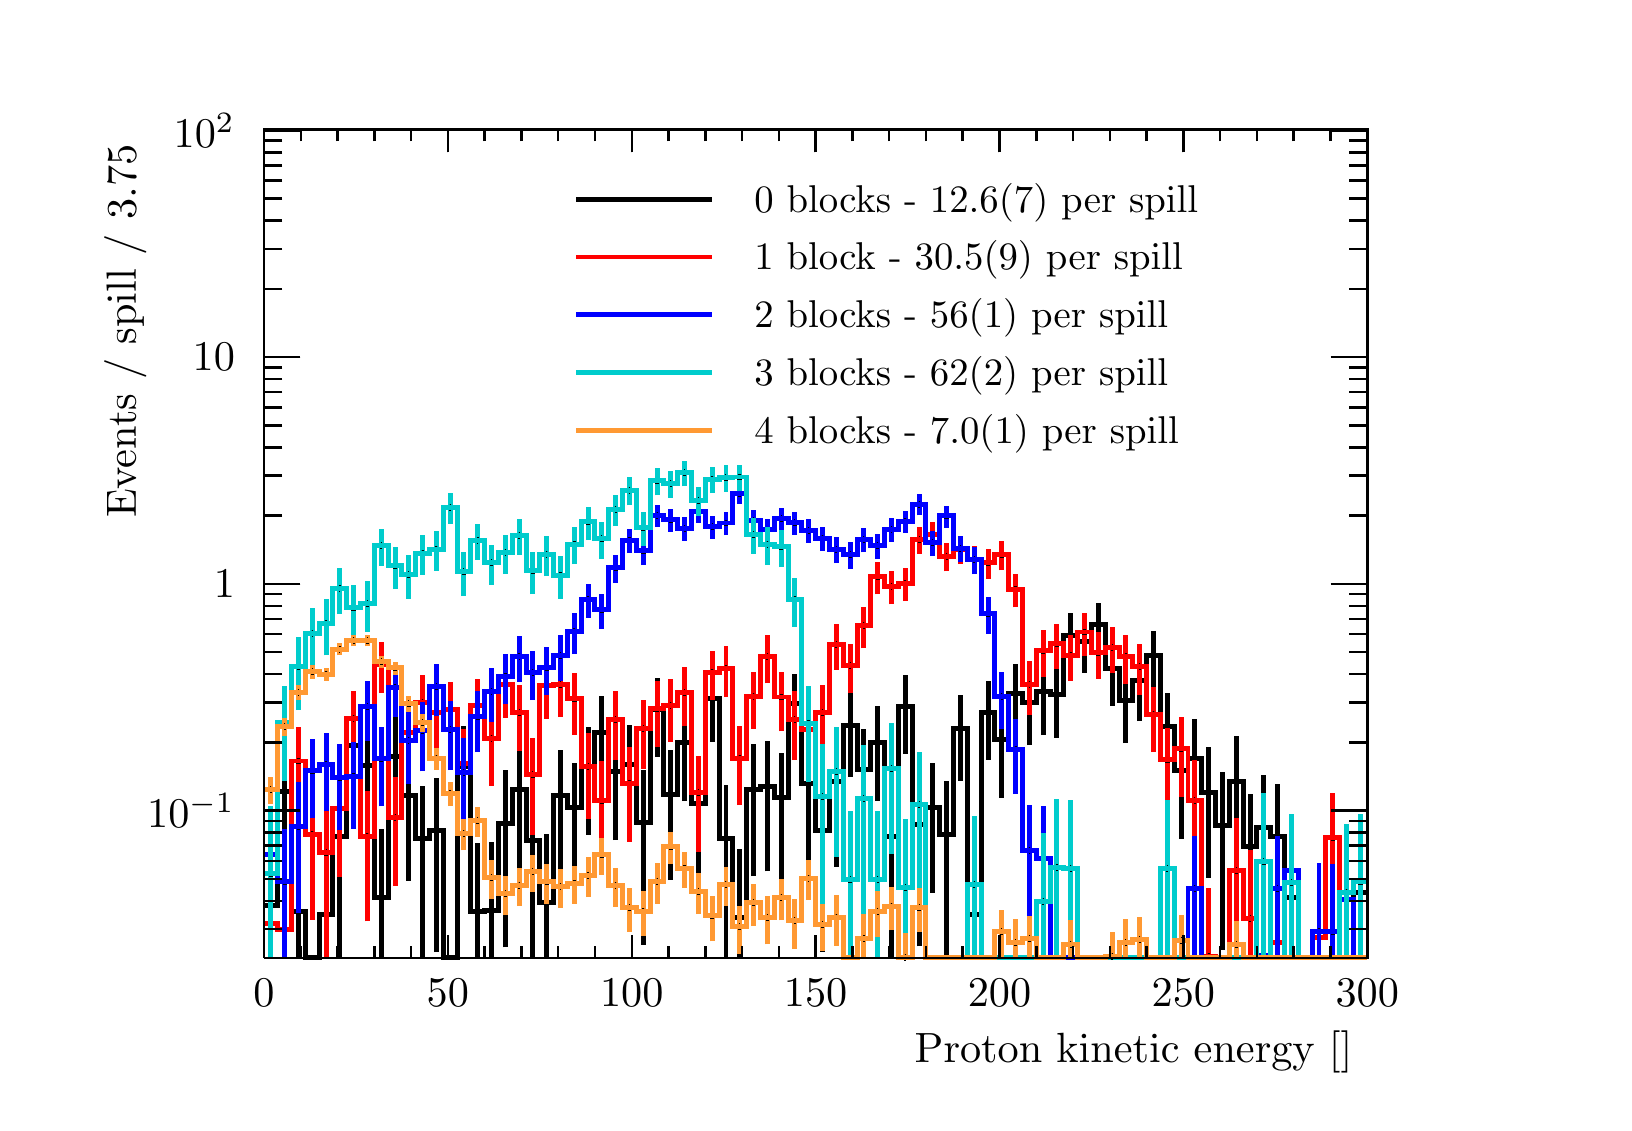
\begin{tikzpicture}
\pgfdeclareplotmark{cross} {
\pgfpathmoveto{\pgfpoint{-0.3\pgfplotmarksize}{\pgfplotmarksize}}
\pgfpathlineto{\pgfpoint{+0.3\pgfplotmarksize}{\pgfplotmarksize}}
\pgfpathlineto{\pgfpoint{+0.3\pgfplotmarksize}{0.3\pgfplotmarksize}}
\pgfpathlineto{\pgfpoint{+1\pgfplotmarksize}{0.3\pgfplotmarksize}}
\pgfpathlineto{\pgfpoint{+1\pgfplotmarksize}{-0.3\pgfplotmarksize}}
\pgfpathlineto{\pgfpoint{+0.3\pgfplotmarksize}{-0.3\pgfplotmarksize}}
\pgfpathlineto{\pgfpoint{+0.3\pgfplotmarksize}{-1.\pgfplotmarksize}}
\pgfpathlineto{\pgfpoint{-0.3\pgfplotmarksize}{-1.\pgfplotmarksize}}
\pgfpathlineto{\pgfpoint{-0.3\pgfplotmarksize}{-0.3\pgfplotmarksize}}
\pgfpathlineto{\pgfpoint{-1.\pgfplotmarksize}{-0.3\pgfplotmarksize}}
\pgfpathlineto{\pgfpoint{-1.\pgfplotmarksize}{0.3\pgfplotmarksize}}
\pgfpathlineto{\pgfpoint{-0.3\pgfplotmarksize}{0.3\pgfplotmarksize}}
\pgfpathclose
\pgfusepathqstroke
}
\pgfdeclareplotmark{cross*} {
\pgfpathmoveto{\pgfpoint{-0.3\pgfplotmarksize}{\pgfplotmarksize}}
\pgfpathlineto{\pgfpoint{+0.3\pgfplotmarksize}{\pgfplotmarksize}}
\pgfpathlineto{\pgfpoint{+0.3\pgfplotmarksize}{0.3\pgfplotmarksize}}
\pgfpathlineto{\pgfpoint{+1\pgfplotmarksize}{0.3\pgfplotmarksize}}
\pgfpathlineto{\pgfpoint{+1\pgfplotmarksize}{-0.3\pgfplotmarksize}}
\pgfpathlineto{\pgfpoint{+0.3\pgfplotmarksize}{-0.3\pgfplotmarksize}}
\pgfpathlineto{\pgfpoint{+0.3\pgfplotmarksize}{-1.\pgfplotmarksize}}
\pgfpathlineto{\pgfpoint{-0.3\pgfplotmarksize}{-1.\pgfplotmarksize}}
\pgfpathlineto{\pgfpoint{-0.3\pgfplotmarksize}{-0.3\pgfplotmarksize}}
\pgfpathlineto{\pgfpoint{-1.\pgfplotmarksize}{-0.3\pgfplotmarksize}}
\pgfpathlineto{\pgfpoint{-1.\pgfplotmarksize}{0.3\pgfplotmarksize}}
\pgfpathlineto{\pgfpoint{-0.3\pgfplotmarksize}{0.3\pgfplotmarksize}}
\pgfpathclose
\pgfusepathqfillstroke
}
\pgfdeclareplotmark{newstar} {
\pgfpathmoveto{\pgfqpoint{0pt}{\pgfplotmarksize}}
\pgfpathlineto{\pgfqpointpolar{44}{0.5\pgfplotmarksize}}
\pgfpathlineto{\pgfqpointpolar{18}{\pgfplotmarksize}}
\pgfpathlineto{\pgfqpointpolar{-20}{0.5\pgfplotmarksize}}
\pgfpathlineto{\pgfqpointpolar{-54}{\pgfplotmarksize}}
\pgfpathlineto{\pgfqpointpolar{-90}{0.5\pgfplotmarksize}}
\pgfpathlineto{\pgfqpointpolar{234}{\pgfplotmarksize}}
\pgfpathlineto{\pgfqpointpolar{198}{0.5\pgfplotmarksize}}
\pgfpathlineto{\pgfqpointpolar{162}{\pgfplotmarksize}}
\pgfpathlineto{\pgfqpointpolar{134}{0.5\pgfplotmarksize}}
\pgfpathclose
\pgfusepathqstroke
}
\pgfdeclareplotmark{newstar*} {
\pgfpathmoveto{\pgfqpoint{0pt}{\pgfplotmarksize}}
\pgfpathlineto{\pgfqpointpolar{44}{0.5\pgfplotmarksize}}
\pgfpathlineto{\pgfqpointpolar{18}{\pgfplotmarksize}}
\pgfpathlineto{\pgfqpointpolar{-20}{0.5\pgfplotmarksize}}
\pgfpathlineto{\pgfqpointpolar{-54}{\pgfplotmarksize}}
\pgfpathlineto{\pgfqpointpolar{-90}{0.5\pgfplotmarksize}}
\pgfpathlineto{\pgfqpointpolar{234}{\pgfplotmarksize}}
\pgfpathlineto{\pgfqpointpolar{198}{0.5\pgfplotmarksize}}
\pgfpathlineto{\pgfqpointpolar{162}{\pgfplotmarksize}}
\pgfpathlineto{\pgfqpointpolar{134}{0.5\pgfplotmarksize}}
\pgfpathclose
\pgfusepathqfillstroke
}
\definecolor{c}{rgb}{1,1,1};
\draw [color=c, fill=c] (0,0) rectangle (20,13.639);
\draw [color=c, fill=c] (2.99427,1.83381) rectangle (17.0057,12.3496);
\definecolor{c}{rgb}{0,0,0};
\draw [c,line width=0.9] (2.99427,1.83381) -- (2.99427,12.3496) -- (17.0057,12.3496) -- (17.0057,1.83381) -- (2.99427,1.83381);
\definecolor{c}{rgb}{1,1,1};
\draw [color=c, fill=c] (2.99427,1.83381) rectangle (17.0057,12.3496);
\definecolor{c}{rgb}{0,0,0};
\draw [c,line width=0.9] (2.99427,1.83381) -- (2.99427,12.3496) -- (17.0057,12.3496) -- (17.0057,1.83381) -- (2.99427,1.83381);
\draw [c,line width=0.9] (2.99427,1.83381) -- (3.16941,1.83381) -- (3.16941,1.83381) -- (3.34456,1.83381) -- (3.34456,1.83381) -- (3.5197,1.83381) -- (3.5197,1.83381) -- (3.69484,1.83381) -- (3.69484,1.83381) -- (3.86999,1.83381) -- (3.86999,1.83381)
 -- (4.04513,1.83381) -- (4.04513,1.83381) -- (4.22027,1.83381) -- (4.22027,1.83381) -- (4.39542,1.83381) -- (4.39542,1.83381) -- (4.57056,1.83381) -- (4.57056,1.83381) -- (4.7457,1.83381) -- (4.7457,1.83381) -- (4.92085,1.83381) -- (4.92085,1.83381)
 -- (5.09599,1.83381) -- (5.09599,1.83381) -- (5.27113,1.83381) -- (5.27113,1.83381) -- (5.44628,1.83381) -- (5.44628,1.83381) -- (5.62142,1.83381) -- (5.62142,1.83381) -- (5.79656,1.83381) -- (5.79656,1.83381) -- (5.9717,1.83381) -- (5.9717,1.83381)
 -- (6.14685,1.83381) -- (6.14685,1.83381) -- (6.32199,1.83381) -- (6.32199,1.83381) -- (6.49713,1.83381) -- (6.49713,1.83381) -- (6.67228,1.83381) -- (6.67228,1.83381) -- (6.84742,1.83381) -- (6.84742,1.83381) -- (7.02256,1.83381) --
 (7.02256,1.83381) -- (7.19771,1.83381) -- (7.19771,1.83381) -- (7.37285,1.83381) -- (7.37285,1.83381) -- (7.54799,1.83381) -- (7.54799,1.83381) -- (7.72314,1.83381) -- (7.72314,1.83381) -- (7.89828,1.83381) -- (7.89828,1.83381) -- (8.07342,1.83381)
 -- (8.07342,1.83381) -- (8.24857,1.83381) -- (8.24857,1.83381) -- (8.42371,1.83381) -- (8.42371,1.83381) -- (8.59885,1.83381) -- (8.59885,1.83381) -- (8.774,1.83381) -- (8.774,1.83381) -- (8.94914,1.83381) -- (8.94914,1.83381) -- (9.12428,1.83381)
 -- (9.12428,1.83381) -- (9.29943,1.83381) -- (9.29943,1.83381) -- (9.47457,1.83381) -- (9.47457,1.83381) -- (9.64971,1.83381) -- (9.64971,1.83381) -- (9.82486,1.83381) -- (9.82486,1.83381) -- (10,1.83381) -- (10,1.83381) -- (10.1751,1.83381) --
 (10.1751,1.83381) -- (10.3503,1.83381) -- (10.3503,1.83381) -- (10.5254,1.83381) -- (10.5254,1.83381) -- (10.7006,1.83381) -- (10.7006,1.83381) -- (10.8757,1.83381) -- (10.8757,1.83381) -- (11.0509,1.83381) -- (11.0509,1.83381) -- (11.226,1.83381)
 -- (11.226,1.83381) -- (11.4011,1.83381) -- (11.4011,1.83381) -- (11.5763,1.83381) -- (11.5763,1.83381) -- (11.7514,1.83381) -- (11.7514,1.83381) -- (11.9266,1.83381) -- (11.9266,1.83381) -- (12.1017,1.83381) -- (12.1017,1.83381) --
 (12.2769,1.83381) -- (12.2769,1.83381) -- (12.452,1.83381) -- (12.452,1.83381) -- (12.6271,1.83381) -- (12.6271,1.83381) -- (12.8023,1.83381) -- (12.8023,1.83381) -- (12.9774,1.83381) -- (12.9774,1.83381) -- (13.1526,1.83381) -- (13.1526,1.83381) --
 (13.3277,1.83381) -- (13.3277,1.83381) -- (13.5029,1.83381) -- (13.5029,1.83381) -- (13.678,1.83381) -- (13.678,1.83381) -- (13.8532,1.83381) -- (13.8532,1.83381) -- (14.0283,1.83381) -- (14.0283,1.83381) -- (14.2034,1.83381) -- (14.2034,1.83381) --
 (14.3786,1.83381) -- (14.3786,1.83381) -- (14.5537,1.83381) -- (14.5537,1.83381) -- (14.7289,1.83381) -- (14.7289,1.83381) -- (14.904,1.83381) -- (14.904,1.83381) -- (15.0792,1.83381) -- (15.0792,1.83381) -- (15.2543,1.83381) -- (15.2543,1.83381) --
 (15.4294,1.83381) -- (15.4294,1.83381) -- (15.6046,1.83381) -- (15.6046,1.83381) -- (15.7797,1.83381) -- (15.7797,1.83381) -- (15.9549,1.83381) -- (15.9549,1.83381) -- (16.13,1.83381) -- (16.13,1.83381) -- (16.3052,1.83381) -- (16.3052,1.83381) --
 (16.4803,1.83381) -- (16.4803,1.83381) -- (16.6554,1.83381) -- (16.6554,1.83381) -- (16.8306,1.83381) -- (16.8306,1.83381) -- (17.0057,1.83381);
\draw [c,line width=0.9] (2.99427,1.83381) -- (17.0057,1.83381);
\draw [c,line width=0.9] (2.99427,2.12046) -- (2.99427,1.83381);
\draw [c,line width=0.9] (3.46132,1.97714) -- (3.46132,1.83381);
\draw [c,line width=0.9] (3.92837,1.97714) -- (3.92837,1.83381);
\draw [c,line width=0.9] (4.39542,1.97714) -- (4.39542,1.83381);
\draw [c,line width=0.9] (4.86246,1.97714) -- (4.86246,1.83381);
\draw [c,line width=0.9] (5.32951,2.12046) -- (5.32951,1.83381);
\draw [c,line width=0.9] (5.79656,1.97714) -- (5.79656,1.83381);
\draw [c,line width=0.9] (6.26361,1.97714) -- (6.26361,1.83381);
\draw [c,line width=0.9] (6.73066,1.97714) -- (6.73066,1.83381);
\draw [c,line width=0.9] (7.19771,1.97714) -- (7.19771,1.83381);
\draw [c,line width=0.9] (7.66476,2.12046) -- (7.66476,1.83381);
\draw [c,line width=0.9] (8.13181,1.97714) -- (8.13181,1.83381);
\draw [c,line width=0.9] (8.59885,1.97714) -- (8.59885,1.83381);
\draw [c,line width=0.9] (9.0659,1.97714) -- (9.0659,1.83381);
\draw [c,line width=0.9] (9.53295,1.97714) -- (9.53295,1.83381);
\draw [c,line width=0.9] (10,2.12046) -- (10,1.83381);
\draw [c,line width=0.9] (10.467,1.97714) -- (10.467,1.83381);
\draw [c,line width=0.9] (10.9341,1.97714) -- (10.9341,1.83381);
\draw [c,line width=0.9] (11.4011,1.97714) -- (11.4011,1.83381);
\draw [c,line width=0.9] (11.8682,1.97714) -- (11.8682,1.83381);
\draw [c,line width=0.9] (12.3352,2.12046) -- (12.3352,1.83381);
\draw [c,line width=0.9] (12.8023,1.97714) -- (12.8023,1.83381);
\draw [c,line width=0.9] (13.2693,1.97714) -- (13.2693,1.83381);
\draw [c,line width=0.9] (13.7364,1.97714) -- (13.7364,1.83381);
\draw [c,line width=0.9] (14.2034,1.97714) -- (14.2034,1.83381);
\draw [c,line width=0.9] (14.6705,2.12046) -- (14.6705,1.83381);
\draw [c,line width=0.9] (15.1375,1.97714) -- (15.1375,1.83381);
\draw [c,line width=0.9] (15.6046,1.97714) -- (15.6046,1.83381);
\draw [c,line width=0.9] (16.0716,1.97714) -- (16.0716,1.83381);
\draw [c,line width=0.9] (16.5387,1.97714) -- (16.5387,1.83381);
\draw [c,line width=0.9] (17.0057,2.12046) -- (17.0057,1.83381);
\draw [anchor=base] (2.99427,1.22006) node[scale=1.52731, color=c, rotate=0]{0};
\draw [anchor=base] (5.32951,1.22006) node[scale=1.52731, color=c, rotate=0]{50};
\draw [anchor=base] (7.66476,1.22006) node[scale=1.52731, color=c, rotate=0]{100};
\draw [anchor=base] (10,1.22006) node[scale=1.52731, color=c, rotate=0]{150};
\draw [anchor=base] (12.3352,1.22006) node[scale=1.52731, color=c, rotate=0]{200};
\draw [anchor=base] (14.6705,1.22006) node[scale=1.52731, color=c, rotate=0]{250};
\draw [anchor=base] (17.0057,1.22006) node[scale=1.52731, color=c, rotate=0]{300};
\draw [anchor= east] (17.0057,0.633582) node[scale=1.52731, color=c, rotate=0]{ Proton kinetic energy [\si{\mega\electronvolt}] };
\draw [c,line width=0.9] (2.99427,12.3496) -- (17.0057,12.3496);
\draw [c,line width=0.9] (2.99427,12.0629) -- (2.99427,12.3496);
\draw [c,line width=0.9] (3.46132,12.2062) -- (3.46132,12.3496);
\draw [c,line width=0.9] (3.92837,12.2062) -- (3.92837,12.3496);
\draw [c,line width=0.9] (4.39542,12.2062) -- (4.39542,12.3496);
\draw [c,line width=0.9] (4.86246,12.2062) -- (4.86246,12.3496);
\draw [c,line width=0.9] (5.32951,12.0629) -- (5.32951,12.3496);
\draw [c,line width=0.9] (5.79656,12.2062) -- (5.79656,12.3496);
\draw [c,line width=0.9] (6.26361,12.2062) -- (6.26361,12.3496);
\draw [c,line width=0.9] (6.73066,12.2062) -- (6.73066,12.3496);
\draw [c,line width=0.9] (7.19771,12.2062) -- (7.19771,12.3496);
\draw [c,line width=0.9] (7.66476,12.0629) -- (7.66476,12.3496);
\draw [c,line width=0.9] (8.13181,12.2062) -- (8.13181,12.3496);
\draw [c,line width=0.9] (8.59885,12.2062) -- (8.59885,12.3496);
\draw [c,line width=0.9] (9.0659,12.2062) -- (9.0659,12.3496);
\draw [c,line width=0.9] (9.53295,12.2062) -- (9.53295,12.3496);
\draw [c,line width=0.9] (10,12.0629) -- (10,12.3496);
\draw [c,line width=0.9] (10.467,12.2062) -- (10.467,12.3496);
\draw [c,line width=0.9] (10.9341,12.2062) -- (10.9341,12.3496);
\draw [c,line width=0.9] (11.4011,12.2062) -- (11.4011,12.3496);
\draw [c,line width=0.9] (11.8682,12.2062) -- (11.8682,12.3496);
\draw [c,line width=0.9] (12.3352,12.0629) -- (12.3352,12.3496);
\draw [c,line width=0.9] (12.8023,12.2062) -- (12.8023,12.3496);
\draw [c,line width=0.9] (13.2693,12.2062) -- (13.2693,12.3496);
\draw [c,line width=0.9] (13.7364,12.2062) -- (13.7364,12.3496);
\draw [c,line width=0.9] (14.2034,12.2062) -- (14.2034,12.3496);
\draw [c,line width=0.9] (14.6705,12.0629) -- (14.6705,12.3496);
\draw [c,line width=0.9] (15.1375,12.2062) -- (15.1375,12.3496);
\draw [c,line width=0.9] (15.6046,12.2062) -- (15.6046,12.3496);
\draw [c,line width=0.9] (16.0716,12.2062) -- (16.0716,12.3496);
\draw [c,line width=0.9] (16.5387,12.2062) -- (16.5387,12.3496);
\draw [c,line width=0.9] (17.0057,12.0629) -- (17.0057,12.3496);
\draw [c,line width=0.9] (2.99427,1.83381) -- (2.99427,12.3496);
\draw [c,line width=0.9] (3.22557,2.1972) -- (2.99427,2.1972);
\draw [c,line width=0.9] (3.22557,2.55698) -- (2.99427,2.55698);
\draw [c,line width=0.9] (3.22557,2.83605) -- (2.99427,2.83605);
\draw [c,line width=0.9] (3.22557,3.06407) -- (2.99427,3.06407);
\draw [c,line width=0.9] (3.22557,3.25685) -- (2.99427,3.25685);
\draw [c,line width=0.9] (3.22557,3.42385) -- (2.99427,3.42385);
\draw [c,line width=0.9] (3.22557,3.57115) -- (2.99427,3.57115);
\draw [c,line width=0.9] (3.45687,3.70292) -- (2.99427,3.70292);
\draw [anchor= east] (2.81427,3.70292) node[scale=1.52731, color=c, rotate=0]{$10^{-1}$};
\draw [c,line width=0.9] (3.22557,4.56979) -- (2.99427,4.56979);
\draw [c,line width=0.9] (3.22557,5.07688) -- (2.99427,5.07688);
\draw [c,line width=0.9] (3.22557,5.43666) -- (2.99427,5.43666);
\draw [c,line width=0.9] (3.22557,5.71573) -- (2.99427,5.71573);
\draw [c,line width=0.9] (3.22557,5.94375) -- (2.99427,5.94375);
\draw [c,line width=0.9] (3.22557,6.13653) -- (2.99427,6.13653);
\draw [c,line width=0.9] (3.22557,6.30353) -- (2.99427,6.30353);
\draw [c,line width=0.9] (3.22557,6.45084) -- (2.99427,6.45084);
\draw [c,line width=0.9] (3.45687,6.5826) -- (2.99427,6.5826);
\draw [anchor= east] (2.81427,6.5826) node[scale=1.52731, color=c, rotate=0]{1};
\draw [c,line width=0.9] (3.22557,7.44947) -- (2.99427,7.44947);
\draw [c,line width=0.9] (3.22557,7.95656) -- (2.99427,7.95656);
\draw [c,line width=0.9] (3.22557,8.31634) -- (2.99427,8.31634);
\draw [c,line width=0.9] (3.22557,8.59541) -- (2.99427,8.59541);
\draw [c,line width=0.9] (3.22557,8.82343) -- (2.99427,8.82343);
\draw [c,line width=0.9] (3.22557,9.01622) -- (2.99427,9.01622);
\draw [c,line width=0.9] (3.22557,9.18321) -- (2.99427,9.18321);
\draw [c,line width=0.9] (3.22557,9.33052) -- (2.99427,9.33052);
\draw [c,line width=0.9] (3.45687,9.46228) -- (2.99427,9.46228);
\draw [anchor= east] (2.81427,9.46228) node[scale=1.52731, color=c, rotate=0]{10};
\draw [c,line width=0.9] (3.22557,10.3292) -- (2.99427,10.3292);
\draw [c,line width=0.9] (3.22557,10.8362) -- (2.99427,10.8362);
\draw [c,line width=0.9] (3.22557,11.196) -- (2.99427,11.196);
\draw [c,line width=0.9] (3.22557,11.4751) -- (2.99427,11.4751);
\draw [c,line width=0.9] (3.22557,11.7031) -- (2.99427,11.7031);
\draw [c,line width=0.9] (3.22557,11.8959) -- (2.99427,11.8959);
\draw [c,line width=0.9] (3.22557,12.0629) -- (2.99427,12.0629);
\draw [c,line width=0.9] (3.22557,12.2102) -- (2.99427,12.2102);
\draw [c,line width=0.9] (3.45687,12.342) -- (2.99427,12.342);
\draw [anchor= east] (2.81427,12.342) node[scale=1.52731, color=c, rotate=0]{$10^{2}$};
\draw [anchor= east] (1.23427,12.3496) node[scale=1.52731, color=c, rotate=90]{ Events / spill / \SI{3.75}{\mega\electronvolt} };
\draw [c,line width=0.9] (17.0057,1.83381) -- (17.0057,12.3496);
\draw [c,line width=0.9] (16.7744,2.1972) -- (17.0057,2.1972);
\draw [c,line width=0.9] (16.7744,2.55698) -- (17.0057,2.55698);
\draw [c,line width=0.9] (16.7744,2.83605) -- (17.0057,2.83605);
\draw [c,line width=0.9] (16.7744,3.06407) -- (17.0057,3.06407);
\draw [c,line width=0.9] (16.7744,3.25685) -- (17.0057,3.25685);
\draw [c,line width=0.9] (16.7744,3.42385) -- (17.0057,3.42385);
\draw [c,line width=0.9] (16.7744,3.57115) -- (17.0057,3.57115);
\draw [c,line width=0.9] (16.5431,3.70292) -- (17.0057,3.70292);
\draw [c,line width=0.9] (16.7744,4.56979) -- (17.0057,4.56979);
\draw [c,line width=0.9] (16.7744,5.07688) -- (17.0057,5.07688);
\draw [c,line width=0.9] (16.7744,5.43666) -- (17.0057,5.43666);
\draw [c,line width=0.9] (16.7744,5.71573) -- (17.0057,5.71573);
\draw [c,line width=0.9] (16.7744,5.94375) -- (17.0057,5.94375);
\draw [c,line width=0.9] (16.7744,6.13653) -- (17.0057,6.13653);
\draw [c,line width=0.9] (16.7744,6.30353) -- (17.0057,6.30353);
\draw [c,line width=0.9] (16.7744,6.45084) -- (17.0057,6.45084);
\draw [c,line width=0.9] (16.5431,6.5826) -- (17.0057,6.5826);
\draw [c,line width=0.9] (16.7744,7.44947) -- (17.0057,7.44947);
\draw [c,line width=0.9] (16.7744,7.95656) -- (17.0057,7.95656);
\draw [c,line width=0.9] (16.7744,8.31634) -- (17.0057,8.31634);
\draw [c,line width=0.9] (16.7744,8.59541) -- (17.0057,8.59541);
\draw [c,line width=0.9] (16.7744,8.82343) -- (17.0057,8.82343);
\draw [c,line width=0.9] (16.7744,9.01622) -- (17.0057,9.01622);
\draw [c,line width=0.9] (16.7744,9.18321) -- (17.0057,9.18321);
\draw [c,line width=0.9] (16.7744,9.33052) -- (17.0057,9.33052);
\draw [c,line width=0.9] (16.5431,9.46228) -- (17.0057,9.46228);
\draw [c,line width=0.9] (16.7744,10.3292) -- (17.0057,10.3292);
\draw [c,line width=0.9] (16.7744,10.8362) -- (17.0057,10.8362);
\draw [c,line width=0.9] (16.7744,11.196) -- (17.0057,11.196);
\draw [c,line width=0.9] (16.7744,11.4751) -- (17.0057,11.4751);
\draw [c,line width=0.9] (16.7744,11.7031) -- (17.0057,11.7031);
\draw [c,line width=0.9] (16.7744,11.8959) -- (17.0057,11.8959);
\draw [c,line width=0.9] (16.7744,12.0629) -- (17.0057,12.0629);
\draw [c,line width=0.9] (16.7744,12.2102) -- (17.0057,12.2102);
\draw [c,line width=0.9] (16.5431,12.342) -- (17.0057,12.342);
\draw [c,line width=1.8] (3.08184,1.83381) -- (3.08184,2.49495);
\draw [c,line width=1.8] (3.08184,2.49495) -- (3.08184,3.36182);
\foreach \P in {(3.08184,2.49495)}{\draw[mark options={color=c,fill=c},mark size=2.402402pt, line width=0.000000pt, mark=*,mark size=1pt] plot coordinates {\P};}
\draw [c,line width=1.8] (3.25698,2.86262) -- (3.25698,3.94086);
\draw [c,line width=1.8] (3.25698,3.94086) -- (3.25698,4.51115);
\foreach \P in {(3.25698,3.94086)}{\draw[mark options={color=c,fill=c},mark size=2.402402pt, line width=0.000000pt, mark=*,mark size=1pt] plot coordinates {\P};}
\draw [c,line width=1.8] (3.43213,1.83381) -- (3.43213,2.41884);
\draw [c,line width=1.8] (3.43213,2.41884) -- (3.43213,3.28571);
\foreach \P in {(3.43213,2.41884)}{\draw[mark options={color=c,fill=c},mark size=2.402402pt, line width=0.000000pt, mark=*,mark size=1pt] plot coordinates {\P};}
\draw [c,line width=1.8] (3.78241,1.83381) -- (3.78241,2.37847);
\draw [c,line width=1.8] (3.78241,2.37847) -- (3.78241,3.24535);
\foreach \P in {(3.78241,2.37847)}{\draw[mark options={color=c,fill=c},mark size=2.402402pt, line width=0.000000pt, mark=*,mark size=1pt] plot coordinates {\P};}
\draw [c,line width=1.8] (3.95756,1.83619) -- (3.95756,3.37699);
\draw [c,line width=1.8] (3.95756,3.37699) -- (3.95756,4.04669);
\foreach \P in {(3.95756,3.37699)}{\draw[mark options={color=c,fill=c},mark size=2.402402pt, line width=0.000000pt, mark=*,mark size=1pt] plot coordinates {\P};}
\draw [c,line width=1.8] (4.1327,3.78699) -- (4.1327,4.52859);
\draw [c,line width=1.8] (4.1327,4.52859) -- (4.1327,4.99097);
\foreach \P in {(4.1327,4.52859)}{\draw[mark options={color=c,fill=c},mark size=2.402402pt, line width=0.000000pt, mark=*,mark size=1pt] plot coordinates {\P};}
\draw [c,line width=1.8] (4.30784,3.40697) -- (4.30784,4.27776);
\draw [c,line width=1.8] (4.30784,4.27776) -- (4.30784,4.78616);
\foreach \P in {(4.30784,4.27776)}{\draw[mark options={color=c,fill=c},mark size=2.402402pt, line width=0.000000pt, mark=*,mark size=1pt] plot coordinates {\P};}
\draw [c,line width=1.8] (4.48299,1.83381) -- (4.48299,2.59947);
\draw [c,line width=1.8] (4.48299,2.59947) -- (4.48299,3.46634);
\foreach \P in {(4.48299,2.59947)}{\draw[mark options={color=c,fill=c},mark size=2.402402pt, line width=0.000000pt, mark=*,mark size=1pt] plot coordinates {\P};}
\draw [c,line width=1.8] (4.65813,3.51155) -- (4.65813,4.38886);
\draw [c,line width=1.8] (4.65813,4.38886) -- (4.65813,4.89941);
\foreach \P in {(4.65813,4.38886)}{\draw[mark options={color=c,fill=c},mark size=2.402402pt, line width=0.000000pt, mark=*,mark size=1pt] plot coordinates {\P};}
\draw [c,line width=1.8] (4.83327,2.81138) -- (4.83327,3.88956);
\draw [c,line width=1.8] (4.83327,3.88956) -- (4.83327,4.45983);
\foreach \P in {(4.83327,3.88956)}{\draw[mark options={color=c,fill=c},mark size=2.402402pt, line width=0.000000pt, mark=*,mark size=1pt] plot coordinates {\P};}
\draw [c,line width=1.8] (5.00842,1.83381) -- (5.00842,3.34364);
\draw [c,line width=1.8] (5.00842,3.34364) -- (5.00842,4.01834);
\foreach \P in {(5.00842,3.34364)}{\draw[mark options={color=c,fill=c},mark size=2.402402pt, line width=0.000000pt, mark=*,mark size=1pt] plot coordinates {\P};}
\draw [c,line width=1.8] (5.18356,1.90655) -- (5.18356,3.44579);
\draw [c,line width=1.8] (5.18356,3.44579) -- (5.18356,4.11523);
\foreach \P in {(5.18356,3.44579)}{\draw[mark options={color=c,fill=c},mark size=2.402402pt, line width=0.000000pt, mark=*,mark size=1pt] plot coordinates {\P};}
\draw [c,line width=1.8] (5.53385,3.38859) -- (5.53385,4.26171);
\draw [c,line width=1.8] (5.53385,4.26171) -- (5.53385,4.77088);
\foreach \P in {(5.53385,4.26171)}{\draw[mark options={color=c,fill=c},mark size=2.402402pt, line width=0.000000pt, mark=*,mark size=1pt] plot coordinates {\P};}
\draw [c,line width=1.8] (5.70899,1.83381) -- (5.70899,2.41884);
\draw [c,line width=1.8] (5.70899,2.41884) -- (5.70899,3.28571);
\foreach \P in {(5.70899,2.41884)}{\draw[mark options={color=c,fill=c},mark size=2.402402pt, line width=0.000000pt, mark=*,mark size=1pt] plot coordinates {\P};}
\draw [c,line width=1.8] (5.88413,1.83381) -- (5.88413,2.43536);
\draw [c,line width=1.8] (5.88413,2.43536) -- (5.88413,3.30223);
\foreach \P in {(5.88413,2.43536)}{\draw[mark options={color=c,fill=c},mark size=2.402402pt, line width=0.000000pt, mark=*,mark size=1pt] plot coordinates {\P};}
\draw [c,line width=1.8] (6.05928,1.96707) -- (6.05928,3.54418);
\draw [c,line width=1.8] (6.05928,3.54418) -- (6.05928,4.21998);
\foreach \P in {(6.05928,3.54418)}{\draw[mark options={color=c,fill=c},mark size=2.402402pt, line width=0.000000pt, mark=*,mark size=1pt] plot coordinates {\P};}
\draw [c,line width=1.8] (6.23442,2.87278) -- (6.23442,3.97116);
\draw [c,line width=1.8] (6.23442,3.97116) -- (6.23442,4.54678);
\foreach \P in {(6.23442,3.97116)}{\draw[mark options={color=c,fill=c},mark size=2.402402pt, line width=0.000000pt, mark=*,mark size=1pt] plot coordinates {\P};}
\draw [c,line width=1.8] (6.40956,1.83381) -- (6.40956,3.32794);
\draw [c,line width=1.8] (6.40956,3.32794) -- (6.40956,3.99688);
\foreach \P in {(6.40956,3.32794)}{\draw[mark options={color=c,fill=c},mark size=2.402402pt, line width=0.000000pt, mark=*,mark size=1pt] plot coordinates {\P};}
\draw [c,line width=1.8] (6.58471,1.83381) -- (6.58471,2.53932);
\draw [c,line width=1.8] (6.58471,2.53932) -- (6.58471,3.4062);
\foreach \P in {(6.58471,2.53932)}{\draw[mark options={color=c,fill=c},mark size=2.402402pt, line width=0.000000pt, mark=*,mark size=1pt] plot coordinates {\P};}
\draw [c,line width=1.8] (6.75985,2.81802) -- (6.75985,3.89755);
\draw [c,line width=1.8] (6.75985,3.89755) -- (6.75985,4.46818);
\foreach \P in {(6.75985,3.89755)}{\draw[mark options={color=c,fill=c},mark size=2.402402pt, line width=0.000000pt, mark=*,mark size=1pt] plot coordinates {\P};}
\draw [c,line width=1.8] (6.93499,2.66114) -- (6.93499,3.73874);
\draw [c,line width=1.8] (6.93499,3.73874) -- (6.93499,4.30885);
\foreach \P in {(6.93499,3.73874)}{\draw[mark options={color=c,fill=c},mark size=2.402402pt, line width=0.000000pt, mark=*,mark size=1pt] plot coordinates {\P};}
\draw [c,line width=1.8] (7.11014,3.39419) -- (7.11014,4.26249);
\draw [c,line width=1.8] (7.11014,4.26249) -- (7.11014,4.77005);
\foreach \P in {(7.11014,4.26249)}{\draw[mark options={color=c,fill=c},mark size=2.402402pt, line width=0.000000pt, mark=*,mark size=1pt] plot coordinates {\P};}
\draw [c,line width=1.8] (7.28528,3.94216) -- (7.28528,4.69077);
\draw [c,line width=1.8] (7.28528,4.69077) -- (7.28528,5.15581);
\foreach \P in {(7.28528,4.69077)}{\draw[mark options={color=c,fill=c},mark size=2.402402pt, line width=0.000000pt, mark=*,mark size=1pt] plot coordinates {\P};}
\draw [c,line width=1.8] (7.46042,3.32697) -- (7.46042,4.19778);
\draw [c,line width=1.8] (7.46042,4.19778) -- (7.46042,4.70618);
\foreach \P in {(7.46042,4.19778)}{\draw[mark options={color=c,fill=c},mark size=2.402402pt, line width=0.000000pt, mark=*,mark size=1pt] plot coordinates {\P};}
\draw [c,line width=1.8] (7.63557,3.41001) -- (7.63557,4.28309);
\draw [c,line width=1.8] (7.63557,4.28309) -- (7.63557,4.79223);
\foreach \P in {(7.63557,4.28309)}{\draw[mark options={color=c,fill=c},mark size=2.402402pt, line width=0.000000pt, mark=*,mark size=1pt] plot coordinates {\P};}
\draw [c,line width=1.8] (7.81071,1.99602) -- (7.81071,3.54814);
\draw [c,line width=1.8] (7.81071,3.54814) -- (7.81071,4.21977);
\foreach \P in {(7.81071,3.54814)}{\draw[mark options={color=c,fill=c},mark size=2.402402pt, line width=0.000000pt, mark=*,mark size=1pt] plot coordinates {\P};}
\draw [c,line width=1.8] (7.98585,4.3864) -- (7.98585,4.98521);
\draw [c,line width=1.8] (7.98585,4.98521) -- (7.98585,5.38845);
\foreach \P in {(7.98585,4.98521)}{\draw[mark options={color=c,fill=c},mark size=2.402402pt, line width=0.000000pt, mark=*,mark size=1pt] plot coordinates {\P};}
\draw [c,line width=1.8] (8.161,2.81948) -- (8.161,3.90276);
\draw [c,line width=1.8] (8.161,3.90276) -- (8.161,4.47439);
\foreach \P in {(8.161,3.90276)}{\draw[mark options={color=c,fill=c},mark size=2.402402pt, line width=0.000000pt, mark=*,mark size=1pt] plot coordinates {\P};}
\draw [c,line width=1.8] (8.33614,3.82405) -- (8.33614,4.56876);
\draw [c,line width=1.8] (8.33614,4.56876) -- (8.33614,5.03232);
\foreach \P in {(8.33614,4.56876)}{\draw[mark options={color=c,fill=c},mark size=2.402402pt, line width=0.000000pt, mark=*,mark size=1pt] plot coordinates {\P};}
\draw [c,line width=1.8] (8.51128,2.71359) -- (8.51128,3.79853);
\draw [c,line width=1.8] (8.51128,3.79853) -- (8.51128,4.3706);
\foreach \P in {(8.51128,3.79853)}{\draw[mark options={color=c,fill=c},mark size=2.402402pt, line width=0.000000pt, mark=*,mark size=1pt] plot coordinates {\P};}
\draw [c,line width=1.8] (8.68643,4.57708) -- (8.68643,5.12508);
\draw [c,line width=1.8] (8.68643,5.12508) -- (8.68643,5.50482);
\foreach \P in {(8.68643,5.12508)}{\draw[mark options={color=c,fill=c},mark size=2.402402pt, line width=0.000000pt, mark=*,mark size=1pt] plot coordinates {\P};}
\draw [c,line width=1.8] (8.86157,1.83381) -- (8.86157,3.35002);
\draw [c,line width=1.8] (8.86157,3.35002) -- (8.86157,4.02175);
\foreach \P in {(8.86157,3.35002)}{\draw[mark options={color=c,fill=c},mark size=2.402402pt, line width=0.000000pt, mark=*,mark size=1pt] plot coordinates {\P};}
\draw [c,line width=1.8] (9.03671,1.83381) -- (9.03671,2.34323);
\draw [c,line width=1.8] (9.03671,2.34323) -- (9.03671,3.2101);
\foreach \P in {(9.03671,2.34323)}{\draw[mark options={color=c,fill=c},mark size=2.402402pt, line width=0.000000pt, mark=*,mark size=1pt] plot coordinates {\P};}
\draw [c,line width=1.8] (9.21185,2.872) -- (9.21185,3.96747);
\draw [c,line width=1.8] (9.21185,3.96747) -- (9.21185,4.54233);
\foreach \P in {(9.21185,3.96747)}{\draw[mark options={color=c,fill=c},mark size=2.402402pt, line width=0.000000pt, mark=*,mark size=1pt] plot coordinates {\P};}
\draw [c,line width=1.8] (9.387,2.93255) -- (9.387,4.0147);
\draw [c,line width=1.8] (9.387,4.0147) -- (9.387,4.58604);
\foreach \P in {(9.387,4.0147)}{\draw[mark options={color=c,fill=c},mark size=2.402402pt, line width=0.000000pt, mark=*,mark size=1pt] plot coordinates {\P};}
\draw [c,line width=1.8] (9.56214,2.79071) -- (9.56214,3.86849);
\draw [c,line width=1.8] (9.56214,3.86849) -- (9.56214,4.43865);
\foreach \P in {(9.56214,3.86849)}{\draw[mark options={color=c,fill=c},mark size=2.402402pt, line width=0.000000pt, mark=*,mark size=1pt] plot coordinates {\P};}
\draw [c,line width=1.8] (9.73728,4.51511) -- (9.73728,5.06213);
\draw [c,line width=1.8] (9.73728,5.06213) -- (9.73728,5.44141);
\foreach \P in {(9.73728,5.06213)}{\draw[mark options={color=c,fill=c},mark size=2.402402pt, line width=0.000000pt, mark=*,mark size=1pt] plot coordinates {\P};}
\draw [c,line width=1.8] (9.91243,2.96131) -- (9.91243,4.04165);
\draw [c,line width=1.8] (9.91243,4.04165) -- (9.91243,4.6125);
\foreach \P in {(9.91243,4.04165)}{\draw[mark options={color=c,fill=c},mark size=2.402402pt, line width=0.000000pt, mark=*,mark size=1pt] plot coordinates {\P};}
\draw [c,line width=1.8] (10.0876,1.90944) -- (10.0876,3.44541);
\draw [c,line width=1.8] (10.0876,3.44541) -- (10.0876,4.11429);
\foreach \P in {(10.0876,3.44541)}{\draw[mark options={color=c,fill=c},mark size=2.402402pt, line width=0.000000pt, mark=*,mark size=1pt] plot coordinates {\P};}
\draw [c,line width=1.8] (10.2627,2.98757) -- (10.2627,4.06736);
\draw [c,line width=1.8] (10.2627,4.06736) -- (10.2627,4.63806);
\foreach \P in {(10.2627,4.06736)}{\draw[mark options={color=c,fill=c},mark size=2.402402pt, line width=0.000000pt, mark=*,mark size=1pt] plot coordinates {\P};}
\draw [c,line width=1.8] (10.4379,4.13142) -- (10.4379,4.78978);
\draw [c,line width=1.8] (10.4379,4.78978) -- (10.4379,5.21885);
\foreach \P in {(10.4379,4.78978)}{\draw[mark options={color=c,fill=c},mark size=2.402402pt, line width=0.000000pt, mark=*,mark size=1pt] plot coordinates {\P};}
\draw [c,line width=1.8] (10.613,3.35897) -- (10.613,4.22719);
\draw [c,line width=1.8] (10.613,4.22719) -- (10.613,4.73473);
\foreach \P in {(10.613,4.22719)}{\draw[mark options={color=c,fill=c},mark size=2.402402pt, line width=0.000000pt, mark=*,mark size=1pt] plot coordinates {\P};}
\draw [c,line width=1.8] (10.7881,3.82436) -- (10.7881,4.56688);
\draw [c,line width=1.8] (10.7881,4.56688) -- (10.7881,5.02961);
\foreach \P in {(10.7881,4.56688)}{\draw[mark options={color=c,fill=c},mark size=2.402402pt, line width=0.000000pt, mark=*,mark size=1pt] plot coordinates {\P};}
\draw [c,line width=1.8] (10.9633,1.83381) -- (10.9633,3.37423);
\draw [c,line width=1.8] (10.9633,3.37423) -- (10.9633,4.04428);
\foreach \P in {(10.9633,3.37423)}{\draw[mark options={color=c,fill=c},mark size=2.402402pt, line width=0.000000pt, mark=*,mark size=1pt] plot coordinates {\P};}
\draw [c,line width=1.8] (11.1384,4.42589) -- (11.1384,5.02374);
\draw [c,line width=1.8] (11.1384,5.02374) -- (11.1384,5.42655);
\foreach \P in {(11.1384,5.02374)}{\draw[mark options={color=c,fill=c},mark size=2.402402pt, line width=0.000000pt, mark=*,mark size=1pt] plot coordinates {\P};}
\draw [c,line width=1.8] (11.3136,1.97701) -- (11.3136,3.52409);
\draw [c,line width=1.8] (11.3136,3.52409) -- (11.3136,4.19486);
\foreach \P in {(11.3136,3.52409)}{\draw[mark options={color=c,fill=c},mark size=2.402402pt, line width=0.000000pt, mark=*,mark size=1pt] plot coordinates {\P};}
\draw [c,line width=1.8] (11.4887,2.66098) -- (11.4887,3.73823);
\draw [c,line width=1.8] (11.4887,3.73823) -- (11.4887,4.30825);
\foreach \P in {(11.4887,3.73823)}{\draw[mark options={color=c,fill=c},mark size=2.402402pt, line width=0.000000pt, mark=*,mark size=1pt] plot coordinates {\P};}
\draw [c,line width=1.8] (11.6639,1.83381) -- (11.6639,3.39806);
\draw [c,line width=1.8] (11.6639,3.39806) -- (11.6639,4.07248);
\foreach \P in {(11.6639,3.39806)}{\draw[mark options={color=c,fill=c},mark size=2.402402pt, line width=0.000000pt, mark=*,mark size=1pt] plot coordinates {\P};}
\draw [c,line width=1.8] (11.839,4.08427) -- (11.839,4.74138);
\draw [c,line width=1.8] (11.839,4.74138) -- (11.839,5.16993);
\foreach \P in {(11.839,4.74138)}{\draw[mark options={color=c,fill=c},mark size=2.402402pt, line width=0.000000pt, mark=*,mark size=1pt] plot coordinates {\P};}
\draw [c,line width=1.8] (12.0141,1.83381) -- (12.0141,2.38644);
\draw [c,line width=1.8] (12.0141,2.38644) -- (12.0141,3.25331);
\foreach \P in {(12.0141,2.38644)}{\draw[mark options={color=c,fill=c},mark size=2.402402pt, line width=0.000000pt, mark=*,mark size=1pt] plot coordinates {\P};}
\draw [c,line width=1.8] (12.1893,4.34779) -- (12.1893,4.94584);
\draw [c,line width=1.8] (12.1893,4.94584) -- (12.1893,5.34873);
\foreach \P in {(12.1893,4.94584)}{\draw[mark options={color=c,fill=c},mark size=2.402402pt, line width=0.000000pt, mark=*,mark size=1pt] plot coordinates {\P};}
\draw [c,line width=1.8] (12.3644,3.86419) -- (12.3644,4.60612);
\draw [c,line width=1.8] (12.3644,4.60612) -- (12.3644,5.06862);
\foreach \P in {(12.3644,4.60612)}{\draw[mark options={color=c,fill=c},mark size=2.402402pt, line width=0.000000pt, mark=*,mark size=1pt] plot coordinates {\P};}
\draw [c,line width=1.8] (12.5396,4.63861) -- (12.5396,5.18953);
\draw [c,line width=1.8] (12.5396,5.18953) -- (12.5396,5.57067);
\foreach \P in {(12.5396,5.18953)}{\draw[mark options={color=c,fill=c},mark size=2.402402pt, line width=0.000000pt, mark=*,mark size=1pt] plot coordinates {\P};}
\draw [c,line width=1.8] (12.7147,4.53483) -- (12.7147,5.08152);
\draw [c,line width=1.8] (12.7147,5.08152) -- (12.7147,5.46064);
\foreach \P in {(12.7147,5.08152)}{\draw[mark options={color=c,fill=c},mark size=2.402402pt, line width=0.000000pt, mark=*,mark size=1pt] plot coordinates {\P};}
\draw [c,line width=1.8] (12.8899,4.66051) -- (12.8899,5.21061);
\draw [c,line width=1.8] (12.8899,5.21061) -- (12.8899,5.59136);
\foreach \P in {(12.8899,5.21061)}{\draw[mark options={color=c,fill=c},mark size=2.402402pt, line width=0.000000pt, mark=*,mark size=1pt] plot coordinates {\P};}
\draw [c,line width=1.8] (13.065,4.62868) -- (13.065,5.18022);
\draw [c,line width=1.8] (13.065,5.18022) -- (13.065,5.56166);
\foreach \P in {(13.065,5.18022)}{\draw[mark options={color=c,fill=c},mark size=2.402402pt, line width=0.000000pt, mark=*,mark size=1pt] plot coordinates {\P};}
\draw [c,line width=1.8] (13.2402,5.54448) -- (13.2402,5.92074);
\draw [c,line width=1.8] (13.2402,5.92074) -- (13.2402,6.2096);
\foreach \P in {(13.2402,5.92074)}{\draw[mark options={color=c,fill=c},mark size=2.402402pt, line width=0.000000pt, mark=*,mark size=1pt] plot coordinates {\P};}
\draw [c,line width=1.8] (13.4153,5.45423) -- (13.4153,5.84615);
\draw [c,line width=1.8] (13.4153,5.84615) -- (13.4153,6.14411);
\foreach \P in {(13.4153,5.84615)}{\draw[mark options={color=c,fill=c},mark size=2.402402pt, line width=0.000000pt, mark=*,mark size=1pt] plot coordinates {\P};}
\draw [c,line width=1.8] (13.5904,5.69936) -- (13.5904,6.06117);
\draw [c,line width=1.8] (13.5904,6.06117) -- (13.5904,6.34146);
\foreach \P in {(13.5904,6.06117)}{\draw[mark options={color=c,fill=c},mark size=2.402402pt, line width=0.000000pt, mark=*,mark size=1pt] plot coordinates {\P};}
\draw [c,line width=1.8] (13.7656,5.03392) -- (13.7656,5.51116);
\draw [c,line width=1.8] (13.7656,5.51116) -- (13.7656,5.85576);
\foreach \P in {(13.7656,5.51116)}{\draw[mark options={color=c,fill=c},mark size=2.402402pt, line width=0.000000pt, mark=*,mark size=1pt] plot coordinates {\P};}
\draw [c,line width=1.8] (13.9407,4.55917) -- (13.9407,5.1063);
\draw [c,line width=1.8] (13.9407,5.1063) -- (13.9407,5.48564);
\foreach \P in {(13.9407,5.1063)}{\draw[mark options={color=c,fill=c},mark size=2.402402pt, line width=0.000000pt, mark=*,mark size=1pt] plot coordinates {\P};}
\draw [c,line width=1.8] (14.1159,4.83982) -- (14.1159,5.35166);
\draw [c,line width=1.8] (14.1159,5.35166) -- (14.1159,5.71382);
\foreach \P in {(14.1159,5.35166)}{\draw[mark options={color=c,fill=c},mark size=2.402402pt, line width=0.000000pt, mark=*,mark size=1pt] plot coordinates {\P};}
\draw [c,line width=1.8] (14.291,5.24018) -- (14.291,5.66843);
\draw [c,line width=1.8] (14.291,5.66843) -- (14.291,5.98684);
\foreach \P in {(14.291,5.66843)}{\draw[mark options={color=c,fill=c},mark size=2.402402pt, line width=0.000000pt, mark=*,mark size=1pt] plot coordinates {\P};}
\draw [c,line width=1.8] (14.4662,4.10354) -- (14.4662,4.76567);
\draw [c,line width=1.8] (14.4662,4.76567) -- (14.4662,5.19632);
\foreach \P in {(14.4662,4.76567)}{\draw[mark options={color=c,fill=c},mark size=2.402402pt, line width=0.000000pt, mark=*,mark size=1pt] plot coordinates {\P};}
\draw [c,line width=1.8] (14.6413,3.34468) -- (14.6413,4.21292);
\draw [c,line width=1.8] (14.6413,4.21292) -- (14.6413,4.72047);
\foreach \P in {(14.6413,4.21292)}{\draw[mark options={color=c,fill=c},mark size=2.402402pt, line width=0.000000pt, mark=*,mark size=1pt] plot coordinates {\P};}
\draw [c,line width=1.8] (14.8164,3.49683) -- (14.8164,4.36421);
\draw [c,line width=1.8] (14.8164,4.36421) -- (14.8164,4.87146);
\foreach \P in {(14.8164,4.36421)}{\draw[mark options={color=c,fill=c},mark size=2.402402pt, line width=0.000000pt, mark=*,mark size=1pt] plot coordinates {\P};}
\draw [c,line width=1.8] (14.9916,2.84977) -- (14.9916,3.93321);
\draw [c,line width=1.8] (14.9916,3.93321) -- (14.9916,4.50489);
\foreach \P in {(14.9916,3.93321)}{\draw[mark options={color=c,fill=c},mark size=2.402402pt, line width=0.000000pt, mark=*,mark size=1pt] plot coordinates {\P};}
\draw [c,line width=1.8] (15.1667,1.93764) -- (15.1667,3.51674);
\draw [c,line width=1.8] (15.1667,3.51674) -- (15.1667,4.19287);
\foreach \P in {(15.1667,3.51674)}{\draw[mark options={color=c,fill=c},mark size=2.402402pt, line width=0.000000pt, mark=*,mark size=1pt] plot coordinates {\P};}
\draw [c,line width=1.8] (15.3419,2.993) -- (15.3419,4.07847);
\draw [c,line width=1.8] (15.3419,4.07847) -- (15.3419,4.65069);
\foreach \P in {(15.3419,4.07847)}{\draw[mark options={color=c,fill=c},mark size=2.402402pt, line width=0.000000pt, mark=*,mark size=1pt] plot coordinates {\P};}
\draw [c,line width=1.8] (15.517,1.83381) -- (15.517,3.24218);
\draw [c,line width=1.8] (15.517,3.24218) -- (15.517,3.91119);
\foreach \P in {(15.517,3.24218)}{\draw[mark options={color=c,fill=c},mark size=2.402402pt, line width=0.000000pt, mark=*,mark size=1pt] plot coordinates {\P};}
\draw [c,line width=1.8] (15.6922,1.94706) -- (15.6922,3.48438);
\draw [c,line width=1.8] (15.6922,3.48438) -- (15.6922,4.15349);
\foreach \P in {(15.6922,3.48438)}{\draw[mark options={color=c,fill=c},mark size=2.402402pt, line width=0.000000pt, mark=*,mark size=1pt] plot coordinates {\P};}
\draw [c,line width=1.8] (15.8673,1.83381) -- (15.8673,3.3692);
\draw [c,line width=1.8] (15.8673,3.3692) -- (15.8673,4.03956);
\foreach \P in {(15.8673,3.3692)}{\draw[mark options={color=c,fill=c},mark size=2.402402pt, line width=0.000000pt, mark=*,mark size=1pt] plot coordinates {\P};}
\draw [c,line width=1.8] (16.0424,1.83381) -- (16.0424,2.59474);
\draw [c,line width=1.8] (16.0424,2.59474) -- (16.0424,3.46161);
\foreach \P in {(16.0424,2.59474)}{\draw[mark options={color=c,fill=c},mark size=2.402402pt, line width=0.000000pt, mark=*,mark size=1pt] plot coordinates {\P};}
\draw [c,line width=1.8] (16.9182,1.83381) -- (16.9182,2.66266);
\draw [c,line width=1.8] (16.9182,2.66266) -- (16.9182,3.52953);
\foreach \P in {(16.9182,2.66266)}{\draw[mark options={color=c,fill=c},mark size=2.402402pt, line width=0.000000pt, mark=*,mark size=1pt] plot coordinates {\P};}
\draw [c,line width=1.8] (2.99427,2.49495) -- (3.16941,2.49495) -- (3.16941,3.94086) -- (3.34456,3.94086) -- (3.34456,2.41884) -- (3.5197,2.41884) -- (3.5197,1.83381) -- (3.69484,1.83381) -- (3.69484,2.37847) -- (3.86999,2.37847) -- (3.86999,3.37699)
 -- (4.04513,3.37699) -- (4.04513,4.52859) -- (4.22027,4.52859) -- (4.22027,4.27776) -- (4.39542,4.27776) -- (4.39542,2.59947) -- (4.57056,2.59947) -- (4.57056,4.38886) -- (4.7457,4.38886) -- (4.7457,3.88956) -- (4.92085,3.88956) -- (4.92085,3.34364)
 -- (5.09599,3.34364) -- (5.09599,3.44579) -- (5.27113,3.44579) -- (5.27113,1.83381) -- (5.44628,1.83381) -- (5.44628,4.26171) -- (5.62142,4.26171) -- (5.62142,2.41884) -- (5.79656,2.41884) -- (5.79656,2.43536) -- (5.9717,2.43536) -- (5.9717,3.54418)
 -- (6.14685,3.54418) -- (6.14685,3.97116) -- (6.32199,3.97116) -- (6.32199,3.32794) -- (6.49713,3.32794) -- (6.49713,2.53932) -- (6.67228,2.53932) -- (6.67228,3.89755) -- (6.84742,3.89755) -- (6.84742,3.73874) -- (7.02256,3.73874) --
 (7.02256,4.26249) -- (7.19771,4.26249) -- (7.19771,4.69077) -- (7.37285,4.69077) -- (7.37285,4.19778) -- (7.54799,4.19778) -- (7.54799,4.28309) -- (7.72314,4.28309) -- (7.72314,3.54814) -- (7.89828,3.54814) -- (7.89828,4.98521) -- (8.07342,4.98521)
 -- (8.07342,3.90276) -- (8.24857,3.90276) -- (8.24857,4.56876) -- (8.42371,4.56876) -- (8.42371,3.79853) -- (8.59885,3.79853) -- (8.59885,5.12508) -- (8.774,5.12508) -- (8.774,3.35002) -- (8.94914,3.35002) -- (8.94914,2.34323) -- (9.12428,2.34323)
 -- (9.12428,3.96747) -- (9.29943,3.96747) -- (9.29943,4.0147) -- (9.47457,4.0147) -- (9.47457,3.86849) -- (9.64971,3.86849) -- (9.64971,5.06213) -- (9.82486,5.06213) -- (9.82486,4.04165) -- (10,4.04165) -- (10,3.44541) -- (10.1751,3.44541) --
 (10.1751,4.06736) -- (10.3503,4.06736) -- (10.3503,4.78978) -- (10.5254,4.78978) -- (10.5254,4.22719) -- (10.7006,4.22719) -- (10.7006,4.56688) -- (10.8757,4.56688) -- (10.8757,3.37423) -- (11.0509,3.37423) -- (11.0509,5.02374) -- (11.226,5.02374)
 -- (11.226,3.52409) -- (11.4011,3.52409) -- (11.4011,3.73823) -- (11.5763,3.73823) -- (11.5763,3.39806) -- (11.7514,3.39806) -- (11.7514,4.74138) -- (11.9266,4.74138) -- (11.9266,2.38644) -- (12.1017,2.38644) -- (12.1017,4.94584) --
 (12.2769,4.94584) -- (12.2769,4.60612) -- (12.452,4.60612) -- (12.452,5.18953) -- (12.6271,5.18953) -- (12.6271,5.08152) -- (12.8023,5.08152) -- (12.8023,5.21061) -- (12.9774,5.21061) -- (12.9774,5.18022) -- (13.1526,5.18022) -- (13.1526,5.92074) --
 (13.3277,5.92074) -- (13.3277,5.84615) -- (13.5029,5.84615) -- (13.5029,6.06117) -- (13.678,6.06117) -- (13.678,5.51116) -- (13.8532,5.51116) -- (13.8532,5.1063) -- (14.0283,5.1063) -- (14.0283,5.35166) -- (14.2034,5.35166) -- (14.2034,5.66843) --
 (14.3786,5.66843) -- (14.3786,4.76567) -- (14.5537,4.76567) -- (14.5537,4.21292) -- (14.7289,4.21292) -- (14.7289,4.36421) -- (14.904,4.36421) -- (14.904,3.93321) -- (15.0792,3.93321) -- (15.0792,3.51674) -- (15.2543,3.51674) -- (15.2543,4.07847) --
 (15.4294,4.07847) -- (15.4294,3.24218) -- (15.6046,3.24218) -- (15.6046,3.48438) -- (15.7797,3.48438) -- (15.7797,3.3692) -- (15.9549,3.3692) -- (15.9549,2.59474) -- (16.13,2.59474) -- (16.13,1.83381) -- (16.3052,1.83381) -- (16.3052,1.83381) --
 (16.4803,1.83381) -- (16.4803,1.83381) -- (16.6554,1.83381) -- (16.6554,1.83381) -- (16.8306,1.83381) -- (16.8306,2.66266) -- (17.0057,2.66266);
\definecolor{c}{rgb}{1,0,0};
\draw [c,line width=1.8] (3.08184,1.83381) -- (3.08184,2.27353);
\draw [c,line width=1.8] (3.08184,2.27353) -- (3.08184,3.1404);
\definecolor{c}{rgb}{0,0,0};
\foreach \P in {(3.08184,2.27353)}{\draw[mark options={color=c,fill=c},mark size=2.402402pt, line width=0.000000pt, mark=*,mark size=1pt] plot coordinates {\P};}
\definecolor{c}{rgb}{1,0,0};
\draw [c,line width=1.8] (3.25698,1.83381) -- (3.25698,2.19353);
\draw [c,line width=1.8] (3.25698,2.19353) -- (3.25698,3.0604);
\definecolor{c}{rgb}{0,0,0};
\foreach \P in {(3.25698,2.19353)}{\draw[mark options={color=c,fill=c},mark size=2.402402pt, line width=0.000000pt, mark=*,mark size=1pt] plot coordinates {\P};}
\definecolor{c}{rgb}{1,0,0};
\draw [c,line width=1.8] (3.43213,3.67383) -- (3.43213,4.33266);
\draw [c,line width=1.8] (3.43213,4.33266) -- (3.43213,4.76192);
\definecolor{c}{rgb}{0,0,0};
\foreach \P in {(3.43213,4.33266)}{\draw[mark options={color=c,fill=c},mark size=2.402402pt, line width=0.000000pt, mark=*,mark size=1pt] plot coordinates {\P};}
\definecolor{c}{rgb}{1,0,0};
\draw [c,line width=1.8] (3.60727,2.31969) -- (3.60727,3.40499);
\draw [c,line width=1.8] (3.60727,3.40499) -- (3.60727,3.97715);
\definecolor{c}{rgb}{0,0,0};
\foreach \P in {(3.60727,3.40499)}{\draw[mark options={color=c,fill=c},mark size=2.402402pt, line width=0.000000pt, mark=*,mark size=1pt] plot coordinates {\P};}
\definecolor{c}{rgb}{1,0,0};
\draw [c,line width=1.8] (3.78241,1.83381) -- (3.78241,3.16732);
\draw [c,line width=1.8] (3.78241,3.16732) -- (3.78241,3.8469);
\definecolor{c}{rgb}{0,0,0};
\foreach \P in {(3.78241,3.16732)}{\draw[mark options={color=c,fill=c},mark size=2.402402pt, line width=0.000000pt, mark=*,mark size=1pt] plot coordinates {\P};}
\definecolor{c}{rgb}{1,0,0};
\draw [c,line width=1.8] (3.95756,2.858) -- (3.95756,3.73064);
\draw [c,line width=1.8] (3.95756,3.73064) -- (3.95756,4.23964);
\definecolor{c}{rgb}{0,0,0};
\foreach \P in {(3.95756,3.73064)}{\draw[mark options={color=c,fill=c},mark size=2.402402pt, line width=0.000000pt, mark=*,mark size=1pt] plot coordinates {\P};}
\definecolor{c}{rgb}{1,0,0};
\draw [c,line width=1.8] (4.1327,4.39546) -- (4.1327,4.87577);
\draw [c,line width=1.8] (4.1327,4.87577) -- (4.1327,5.22195);
\definecolor{c}{rgb}{0,0,0};
\foreach \P in {(4.1327,4.87577)}{\draw[mark options={color=c,fill=c},mark size=2.402402pt, line width=0.000000pt, mark=*,mark size=1pt] plot coordinates {\P};}
\definecolor{c}{rgb}{1,0,0};
\draw [c,line width=1.8] (4.30784,2.29689) -- (4.30784,3.3787);
\draw [c,line width=1.8] (4.30784,3.3787) -- (4.30784,3.94994);
\definecolor{c}{rgb}{0,0,0};
\foreach \P in {(4.30784,3.3787)}{\draw[mark options={color=c,fill=c},mark size=2.402402pt, line width=0.000000pt, mark=*,mark size=1pt] plot coordinates {\P};}
\definecolor{c}{rgb}{1,0,0};
\draw [c,line width=1.8] (4.48299,5.1961) -- (4.48299,5.562);
\draw [c,line width=1.8] (4.48299,5.562) -- (4.48299,5.84473);
\definecolor{c}{rgb}{0,0,0};
\foreach \P in {(4.48299,5.562)}{\draw[mark options={color=c,fill=c},mark size=2.402402pt, line width=0.000000pt, mark=*,mark size=1pt] plot coordinates {\P};}
\definecolor{c}{rgb}{1,0,0};
\draw [c,line width=1.8] (4.65813,2.74472) -- (4.65813,3.61553);
\draw [c,line width=1.8] (4.65813,3.61553) -- (4.65813,4.12392);
\definecolor{c}{rgb}{0,0,0};
\foreach \P in {(4.65813,3.61553)}{\draw[mark options={color=c,fill=c},mark size=2.402402pt, line width=0.000000pt, mark=*,mark size=1pt] plot coordinates {\P};}
\definecolor{c}{rgb}{1,0,0};
\draw [c,line width=1.8] (4.83327,4.17829) -- (4.83327,4.69132);
\draw [c,line width=1.8] (4.83327,4.69132) -- (4.83327,5.05406);
\definecolor{c}{rgb}{0,0,0};
\foreach \P in {(4.83327,4.69132)}{\draw[mark options={color=c,fill=c},mark size=2.402402pt, line width=0.000000pt, mark=*,mark size=1pt] plot coordinates {\P};}
\definecolor{c}{rgb}{1,0,0};
\draw [c,line width=1.8] (5.00842,4.59129) -- (5.00842,5.07833);
\draw [c,line width=1.8] (5.00842,5.07833) -- (5.00842,5.42797);
\definecolor{c}{rgb}{0,0,0};
\foreach \P in {(5.00842,5.07833)}{\draw[mark options={color=c,fill=c},mark size=2.402402pt, line width=0.000000pt, mark=*,mark size=1pt] plot coordinates {\P};}
\definecolor{c}{rgb}{1,0,0};
\draw [c,line width=1.8] (5.18356,4.47325) -- (5.18356,4.95127);
\draw [c,line width=1.8] (5.18356,4.95127) -- (5.18356,5.29626);
\definecolor{c}{rgb}{0,0,0};
\foreach \P in {(5.18356,4.95127)}{\draw[mark options={color=c,fill=c},mark size=2.402402pt, line width=0.000000pt, mark=*,mark size=1pt] plot coordinates {\P};}
\definecolor{c}{rgb}{1,0,0};
\draw [c,line width=1.8] (5.3587,4.49941) -- (5.3587,4.98406);
\draw [c,line width=1.8] (5.3587,4.98406) -- (5.3587,5.33247);
\definecolor{c}{rgb}{0,0,0};
\foreach \P in {(5.3587,4.98406)}{\draw[mark options={color=c,fill=c},mark size=2.402402pt, line width=0.000000pt, mark=*,mark size=1pt] plot coordinates {\P};}
\definecolor{c}{rgb}{1,0,0};
\draw [c,line width=1.8] (5.53385,3.62058) -- (5.53385,4.29758);
\draw [c,line width=1.8] (5.53385,4.29758) -- (5.53385,4.73438);
\definecolor{c}{rgb}{0,0,0};
\foreach \P in {(5.53385,4.29758)}{\draw[mark options={color=c,fill=c},mark size=2.402402pt, line width=0.000000pt, mark=*,mark size=1pt] plot coordinates {\P};}
\definecolor{c}{rgb}{1,0,0};
\draw [c,line width=1.8] (5.70899,4.58659) -- (5.70899,5.04175);
\draw [c,line width=1.8] (5.70899,5.04175) -- (5.70899,5.37473);
\definecolor{c}{rgb}{0,0,0};
\foreach \P in {(5.70899,5.04175)}{\draw[mark options={color=c,fill=c},mark size=2.402402pt, line width=0.000000pt, mark=*,mark size=1pt] plot coordinates {\P};}
\definecolor{c}{rgb}{1,0,0};
\draw [c,line width=1.8] (5.88413,4.01589) -- (5.88413,4.62158);
\draw [c,line width=1.8] (5.88413,4.62158) -- (5.88413,5.0279);
\definecolor{c}{rgb}{0,0,0};
\foreach \P in {(5.88413,4.62158)}{\draw[mark options={color=c,fill=c},mark size=2.402402pt, line width=0.000000pt, mark=*,mark size=1pt] plot coordinates {\P};}
\definecolor{c}{rgb}{1,0,0};
\draw [c,line width=1.8] (6.05928,4.88298) -- (6.05928,5.29828);
\draw [c,line width=1.8] (6.05928,5.29828) -- (6.05928,5.60951);
\definecolor{c}{rgb}{0,0,0};
\foreach \P in {(6.05928,5.29828)}{\draw[mark options={color=c,fill=c},mark size=2.402402pt, line width=0.000000pt, mark=*,mark size=1pt] plot coordinates {\P};}
\definecolor{c}{rgb}{1,0,0};
\draw [c,line width=1.8] (6.23442,4.46282) -- (6.23442,4.94696);
\draw [c,line width=1.8] (6.23442,4.94696) -- (6.23442,5.2951);
\definecolor{c}{rgb}{0,0,0};
\foreach \P in {(6.23442,4.94696)}{\draw[mark options={color=c,fill=c},mark size=2.402402pt, line width=0.000000pt, mark=*,mark size=1pt] plot coordinates {\P};}
\definecolor{c}{rgb}{1,0,0};
\draw [c,line width=1.8] (6.40956,3.39716) -- (6.40956,4.15812);
\draw [c,line width=1.8] (6.40956,4.15812) -- (6.40956,4.62781);
\definecolor{c}{rgb}{0,0,0};
\foreach \P in {(6.40956,4.15812)}{\draw[mark options={color=c,fill=c},mark size=2.402402pt, line width=0.000000pt, mark=*,mark size=1pt] plot coordinates {\P};}
\definecolor{c}{rgb}{1,0,0};
\draw [c,line width=1.8] (6.58471,4.87114) -- (6.58471,5.28621);
\draw [c,line width=1.8] (6.58471,5.28621) -- (6.58471,5.59731);
\definecolor{c}{rgb}{0,0,0};
\foreach \P in {(6.58471,5.28621)}{\draw[mark options={color=c,fill=c},mark size=2.402402pt, line width=0.000000pt, mark=*,mark size=1pt] plot coordinates {\P};}
\definecolor{c}{rgb}{1,0,0};
\draw [c,line width=1.8] (6.75985,4.88951) -- (6.75985,5.30229);
\draw [c,line width=1.8] (6.75985,5.30229) -- (6.75985,5.61212);
\definecolor{c}{rgb}{0,0,0};
\foreach \P in {(6.75985,5.30229)}{\draw[mark options={color=c,fill=c},mark size=2.402402pt, line width=0.000000pt, mark=*,mark size=1pt] plot coordinates {\P};}
\definecolor{c}{rgb}{1,0,0};
\draw [c,line width=1.8] (6.93499,4.66007) -- (6.93499,5.12051);
\draw [c,line width=1.8] (6.93499,5.12051) -- (6.93499,5.4563);
\definecolor{c}{rgb}{0,0,0};
\foreach \P in {(6.93499,5.12051)}{\draw[mark options={color=c,fill=c},mark size=2.402402pt, line width=0.000000pt, mark=*,mark size=1pt] plot coordinates {\P};}
\definecolor{c}{rgb}{1,0,0};
\draw [c,line width=1.8] (7.11014,3.59889) -- (7.11014,4.26207);
\draw [c,line width=1.8] (7.11014,4.26207) -- (7.11014,4.69315);
\definecolor{c}{rgb}{0,0,0};
\foreach \P in {(7.11014,4.26207)}{\draw[mark options={color=c,fill=c},mark size=2.402402pt, line width=0.000000pt, mark=*,mark size=1pt] plot coordinates {\P};}
\definecolor{c}{rgb}{1,0,0};
\draw [c,line width=1.8] (7.28528,2.9453) -- (7.28528,3.82695);
\draw [c,line width=1.8] (7.28528,3.82695) -- (7.28528,4.33893);
\definecolor{c}{rgb}{0,0,0};
\foreach \P in {(7.28528,3.82695)}{\draw[mark options={color=c,fill=c},mark size=2.402402pt, line width=0.000000pt, mark=*,mark size=1pt] plot coordinates {\P};}
\definecolor{c}{rgb}{1,0,0};
\draw [c,line width=1.8] (7.46042,4.34102) -- (7.46042,4.8581);
\draw [c,line width=1.8] (7.46042,4.8581) -- (7.46042,5.22285);
\definecolor{c}{rgb}{0,0,0};
\foreach \P in {(7.46042,4.8581)}{\draw[mark options={color=c,fill=c},mark size=2.402402pt, line width=0.000000pt, mark=*,mark size=1pt] plot coordinates {\P};}
\definecolor{c}{rgb}{1,0,0};
\draw [c,line width=1.8] (7.63557,3.30924) -- (7.63557,4.0525);
\draw [c,line width=1.8] (7.63557,4.0525) -- (7.63557,4.5155);
\definecolor{c}{rgb}{0,0,0};
\foreach \P in {(7.63557,4.0525)}{\draw[mark options={color=c,fill=c},mark size=2.402402pt, line width=0.000000pt, mark=*,mark size=1pt] plot coordinates {\P};}
\definecolor{c}{rgb}{1,0,0};
\draw [c,line width=1.8] (7.81071,4.23307) -- (7.81071,4.74503);
\draw [c,line width=1.8] (7.81071,4.74503) -- (7.81071,5.10724);
\definecolor{c}{rgb}{0,0,0};
\foreach \P in {(7.81071,4.74503)}{\draw[mark options={color=c,fill=c},mark size=2.402402pt, line width=0.000000pt, mark=*,mark size=1pt] plot coordinates {\P};}
\definecolor{c}{rgb}{1,0,0};
\draw [c,line width=1.8] (7.98585,4.5075) -- (7.98585,4.99544);
\draw [c,line width=1.8] (7.98585,4.99544) -- (7.98585,5.34553);
\definecolor{c}{rgb}{0,0,0};
\foreach \P in {(7.98585,4.99544)}{\draw[mark options={color=c,fill=c},mark size=2.402402pt, line width=0.000000pt, mark=*,mark size=1pt] plot coordinates {\P};}
\definecolor{c}{rgb}{1,0,0};
\draw [c,line width=1.8] (8.161,4.58033) -- (8.161,5.04028);
\draw [c,line width=1.8] (8.161,5.04028) -- (8.161,5.37581);
\definecolor{c}{rgb}{0,0,0};
\foreach \P in {(8.161,5.04028)}{\draw[mark options={color=c,fill=c},mark size=2.402402pt, line width=0.000000pt, mark=*,mark size=1pt] plot coordinates {\P};}
\definecolor{c}{rgb}{1,0,0};
\draw [c,line width=1.8] (8.33614,4.77266) -- (8.33614,5.20149);
\draw [c,line width=1.8] (8.33614,5.20149) -- (8.33614,5.52023);
\definecolor{c}{rgb}{0,0,0};
\foreach \P in {(8.33614,5.20149)}{\draw[mark options={color=c,fill=c},mark size=2.402402pt, line width=0.000000pt, mark=*,mark size=1pt] plot coordinates {\P};}
\definecolor{c}{rgb}{1,0,0};
\draw [c,line width=1.8] (8.51128,3.18275) -- (8.51128,3.93191);
\draw [c,line width=1.8] (8.51128,3.93191) -- (8.51128,4.39717);
\definecolor{c}{rgb}{0,0,0};
\foreach \P in {(8.51128,3.93191)}{\draw[mark options={color=c,fill=c},mark size=2.402402pt, line width=0.000000pt, mark=*,mark size=1pt] plot coordinates {\P};}
\definecolor{c}{rgb}{1,0,0};
\draw [c,line width=1.8] (8.68643,5.11193) -- (8.68643,5.46237);
\draw [c,line width=1.8] (8.68643,5.46237) -- (8.68643,5.7358);
\definecolor{c}{rgb}{0,0,0};
\foreach \P in {(8.68643,5.46237)}{\draw[mark options={color=c,fill=c},mark size=2.402402pt, line width=0.000000pt, mark=*,mark size=1pt] plot coordinates {\P};}
\definecolor{c}{rgb}{1,0,0};
\draw [c,line width=1.8] (8.86157,5.14786) -- (8.86157,5.51091);
\draw [c,line width=1.8] (8.86157,5.51091) -- (8.86157,5.79193);
\definecolor{c}{rgb}{0,0,0};
\foreach \P in {(8.86157,5.51091)}{\draw[mark options={color=c,fill=c},mark size=2.402402pt, line width=0.000000pt, mark=*,mark size=1pt] plot coordinates {\P};}
\definecolor{c}{rgb}{1,0,0};
\draw [c,line width=1.8] (9.03671,3.77096) -- (9.03671,4.3699);
\draw [c,line width=1.8] (9.03671,4.3699) -- (9.03671,4.77321);
\definecolor{c}{rgb}{0,0,0};
\foreach \P in {(9.03671,4.3699)}{\draw[mark options={color=c,fill=c},mark size=2.402402pt, line width=0.000000pt, mark=*,mark size=1pt] plot coordinates {\P};}
\definecolor{c}{rgb}{1,0,0};
\draw [c,line width=1.8] (9.21185,4.74504) -- (9.21185,5.15468);
\draw [c,line width=1.8] (9.21185,5.15468) -- (9.21185,5.46273);
\definecolor{c}{rgb}{0,0,0};
\foreach \P in {(9.21185,5.15468)}{\draw[mark options={color=c,fill=c},mark size=2.402402pt, line width=0.000000pt, mark=*,mark size=1pt] plot coordinates {\P};}
\definecolor{c}{rgb}{1,0,0};
\draw [c,line width=1.8] (9.387,5.31848) -- (9.387,5.66083);
\draw [c,line width=1.8] (9.387,5.66083) -- (9.387,5.92932);
\definecolor{c}{rgb}{0,0,0};
\foreach \P in {(9.387,5.66083)}{\draw[mark options={color=c,fill=c},mark size=2.402402pt, line width=0.000000pt, mark=*,mark size=1pt] plot coordinates {\P};}
\definecolor{c}{rgb}{1,0,0};
\draw [c,line width=1.8] (9.56214,4.71011) -- (9.56214,5.14559);
\draw [c,line width=1.8] (9.56214,5.14559) -- (9.56214,5.46796);
\definecolor{c}{rgb}{0,0,0};
\foreach \P in {(9.56214,5.14559)}{\draw[mark options={color=c,fill=c},mark size=2.402402pt, line width=0.000000pt, mark=*,mark size=1pt] plot coordinates {\P};}
\definecolor{c}{rgb}{1,0,0};
\draw [c,line width=1.8] (9.73728,4.34424) -- (9.73728,4.85889);
\draw [c,line width=1.8] (9.73728,4.85889) -- (9.73728,5.22244);
\definecolor{c}{rgb}{0,0,0};
\foreach \P in {(9.73728,4.85889)}{\draw[mark options={color=c,fill=c},mark size=2.402402pt, line width=0.000000pt, mark=*,mark size=1pt] plot coordinates {\P};}
\definecolor{c}{rgb}{1,0,0};
\draw [c,line width=1.8] (9.91243,4.17217) -- (9.91243,4.72951);
\draw [c,line width=1.8] (9.91243,4.72951) -- (9.91243,5.11368);
\definecolor{c}{rgb}{0,0,0};
\foreach \P in {(9.91243,4.72951)}{\draw[mark options={color=c,fill=c},mark size=2.402402pt, line width=0.000000pt, mark=*,mark size=1pt] plot coordinates {\P};}
\definecolor{c}{rgb}{1,0,0};
\draw [c,line width=1.8] (10.0876,4.46852) -- (10.0876,4.94767);
\draw [c,line width=1.8] (10.0876,4.94767) -- (10.0876,5.29324);
\definecolor{c}{rgb}{0,0,0};
\foreach \P in {(10.0876,4.94767)}{\draw[mark options={color=c,fill=c},mark size=2.402402pt, line width=0.000000pt, mark=*,mark size=1pt] plot coordinates {\P};}
\definecolor{c}{rgb}{1,0,0};
\draw [c,line width=1.8] (10.2627,5.4908) -- (10.2627,5.81213);
\draw [c,line width=1.8] (10.2627,5.81213) -- (10.2627,6.06755);
\definecolor{c}{rgb}{0,0,0};
\foreach \P in {(10.2627,5.81213)}{\draw[mark options={color=c,fill=c},mark size=2.402402pt, line width=0.000000pt, mark=*,mark size=1pt] plot coordinates {\P};}
\definecolor{c}{rgb}{1,0,0};
\draw [c,line width=1.8] (10.4379,5.19562) -- (10.4379,5.54576);
\draw [c,line width=1.8] (10.4379,5.54576) -- (10.4379,5.81901);
\definecolor{c}{rgb}{0,0,0};
\foreach \P in {(10.4379,5.54576)}{\draw[mark options={color=c,fill=c},mark size=2.402402pt, line width=0.000000pt, mark=*,mark size=1pt] plot coordinates {\P};}
\definecolor{c}{rgb}{1,0,0};
\draw [c,line width=1.8] (10.613,5.76209) -- (10.613,6.0547);
\draw [c,line width=1.8] (10.613,6.0547) -- (10.613,6.29165);
\definecolor{c}{rgb}{0,0,0};
\foreach \P in {(10.613,6.0547)}{\draw[mark options={color=c,fill=c},mark size=2.402402pt, line width=0.000000pt, mark=*,mark size=1pt] plot coordinates {\P};}
\definecolor{c}{rgb}{1,0,0};
\draw [c,line width=1.8] (10.7881,6.44937) -- (10.7881,6.67083);
\draw [c,line width=1.8] (10.7881,6.67083) -- (10.7881,6.85891);
\definecolor{c}{rgb}{0,0,0};
\foreach \P in {(10.7881,6.67083)}{\draw[mark options={color=c,fill=c},mark size=2.402402pt, line width=0.000000pt, mark=*,mark size=1pt] plot coordinates {\P};}
\definecolor{c}{rgb}{1,0,0};
\draw [c,line width=1.8] (10.9633,6.32289) -- (10.9633,6.54986);
\draw [c,line width=1.8] (10.9633,6.54986) -- (10.9633,6.74189);
\definecolor{c}{rgb}{0,0,0};
\foreach \P in {(10.9633,6.54986)}{\draw[mark options={color=c,fill=c},mark size=2.402402pt, line width=0.000000pt, mark=*,mark size=1pt] plot coordinates {\P};}
\definecolor{c}{rgb}{1,0,0};
\draw [c,line width=1.8] (11.1384,6.36408) -- (11.1384,6.59093);
\draw [c,line width=1.8] (11.1384,6.59093) -- (11.1384,6.78288);
\definecolor{c}{rgb}{0,0,0};
\foreach \P in {(11.1384,6.59093)}{\draw[mark options={color=c,fill=c},mark size=2.402402pt, line width=0.000000pt, mark=*,mark size=1pt] plot coordinates {\P};}
\definecolor{c}{rgb}{1,0,0};
\draw [c,line width=1.8] (11.3136,6.96696) -- (11.3136,7.14388);
\draw [c,line width=1.8] (11.3136,7.14388) -- (11.3136,7.29884);
\definecolor{c}{rgb}{0,0,0};
\foreach \P in {(11.3136,7.14388)}{\draw[mark options={color=c,fill=c},mark size=2.402402pt, line width=0.000000pt, mark=*,mark size=1pt] plot coordinates {\P};}
\definecolor{c}{rgb}{1,0,0};
\draw [c,line width=1.8] (11.4887,7.03433) -- (11.4887,7.20968);
\draw [c,line width=1.8] (11.4887,7.20968) -- (11.4887,7.36344);
\definecolor{c}{rgb}{0,0,0};
\foreach \P in {(11.4887,7.20968)}{\draw[mark options={color=c,fill=c},mark size=2.402402pt, line width=0.000000pt, mark=*,mark size=1pt] plot coordinates {\P};}
\definecolor{c}{rgb}{1,0,0};
\draw [c,line width=1.8] (11.6639,6.74028) -- (11.6639,6.93118);
\draw [c,line width=1.8] (11.6639,6.93118) -- (11.6639,7.09675);
\definecolor{c}{rgb}{0,0,0};
\foreach \P in {(11.6639,6.93118)}{\draw[mark options={color=c,fill=c},mark size=2.402402pt, line width=0.000000pt, mark=*,mark size=1pt] plot coordinates {\P};}
\definecolor{c}{rgb}{1,0,0};
\draw [c,line width=1.8] (11.839,6.83175) -- (11.839,7.02069);
\draw [c,line width=1.8] (11.839,7.02069) -- (11.839,7.18479);
\definecolor{c}{rgb}{0,0,0};
\foreach \P in {(11.839,7.02069)}{\draw[mark options={color=c,fill=c},mark size=2.402402pt, line width=0.000000pt, mark=*,mark size=1pt] plot coordinates {\P};}
\definecolor{c}{rgb}{1,0,0};
\draw [c,line width=1.8] (12.0141,6.70506) -- (12.0141,6.89813);
\draw [c,line width=1.8] (12.0141,6.89813) -- (12.0141,7.06535);
\definecolor{c}{rgb}{0,0,0};
\foreach \P in {(12.0141,6.89813)}{\draw[mark options={color=c,fill=c},mark size=2.402402pt, line width=0.000000pt, mark=*,mark size=1pt] plot coordinates {\P};}
\definecolor{c}{rgb}{1,0,0};
\draw [c,line width=1.8] (12.1893,6.6495) -- (12.1893,6.85004);
\draw [c,line width=1.8] (12.1893,6.85004) -- (12.1893,7.02283);
\definecolor{c}{rgb}{0,0,0};
\foreach \P in {(12.1893,6.85004)}{\draw[mark options={color=c,fill=c},mark size=2.402402pt, line width=0.000000pt, mark=*,mark size=1pt] plot coordinates {\P};}
\definecolor{c}{rgb}{1,0,0};
\draw [c,line width=1.8] (12.3644,6.75273) -- (12.3644,6.95016);
\draw [c,line width=1.8] (12.3644,6.95016) -- (12.3644,7.12062);
\definecolor{c}{rgb}{0,0,0};
\foreach \P in {(12.3644,6.95016)}{\draw[mark options={color=c,fill=c},mark size=2.402402pt, line width=0.000000pt, mark=*,mark size=1pt] plot coordinates {\P};}
\definecolor{c}{rgb}{1,0,0};
\draw [c,line width=1.8] (12.5396,6.28293) -- (12.5396,6.51662);
\draw [c,line width=1.8] (12.5396,6.51662) -- (12.5396,6.71344);
\definecolor{c}{rgb}{0,0,0};
\foreach \P in {(12.5396,6.51662)}{\draw[mark options={color=c,fill=c},mark size=2.402402pt, line width=0.000000pt, mark=*,mark size=1pt] plot coordinates {\P};}
\definecolor{c}{rgb}{1,0,0};
\draw [c,line width=1.8] (12.7147,4.91403) -- (12.7147,5.30572);
\draw [c,line width=1.8] (12.7147,5.30572) -- (12.7147,5.60355);
\definecolor{c}{rgb}{0,0,0};
\foreach \P in {(12.7147,5.30572)}{\draw[mark options={color=c,fill=c},mark size=2.402402pt, line width=0.000000pt, mark=*,mark size=1pt] plot coordinates {\P};}
\definecolor{c}{rgb}{1,0,0};
\draw [c,line width=1.8] (12.8899,5.40168) -- (12.8899,5.73179);
\draw [c,line width=1.8] (12.8899,5.73179) -- (12.8899,5.99272);
\definecolor{c}{rgb}{0,0,0};
\foreach \P in {(12.8899,5.73179)}{\draw[mark options={color=c,fill=c},mark size=2.402402pt, line width=0.000000pt, mark=*,mark size=1pt] plot coordinates {\P};}
\definecolor{c}{rgb}{1,0,0};
\draw [c,line width=1.8] (13.065,5.4978) -- (13.065,5.82086);
\draw [c,line width=1.8] (13.065,5.82086) -- (13.065,6.07736);
\definecolor{c}{rgb}{0,0,0};
\foreach \P in {(13.065,5.82086)}{\draw[mark options={color=c,fill=c},mark size=2.402402pt, line width=0.000000pt, mark=*,mark size=1pt] plot coordinates {\P};}
\definecolor{c}{rgb}{1,0,0};
\draw [c,line width=1.8] (13.2402,5.34713) -- (13.2402,5.67675);
\draw [c,line width=1.8] (13.2402,5.67675) -- (13.2402,5.93736);
\definecolor{c}{rgb}{0,0,0};
\foreach \P in {(13.2402,5.67675)}{\draw[mark options={color=c,fill=c},mark size=2.402402pt, line width=0.000000pt, mark=*,mark size=1pt] plot coordinates {\P};}
\definecolor{c}{rgb}{1,0,0};
\draw [c,line width=1.8] (13.4153,5.66759) -- (13.4153,5.97093);
\draw [c,line width=1.8] (13.4153,5.97093) -- (13.4153,6.21487);
\definecolor{c}{rgb}{0,0,0};
\foreach \P in {(13.4153,5.97093)}{\draw[mark options={color=c,fill=c},mark size=2.402402pt, line width=0.000000pt, mark=*,mark size=1pt] plot coordinates {\P};}
\definecolor{c}{rgb}{1,0,0};
\draw [c,line width=1.8] (13.5904,5.37657) -- (13.5904,5.70648);
\draw [c,line width=1.8] (13.5904,5.70648) -- (13.5904,5.96727);
\definecolor{c}{rgb}{0,0,0};
\foreach \P in {(13.5904,5.70648)}{\draw[mark options={color=c,fill=c},mark size=2.402402pt, line width=0.000000pt, mark=*,mark size=1pt] plot coordinates {\P};}
\definecolor{c}{rgb}{1,0,0};
\draw [c,line width=1.8] (13.7656,5.45385) -- (13.7656,5.77395);
\draw [c,line width=1.8] (13.7656,5.77395) -- (13.7656,6.02859);
\definecolor{c}{rgb}{0,0,0};
\foreach \P in {(13.7656,5.77395)}{\draw[mark options={color=c,fill=c},mark size=2.402402pt, line width=0.000000pt, mark=*,mark size=1pt] plot coordinates {\P};}
\definecolor{c}{rgb}{1,0,0};
\draw [c,line width=1.8] (13.9407,5.31263) -- (13.9407,5.66411);
\draw [c,line width=1.8] (13.9407,5.66411) -- (13.9407,5.93818);
\definecolor{c}{rgb}{0,0,0};
\foreach \P in {(13.9407,5.66411)}{\draw[mark options={color=c,fill=c},mark size=2.402402pt, line width=0.000000pt, mark=*,mark size=1pt] plot coordinates {\P};}
\definecolor{c}{rgb}{1,0,0};
\draw [c,line width=1.8] (14.1159,5.16602) -- (14.1159,5.53323);
\draw [c,line width=1.8] (14.1159,5.53323) -- (14.1159,5.81673);
\definecolor{c}{rgb}{0,0,0};
\foreach \P in {(14.1159,5.53323)}{\draw[mark options={color=c,fill=c},mark size=2.402402pt, line width=0.000000pt, mark=*,mark size=1pt] plot coordinates {\P};}
\definecolor{c}{rgb}{1,0,0};
\draw [c,line width=1.8] (14.291,4.44517) -- (14.291,4.9275);
\draw [c,line width=1.8] (14.291,4.9275) -- (14.291,5.27472);
\definecolor{c}{rgb}{0,0,0};
\foreach \P in {(14.291,4.9275)}{\draw[mark options={color=c,fill=c},mark size=2.402402pt, line width=0.000000pt, mark=*,mark size=1pt] plot coordinates {\P};}
\definecolor{c}{rgb}{1,0,0};
\draw [c,line width=1.8] (14.4662,3.74881) -- (14.4662,4.34625);
\draw [c,line width=1.8] (14.4662,4.34625) -- (14.4662,4.74888);
\definecolor{c}{rgb}{0,0,0};
\foreach \P in {(14.4662,4.34625)}{\draw[mark options={color=c,fill=c},mark size=2.402402pt, line width=0.000000pt, mark=*,mark size=1pt] plot coordinates {\P};}
\definecolor{c}{rgb}{1,0,0};
\draw [c,line width=1.8] (14.6413,3.88134) -- (14.6413,4.48675);
\draw [c,line width=1.8] (14.6413,4.48675) -- (14.6413,4.89295);
\definecolor{c}{rgb}{0,0,0};
\foreach \P in {(14.6413,4.48675)}{\draw[mark options={color=c,fill=c},mark size=2.402402pt, line width=0.000000pt, mark=*,mark size=1pt] plot coordinates {\P};}
\definecolor{c}{rgb}{1,0,0};
\draw [c,line width=1.8] (14.8164,2.92873) -- (14.8164,3.83013);
\draw [c,line width=1.8] (14.8164,3.83013) -- (14.8164,4.34852);
\definecolor{c}{rgb}{0,0,0};
\foreach \P in {(14.8164,3.83013)}{\draw[mark options={color=c,fill=c},mark size=2.402402pt, line width=0.000000pt, mark=*,mark size=1pt] plot coordinates {\P};}
\definecolor{c}{rgb}{1,0,0};
\draw [c,line width=1.8] (14.9916,1.83381) -- (14.9916,1.85413);
\draw [c,line width=1.8] (14.9916,1.85413) -- (14.9916,2.721);
\definecolor{c}{rgb}{0,0,0};
\foreach \P in {(14.9916,1.85413)}{\draw[mark options={color=c,fill=c},mark size=2.402402pt, line width=0.000000pt, mark=*,mark size=1pt] plot coordinates {\P};}
\definecolor{c}{rgb}{1,0,0};
\draw [c,line width=1.8] (15.3419,1.83381) -- (15.3419,2.94067);
\draw [c,line width=1.8] (15.3419,2.94067) -- (15.3419,3.61114);
\definecolor{c}{rgb}{0,0,0};
\foreach \P in {(15.3419,2.94067)}{\draw[mark options={color=c,fill=c},mark size=2.402402pt, line width=0.000000pt, mark=*,mark size=1pt] plot coordinates {\P};}
\definecolor{c}{rgb}{1,0,0};
\draw [c,line width=1.8] (15.517,1.83381) -- (15.517,2.33166);
\draw [c,line width=1.8] (15.517,2.33166) -- (15.517,3.19853);
\definecolor{c}{rgb}{0,0,0};
\foreach \P in {(15.517,2.33166)}{\draw[mark options={color=c,fill=c},mark size=2.402402pt, line width=0.000000pt, mark=*,mark size=1pt] plot coordinates {\P};}
\definecolor{c}{rgb}{1,0,0};
\draw [c,line width=1.8] (15.8673,1.83381) -- (15.8673,2.03241);
\draw [c,line width=1.8] (15.8673,2.03241) -- (15.8673,2.89929);
\definecolor{c}{rgb}{0,0,0};
\foreach \P in {(15.8673,2.03241)}{\draw[mark options={color=c,fill=c},mark size=2.402402pt, line width=0.000000pt, mark=*,mark size=1pt] plot coordinates {\P};}
\definecolor{c}{rgb}{1,0,0};
\draw [c,line width=1.8] (16.3927,1.83381) -- (16.3927,2.09126);
\draw [c,line width=1.8] (16.3927,2.09126) -- (16.3927,2.95813);
\definecolor{c}{rgb}{0,0,0};
\foreach \P in {(16.3927,2.09126)}{\draw[mark options={color=c,fill=c},mark size=2.402402pt, line width=0.000000pt, mark=*,mark size=1pt] plot coordinates {\P};}
\definecolor{c}{rgb}{1,0,0};
\draw [c,line width=1.8] (16.5679,2.27622) -- (16.5679,3.35768);
\draw [c,line width=1.8] (16.5679,3.35768) -- (16.5679,3.92883);
\definecolor{c}{rgb}{0,0,0};
\foreach \P in {(16.5679,3.35768)}{\draw[mark options={color=c,fill=c},mark size=2.402402pt, line width=0.000000pt, mark=*,mark size=1pt] plot coordinates {\P};}
\definecolor{c}{rgb}{1,0,0};
\draw [c,line width=1.8] (2.99427,2.27353) -- (3.16941,2.27353) -- (3.16941,2.19353) -- (3.34456,2.19353) -- (3.34456,4.33266) -- (3.5197,4.33266) -- (3.5197,3.40499) -- (3.69484,3.40499) -- (3.69484,3.16732) -- (3.86999,3.16732) -- (3.86999,3.73064)
 -- (4.04513,3.73064) -- (4.04513,4.87577) -- (4.22027,4.87577) -- (4.22027,3.3787) -- (4.39542,3.3787) -- (4.39542,5.562) -- (4.57056,5.562) -- (4.57056,3.61553) -- (4.7457,3.61553) -- (4.7457,4.69132) -- (4.92085,4.69132) -- (4.92085,5.07833) --
 (5.09599,5.07833) -- (5.09599,4.95127) -- (5.27113,4.95127) -- (5.27113,4.98406) -- (5.44628,4.98406) -- (5.44628,4.29758) -- (5.62142,4.29758) -- (5.62142,5.04175) -- (5.79656,5.04175) -- (5.79656,4.62158) -- (5.9717,4.62158) -- (5.9717,5.29828) --
 (6.14685,5.29828) -- (6.14685,4.94696) -- (6.32199,4.94696) -- (6.32199,4.15812) -- (6.49713,4.15812) -- (6.49713,5.28621) -- (6.67228,5.28621) -- (6.67228,5.30229) -- (6.84742,5.30229) -- (6.84742,5.12051) -- (7.02256,5.12051) -- (7.02256,4.26207)
 -- (7.19771,4.26207) -- (7.19771,3.82695) -- (7.37285,3.82695) -- (7.37285,4.8581) -- (7.54799,4.8581) -- (7.54799,4.0525) -- (7.72314,4.0525) -- (7.72314,4.74503) -- (7.89828,4.74503) -- (7.89828,4.99544) -- (8.07342,4.99544) -- (8.07342,5.04028)
 -- (8.24857,5.04028) -- (8.24857,5.20149) -- (8.42371,5.20149) -- (8.42371,3.93191) -- (8.59885,3.93191) -- (8.59885,5.46237) -- (8.774,5.46237) -- (8.774,5.51091) -- (8.94914,5.51091) -- (8.94914,4.3699) -- (9.12428,4.3699) -- (9.12428,5.15468) --
 (9.29943,5.15468) -- (9.29943,5.66083) -- (9.47457,5.66083) -- (9.47457,5.14559) -- (9.64971,5.14559) -- (9.64971,4.85889) -- (9.82486,4.85889) -- (9.82486,4.72951) -- (10,4.72951) -- (10,4.94767) -- (10.1751,4.94767) -- (10.1751,5.81213) --
 (10.3503,5.81213) -- (10.3503,5.54576) -- (10.5254,5.54576) -- (10.5254,6.0547) -- (10.7006,6.0547) -- (10.7006,6.67083) -- (10.8757,6.67083) -- (10.8757,6.54986) -- (11.0509,6.54986) -- (11.0509,6.59093) -- (11.226,6.59093) -- (11.226,7.14388) --
 (11.4011,7.14388) -- (11.4011,7.20968) -- (11.5763,7.20968) -- (11.5763,6.93118) -- (11.7514,6.93118) -- (11.7514,7.02069) -- (11.9266,7.02069) -- (11.9266,6.89813) -- (12.1017,6.89813) -- (12.1017,6.85004) -- (12.2769,6.85004) -- (12.2769,6.95016)
 -- (12.452,6.95016) -- (12.452,6.51662) -- (12.6271,6.51662) -- (12.6271,5.30572) -- (12.8023,5.30572) -- (12.8023,5.73179) -- (12.9774,5.73179) -- (12.9774,5.82086) -- (13.1526,5.82086) -- (13.1526,5.67675) -- (13.3277,5.67675) -- (13.3277,5.97093)
 -- (13.5029,5.97093) -- (13.5029,5.70648) -- (13.678,5.70648) -- (13.678,5.77395) -- (13.8532,5.77395) -- (13.8532,5.66411) -- (14.0283,5.66411) -- (14.0283,5.53323) -- (14.2034,5.53323) -- (14.2034,4.9275) -- (14.3786,4.9275) -- (14.3786,4.34625)
 -- (14.5537,4.34625) -- (14.5537,4.48675) -- (14.7289,4.48675) -- (14.7289,3.83013) -- (14.904,3.83013) -- (14.904,1.85413) -- (15.0792,1.85413) -- (15.0792,1.83381) -- (15.2543,1.83381) -- (15.2543,2.94067) -- (15.4294,2.94067) -- (15.4294,2.33166)
 -- (15.6046,2.33166) -- (15.6046,1.83381) -- (15.7797,1.83381) -- (15.7797,2.03241) -- (15.9549,2.03241) -- (15.9549,1.83381) -- (16.13,1.83381) -- (16.13,1.83381) -- (16.3052,1.83381) -- (16.3052,2.09126) -- (16.4803,2.09126) -- (16.4803,3.35768)
 -- (16.6554,3.35768) -- (16.6554,1.83381) -- (16.8306,1.83381) -- (16.8306,1.83381) -- (17.0057,1.83381);
\definecolor{c}{rgb}{0,0,1};
\draw [c,line width=1.8] (3.08184,2.05324) -- (3.08184,3.14391);
\draw [c,line width=1.8] (3.08184,3.14391) -- (3.08184,3.7175);
\definecolor{c}{rgb}{0,0,0};
\foreach \P in {(3.08184,3.14391)}{\draw[mark options={color=c,fill=c},mark size=2.402402pt, line width=0.000000pt, mark=*,mark size=1pt] plot coordinates {\P};}
\definecolor{c}{rgb}{0,0,1};
\draw [c,line width=1.8] (3.25698,1.83381) -- (3.25698,2.79852);
\draw [c,line width=1.8] (3.25698,2.79852) -- (3.25698,3.46904);
\definecolor{c}{rgb}{0,0,0};
\foreach \P in {(3.25698,2.79852)}{\draw[mark options={color=c,fill=c},mark size=2.402402pt, line width=0.000000pt, mark=*,mark size=1pt] plot coordinates {\P};}
\definecolor{c}{rgb}{0,0,1};
\draw [c,line width=1.8] (3.43213,2.40778) -- (3.43213,3.49652);
\draw [c,line width=1.8] (3.43213,3.49652) -- (3.43213,4.0696);
\definecolor{c}{rgb}{0,0,0};
\foreach \P in {(3.43213,3.49652)}{\draw[mark options={color=c,fill=c},mark size=2.402402pt, line width=0.000000pt, mark=*,mark size=1pt] plot coordinates {\P};}
\definecolor{c}{rgb}{0,0,1};
\draw [c,line width=1.8] (3.60727,3.60256) -- (3.60727,4.20608);
\draw [c,line width=1.8] (3.60727,4.20608) -- (3.60727,4.61143);
\definecolor{c}{rgb}{0,0,0};
\foreach \P in {(3.60727,4.20608)}{\draw[mark options={color=c,fill=c},mark size=2.402402pt, line width=0.000000pt, mark=*,mark size=1pt] plot coordinates {\P};}
\definecolor{c}{rgb}{0,0,1};
\draw [c,line width=1.8] (3.78241,3.69451) -- (3.78241,4.29201);
\draw [c,line width=1.8] (3.78241,4.29201) -- (3.78241,4.69466);
\definecolor{c}{rgb}{0,0,0};
\foreach \P in {(3.78241,4.29201)}{\draw[mark options={color=c,fill=c},mark size=2.402402pt, line width=0.000000pt, mark=*,mark size=1pt] plot coordinates {\P};}
\definecolor{c}{rgb}{0,0,1};
\draw [c,line width=1.8] (3.95756,3.45215) -- (3.95756,4.1196);
\draw [c,line width=1.8] (3.95756,4.1196) -- (3.95756,4.55247);
\definecolor{c}{rgb}{0,0,0};
\foreach \P in {(3.95756,4.1196)}{\draw[mark options={color=c,fill=c},mark size=2.402402pt, line width=0.000000pt, mark=*,mark size=1pt] plot coordinates {\P};}
\definecolor{c}{rgb}{0,0,1};
\draw [c,line width=1.8] (4.1327,3.47384) -- (4.1327,4.14125);
\draw [c,line width=1.8] (4.1327,4.14125) -- (4.1327,4.57409);
\definecolor{c}{rgb}{0,0,0};
\foreach \P in {(4.1327,4.14125)}{\draw[mark options={color=c,fill=c},mark size=2.402402pt, line width=0.000000pt, mark=*,mark size=1pt] plot coordinates {\P};}
\definecolor{c}{rgb}{0,0,1};
\draw [c,line width=1.8] (4.30784,4.58682) -- (4.30784,5.02276);
\draw [c,line width=1.8] (4.30784,5.02276) -- (4.30784,5.3454);
\definecolor{c}{rgb}{0,0,0};
\foreach \P in {(4.30784,5.02276)}{\draw[mark options={color=c,fill=c},mark size=2.402402pt, line width=0.000000pt, mark=*,mark size=1pt] plot coordinates {\P};}
\definecolor{c}{rgb}{0,0,1};
\draw [c,line width=1.8] (4.48299,3.75778) -- (4.48299,4.3606);
\draw [c,line width=1.8] (4.48299,4.3606) -- (4.48299,4.76564);
\definecolor{c}{rgb}{0,0,0};
\foreach \P in {(4.48299,4.3606)}{\draw[mark options={color=c,fill=c},mark size=2.402402pt, line width=0.000000pt, mark=*,mark size=1pt] plot coordinates {\P};}
\definecolor{c}{rgb}{0,0,1};
\draw [c,line width=1.8] (4.65813,4.89027) -- (4.65813,5.27062);
\draw [c,line width=1.8] (4.65813,5.27062) -- (4.65813,5.56187);
\definecolor{c}{rgb}{0,0,0};
\foreach \P in {(4.65813,5.27062)}{\draw[mark options={color=c,fill=c},mark size=2.402402pt, line width=0.000000pt, mark=*,mark size=1pt] plot coordinates {\P};}
\definecolor{c}{rgb}{0,0,1};
\draw [c,line width=1.8] (4.83327,4.03429) -- (4.83327,4.59596);
\draw [c,line width=1.8] (4.83327,4.59596) -- (4.83327,4.98217);
\definecolor{c}{rgb}{0,0,0};
\foreach \P in {(4.83327,4.59596)}{\draw[mark options={color=c,fill=c},mark size=2.402402pt, line width=0.000000pt, mark=*,mark size=1pt] plot coordinates {\P};}
\definecolor{c}{rgb}{0,0,1};
\draw [c,line width=1.8] (5.00842,4.20034) -- (5.00842,4.72015);
\draw [c,line width=1.8] (5.00842,4.72015) -- (5.00842,5.08624);
\definecolor{c}{rgb}{0,0,0};
\foreach \P in {(5.00842,4.72015)}{\draw[mark options={color=c,fill=c},mark size=2.402402pt, line width=0.000000pt, mark=*,mark size=1pt] plot coordinates {\P};}
\definecolor{c}{rgb}{0,0,1};
\draw [c,line width=1.8] (5.18356,4.89991) -- (5.18356,5.27726);
\draw [c,line width=1.8] (5.18356,5.27726) -- (5.18356,5.56675);
\definecolor{c}{rgb}{0,0,0};
\foreach \P in {(5.18356,5.27726)}{\draw[mark options={color=c,fill=c},mark size=2.402402pt, line width=0.000000pt, mark=*,mark size=1pt] plot coordinates {\P};}
\definecolor{c}{rgb}{0,0,1};
\draw [c,line width=1.8] (5.3587,4.21817) -- (5.3587,4.73317);
\draw [c,line width=1.8] (5.3587,4.73317) -- (5.3587,5.09689);
\definecolor{c}{rgb}{0,0,0};
\foreach \P in {(5.3587,4.73317)}{\draw[mark options={color=c,fill=c},mark size=2.402402pt, line width=0.000000pt, mark=*,mark size=1pt] plot coordinates {\P};}
\definecolor{c}{rgb}{0,0,1};
\draw [c,line width=1.8] (5.53385,3.5224) -- (5.53385,4.18785);
\draw [c,line width=1.8] (5.53385,4.18785) -- (5.53385,4.61987);
\definecolor{c}{rgb}{0,0,0};
\foreach \P in {(5.53385,4.18785)}{\draw[mark options={color=c,fill=c},mark size=2.402402pt, line width=0.000000pt, mark=*,mark size=1pt] plot coordinates {\P};}
\definecolor{c}{rgb}{0,0,1};
\draw [c,line width=1.8] (5.70899,4.44369) -- (5.70899,4.8943);
\draw [c,line width=1.8] (5.70899,4.8943) -- (5.70899,5.22486);
\definecolor{c}{rgb}{0,0,0};
\foreach \P in {(5.70899,4.8943)}{\draw[mark options={color=c,fill=c},mark size=2.402402pt, line width=0.000000pt, mark=*,mark size=1pt] plot coordinates {\P};}
\definecolor{c}{rgb}{0,0,1};
\draw [c,line width=1.8] (5.88413,4.83078) -- (5.88413,5.21689);
\draw [c,line width=1.8] (5.88413,5.21689) -- (5.88413,5.5115);
\definecolor{c}{rgb}{0,0,0};
\foreach \P in {(5.88413,5.21689)}{\draw[mark options={color=c,fill=c},mark size=2.402402pt, line width=0.000000pt, mark=*,mark size=1pt] plot coordinates {\P};}
\definecolor{c}{rgb}{0,0,1};
\draw [c,line width=1.8] (6.05928,5.05885) -- (6.05928,5.41174);
\draw [c,line width=1.8] (6.05928,5.41174) -- (6.05928,5.68666);
\definecolor{c}{rgb}{0,0,0};
\foreach \P in {(6.05928,5.41174)}{\draw[mark options={color=c,fill=c},mark size=2.402402pt, line width=0.000000pt, mark=*,mark size=1pt] plot coordinates {\P};}
\definecolor{c}{rgb}{0,0,1};
\draw [c,line width=1.8] (6.23442,5.34023) -- (6.23442,5.66317);
\draw [c,line width=1.8] (6.23442,5.66317) -- (6.23442,5.9196);
\definecolor{c}{rgb}{0,0,0};
\foreach \P in {(6.23442,5.66317)}{\draw[mark options={color=c,fill=c},mark size=2.402402pt, line width=0.000000pt, mark=*,mark size=1pt] plot coordinates {\P};}
\definecolor{c}{rgb}{0,0,1};
\draw [c,line width=1.8] (6.40956,5.10621) -- (6.40956,5.45772);
\draw [c,line width=1.8] (6.40956,5.45772) -- (6.40956,5.73179);
\definecolor{c}{rgb}{0,0,0};
\foreach \P in {(6.40956,5.45772)}{\draw[mark options={color=c,fill=c},mark size=2.402402pt, line width=0.000000pt, mark=*,mark size=1pt] plot coordinates {\P};}
\definecolor{c}{rgb}{0,0,1};
\draw [c,line width=1.8] (6.58471,5.17476) -- (6.58471,5.51582);
\draw [c,line width=1.8] (6.58471,5.51582) -- (6.58471,5.78351);
\definecolor{c}{rgb}{0,0,0};
\foreach \P in {(6.58471,5.51582)}{\draw[mark options={color=c,fill=c},mark size=2.402402pt, line width=0.000000pt, mark=*,mark size=1pt] plot coordinates {\P};}
\definecolor{c}{rgb}{0,0,1};
\draw [c,line width=1.8] (6.75985,5.34912) -- (6.75985,5.67267);
\draw [c,line width=1.8] (6.75985,5.67267) -- (6.75985,5.92949);
\definecolor{c}{rgb}{0,0,0};
\foreach \P in {(6.75985,5.67267)}{\draw[mark options={color=c,fill=c},mark size=2.402402pt, line width=0.000000pt, mark=*,mark size=1pt] plot coordinates {\P};}
\definecolor{c}{rgb}{0,0,1};
\draw [c,line width=1.8] (6.93499,5.68952) -- (6.93499,5.9811);
\draw [c,line width=1.8] (6.93499,5.9811) -- (6.93499,6.21738);
\definecolor{c}{rgb}{0,0,0};
\foreach \P in {(6.93499,5.9811)}{\draw[mark options={color=c,fill=c},mark size=2.402402pt, line width=0.000000pt, mark=*,mark size=1pt] plot coordinates {\P};}
\definecolor{c}{rgb}{0,0,1};
\draw [c,line width=1.8] (7.11014,6.15183) -- (7.11014,6.38809);
\draw [c,line width=1.8] (7.11014,6.38809) -- (7.11014,6.58673);
\definecolor{c}{rgb}{0,0,0};
\foreach \P in {(7.11014,6.38809)}{\draw[mark options={color=c,fill=c},mark size=2.402402pt, line width=0.000000pt, mark=*,mark size=1pt] plot coordinates {\P};}
\definecolor{c}{rgb}{0,0,1};
\draw [c,line width=1.8] (7.28528,6.00859) -- (7.28528,6.25163);
\draw [c,line width=1.8] (7.28528,6.25163) -- (7.28528,6.45504);
\definecolor{c}{rgb}{0,0,0};
\foreach \P in {(7.28528,6.25163)}{\draw[mark options={color=c,fill=c},mark size=2.402402pt, line width=0.000000pt, mark=*,mark size=1pt] plot coordinates {\P};}
\definecolor{c}{rgb}{0,0,1};
\draw [c,line width=1.8] (7.46042,6.59345) -- (7.46042,6.78484);
\draw [c,line width=1.8] (7.46042,6.78484) -- (7.46042,6.95079);
\definecolor{c}{rgb}{0,0,0};
\foreach \P in {(7.46042,6.78484)}{\draw[mark options={color=c,fill=c},mark size=2.402402pt, line width=0.000000pt, mark=*,mark size=1pt] plot coordinates {\P};}
\definecolor{c}{rgb}{0,0,1};
\draw [c,line width=1.8] (7.63557,6.97295) -- (7.63557,7.13844);
\draw [c,line width=1.8] (7.63557,7.13844) -- (7.63557,7.28457);
\definecolor{c}{rgb}{0,0,0};
\foreach \P in {(7.63557,7.13844)}{\draw[mark options={color=c,fill=c},mark size=2.402402pt, line width=0.000000pt, mark=*,mark size=1pt] plot coordinates {\P};}
\definecolor{c}{rgb}{0,0,1};
\draw [c,line width=1.8] (7.81071,6.821) -- (7.81071,6.99984);
\draw [c,line width=1.8] (7.81071,6.99984) -- (7.81071,7.15627);
\definecolor{c}{rgb}{0,0,0};
\foreach \P in {(7.81071,6.99984)}{\draw[mark options={color=c,fill=c},mark size=2.402402pt, line width=0.000000pt, mark=*,mark size=1pt] plot coordinates {\P};}
\definecolor{c}{rgb}{0,0,1};
\draw [c,line width=1.8] (7.98585,7.3079) -- (7.98585,7.45201);
\draw [c,line width=1.8] (7.98585,7.45201) -- (7.98585,7.58123);
\definecolor{c}{rgb}{0,0,0};
\foreach \P in {(7.98585,7.45201)}{\draw[mark options={color=c,fill=c},mark size=2.402402pt, line width=0.000000pt, mark=*,mark size=1pt] plot coordinates {\P};}
\definecolor{c}{rgb}{0,0,1};
\draw [c,line width=1.8] (8.161,7.24477) -- (8.161,7.39472);
\draw [c,line width=1.8] (8.161,7.39472) -- (8.161,7.5286);
\definecolor{c}{rgb}{0,0,0};
\foreach \P in {(8.161,7.39472)}{\draw[mark options={color=c,fill=c},mark size=2.402402pt, line width=0.000000pt, mark=*,mark size=1pt] plot coordinates {\P};}
\definecolor{c}{rgb}{0,0,1};
\draw [c,line width=1.8] (8.33614,7.12844) -- (8.33614,7.28582);
\draw [c,line width=1.8] (8.33614,7.28582) -- (8.33614,7.4256);
\definecolor{c}{rgb}{0,0,0};
\foreach \P in {(8.33614,7.28582)}{\draw[mark options={color=c,fill=c},mark size=2.402402pt, line width=0.000000pt, mark=*,mark size=1pt] plot coordinates {\P};}
\definecolor{c}{rgb}{0,0,1};
\draw [c,line width=1.8] (8.51128,7.3558) -- (8.51128,7.5005);
\draw [c,line width=1.8] (8.51128,7.5005) -- (8.51128,7.63018);
\definecolor{c}{rgb}{0,0,0};
\foreach \P in {(8.51128,7.5005)}{\draw[mark options={color=c,fill=c},mark size=2.402402pt, line width=0.000000pt, mark=*,mark size=1pt] plot coordinates {\P};}
\definecolor{c}{rgb}{0,0,1};
\draw [c,line width=1.8] (8.68643,7.15276) -- (8.68643,7.30798);
\draw [c,line width=1.8] (8.68643,7.30798) -- (8.68643,7.44605);
\definecolor{c}{rgb}{0,0,0};
\foreach \P in {(8.68643,7.30798)}{\draw[mark options={color=c,fill=c},mark size=2.402402pt, line width=0.000000pt, mark=*,mark size=1pt] plot coordinates {\P};}
\definecolor{c}{rgb}{0,0,1};
\draw [c,line width=1.8] (8.86157,7.20211) -- (8.86157,7.35537);
\draw [c,line width=1.8] (8.86157,7.35537) -- (8.86157,7.49189);
\definecolor{c}{rgb}{0,0,0};
\foreach \P in {(8.86157,7.35537)}{\draw[mark options={color=c,fill=c},mark size=2.402402pt, line width=0.000000pt, mark=*,mark size=1pt] plot coordinates {\P};}
\definecolor{c}{rgb}{0,0,1};
\draw [c,line width=1.8] (9.03671,7.59892) -- (9.03671,7.72824);
\draw [c,line width=1.8] (9.03671,7.72824) -- (9.03671,7.84544);
\definecolor{c}{rgb}{0,0,0};
\foreach \P in {(9.03671,7.72824)}{\draw[mark options={color=c,fill=c},mark size=2.402402pt, line width=0.000000pt, mark=*,mark size=1pt] plot coordinates {\P};}
\definecolor{c}{rgb}{0,0,1};
\draw [c,line width=1.8] (9.21185,7.24001) -- (9.21185,7.38781);
\draw [c,line width=1.8] (9.21185,7.38781) -- (9.21185,7.51997);
\definecolor{c}{rgb}{0,0,0};
\foreach \P in {(9.21185,7.38781)}{\draw[mark options={color=c,fill=c},mark size=2.402402pt, line width=0.000000pt, mark=*,mark size=1pt] plot coordinates {\P};}
\definecolor{c}{rgb}{0,0,1};
\draw [c,line width=1.8] (9.387,7.11163) -- (9.387,7.26854);
\draw [c,line width=1.8] (9.387,7.26854) -- (9.387,7.40794);
\definecolor{c}{rgb}{0,0,0};
\foreach \P in {(9.387,7.26854)}{\draw[mark options={color=c,fill=c},mark size=2.402402pt, line width=0.000000pt, mark=*,mark size=1pt] plot coordinates {\P};}
\definecolor{c}{rgb}{0,0,1};
\draw [c,line width=1.8] (9.56214,7.26375) -- (9.56214,7.41063);
\draw [c,line width=1.8] (9.56214,7.41063) -- (9.56214,7.54205);
\definecolor{c}{rgb}{0,0,0};
\foreach \P in {(9.56214,7.41063)}{\draw[mark options={color=c,fill=c},mark size=2.402402pt, line width=0.000000pt, mark=*,mark size=1pt] plot coordinates {\P};}
\definecolor{c}{rgb}{0,0,1};
\draw [c,line width=1.8] (9.73728,7.20646) -- (9.73728,7.35902);
\draw [c,line width=1.8] (9.73728,7.35902) -- (9.73728,7.49498);
\definecolor{c}{rgb}{0,0,0};
\foreach \P in {(9.73728,7.35902)}{\draw[mark options={color=c,fill=c},mark size=2.402402pt, line width=0.000000pt, mark=*,mark size=1pt] plot coordinates {\P};}
\definecolor{c}{rgb}{0,0,1};
\draw [c,line width=1.8] (9.91243,7.10235) -- (9.91243,7.26107);
\draw [c,line width=1.8] (9.91243,7.26107) -- (9.91243,7.40189);
\definecolor{c}{rgb}{0,0,0};
\foreach \P in {(9.91243,7.26107)}{\draw[mark options={color=c,fill=c},mark size=2.402402pt, line width=0.000000pt, mark=*,mark size=1pt] plot coordinates {\P};}
\definecolor{c}{rgb}{0,0,1};
\draw [c,line width=1.8] (10.0876,6.99844) -- (10.0876,7.16257);
\draw [c,line width=1.8] (10.0876,7.16257) -- (10.0876,7.30765);
\definecolor{c}{rgb}{0,0,0};
\foreach \P in {(10.0876,7.16257)}{\draw[mark options={color=c,fill=c},mark size=2.402402pt, line width=0.000000pt, mark=*,mark size=1pt] plot coordinates {\P};}
\definecolor{c}{rgb}{0,0,1};
\draw [c,line width=1.8] (10.2627,6.84496) -- (10.2627,7.01969);
\draw [c,line width=1.8] (10.2627,7.01969) -- (10.2627,7.17298);
\definecolor{c}{rgb}{0,0,0};
\foreach \P in {(10.2627,7.01969)}{\draw[mark options={color=c,fill=c},mark size=2.402402pt, line width=0.000000pt, mark=*,mark size=1pt] plot coordinates {\P};}
\definecolor{c}{rgb}{0,0,1};
\draw [c,line width=1.8] (10.4379,6.77541) -- (10.4379,6.95386);
\draw [c,line width=1.8] (10.4379,6.95386) -- (10.4379,7.11);
\definecolor{c}{rgb}{0,0,0};
\foreach \P in {(10.4379,6.95386)}{\draw[mark options={color=c,fill=c},mark size=2.402402pt, line width=0.000000pt, mark=*,mark size=1pt] plot coordinates {\P};}
\definecolor{c}{rgb}{0,0,1};
\draw [c,line width=1.8] (10.613,6.98096) -- (10.613,7.14617);
\draw [c,line width=1.8] (10.613,7.14617) -- (10.613,7.29208);
\definecolor{c}{rgb}{0,0,0};
\foreach \P in {(10.613,7.14617)}{\draw[mark options={color=c,fill=c},mark size=2.402402pt, line width=0.000000pt, mark=*,mark size=1pt] plot coordinates {\P};}
\definecolor{c}{rgb}{0,0,1};
\draw [c,line width=1.8] (10.7881,6.89599) -- (10.7881,7.06642);
\draw [c,line width=1.8] (10.7881,7.06642) -- (10.7881,7.21639);
\definecolor{c}{rgb}{0,0,0};
\foreach \P in {(10.7881,7.06642)}{\draw[mark options={color=c,fill=c},mark size=2.402402pt, line width=0.000000pt, mark=*,mark size=1pt] plot coordinates {\P};}
\definecolor{c}{rgb}{0,0,1};
\draw [c,line width=1.8] (10.9633,7.11646) -- (10.9633,7.27364);
\draw [c,line width=1.8] (10.9633,7.27364) -- (10.9633,7.41326);
\definecolor{c}{rgb}{0,0,0};
\foreach \P in {(10.9633,7.27364)}{\draw[mark options={color=c,fill=c},mark size=2.402402pt, line width=0.000000pt, mark=*,mark size=1pt] plot coordinates {\P};}
\definecolor{c}{rgb}{0,0,1};
\draw [c,line width=1.8] (11.1384,7.22908) -- (11.1384,7.37889);
\draw [c,line width=1.8] (11.1384,7.37889) -- (11.1384,7.51266);
\definecolor{c}{rgb}{0,0,0};
\foreach \P in {(11.1384,7.37889)}{\draw[mark options={color=c,fill=c},mark size=2.402402pt, line width=0.000000pt, mark=*,mark size=1pt] plot coordinates {\P};}
\definecolor{c}{rgb}{0,0,1};
\draw [c,line width=1.8] (11.3136,7.45314) -- (11.3136,7.59241);
\draw [c,line width=1.8] (11.3136,7.59241) -- (11.3136,7.71771);
\definecolor{c}{rgb}{0,0,0};
\foreach \P in {(11.3136,7.59241)}{\draw[mark options={color=c,fill=c},mark size=2.402402pt, line width=0.000000pt, mark=*,mark size=1pt] plot coordinates {\P};}
\definecolor{c}{rgb}{0,0,1};
\draw [c,line width=1.8] (11.4887,6.93589) -- (11.4887,7.10649);
\draw [c,line width=1.8] (11.4887,7.10649) -- (11.4887,7.25659);
\definecolor{c}{rgb}{0,0,0};
\foreach \P in {(11.4887,7.10649)}{\draw[mark options={color=c,fill=c},mark size=2.402402pt, line width=0.000000pt, mark=*,mark size=1pt] plot coordinates {\P};}
\definecolor{c}{rgb}{0,0,1};
\draw [c,line width=1.8] (11.6639,7.29779) -- (11.6639,7.44502);
\draw [c,line width=1.8] (11.6639,7.44502) -- (11.6639,7.57674);
\definecolor{c}{rgb}{0,0,0};
\foreach \P in {(11.6639,7.44502)}{\draw[mark options={color=c,fill=c},mark size=2.402402pt, line width=0.000000pt, mark=*,mark size=1pt] plot coordinates {\P};}
\definecolor{c}{rgb}{0,0,1};
\draw [c,line width=1.8] (11.839,6.85422) -- (11.839,7.0321);
\draw [c,line width=1.8] (11.839,7.0321) -- (11.839,7.1878);
\definecolor{c}{rgb}{0,0,0};
\foreach \P in {(11.839,7.0321)}{\draw[mark options={color=c,fill=c},mark size=2.402402pt, line width=0.000000pt, mark=*,mark size=1pt] plot coordinates {\P};}
\definecolor{c}{rgb}{0,0,1};
\draw [c,line width=1.8] (12.0141,6.70541) -- (12.0141,6.89152);
\draw [c,line width=1.8] (12.0141,6.89152) -- (12.0141,7.05348);
\definecolor{c}{rgb}{0,0,0};
\foreach \P in {(12.0141,6.89152)}{\draw[mark options={color=c,fill=c},mark size=2.402402pt, line width=0.000000pt, mark=*,mark size=1pt] plot coordinates {\P};}
\definecolor{c}{rgb}{0,0,1};
\draw [c,line width=1.8] (12.1893,5.94894) -- (12.1893,6.2013);
\draw [c,line width=1.8] (12.1893,6.2013) -- (12.1893,6.41119);
\definecolor{c}{rgb}{0,0,0};
\foreach \P in {(12.1893,6.2013)}{\draw[mark options={color=c,fill=c},mark size=2.402402pt, line width=0.000000pt, mark=*,mark size=1pt] plot coordinates {\P};}
\definecolor{c}{rgb}{0,0,1};
\draw [c,line width=1.8] (12.3644,4.73878) -- (12.3644,5.15345);
\draw [c,line width=1.8] (12.3644,5.15345) -- (12.3644,5.46433);
\definecolor{c}{rgb}{0,0,0};
\foreach \P in {(12.3644,5.15345)}{\draw[mark options={color=c,fill=c},mark size=2.402402pt, line width=0.000000pt, mark=*,mark size=1pt] plot coordinates {\P};}
\definecolor{c}{rgb}{0,0,1};
\draw [c,line width=1.8] (12.5396,3.91817) -- (12.5396,4.48278);
\draw [c,line width=1.8] (12.5396,4.48278) -- (12.5396,4.87036);
\definecolor{c}{rgb}{0,0,0};
\foreach \P in {(12.5396,4.48278)}{\draw[mark options={color=c,fill=c},mark size=2.402402pt, line width=0.000000pt, mark=*,mark size=1pt] plot coordinates {\P};}
\definecolor{c}{rgb}{0,0,1};
\draw [c,line width=1.8] (12.7147,2.11058) -- (12.7147,3.19869);
\draw [c,line width=1.8] (12.7147,3.19869) -- (12.7147,3.7716);
\definecolor{c}{rgb}{0,0,0};
\foreach \P in {(12.7147,3.19869)}{\draw[mark options={color=c,fill=c},mark size=2.402402pt, line width=0.000000pt, mark=*,mark size=1pt] plot coordinates {\P};}
\definecolor{c}{rgb}{0,0,1};
\draw [c,line width=1.8] (12.8899,1.83381) -- (12.8899,3.08895);
\draw [c,line width=1.8] (12.8899,3.08895) -- (12.8899,3.7578);
\definecolor{c}{rgb}{0,0,0};
\foreach \P in {(12.8899,3.08895)}{\draw[mark options={color=c,fill=c},mark size=2.402402pt, line width=0.000000pt, mark=*,mark size=1pt] plot coordinates {\P};}
\definecolor{c}{rgb}{0,0,1};
\draw [c,line width=1.8] (14.8164,1.83381) -- (14.8164,2.715);
\draw [c,line width=1.8] (14.8164,2.715) -- (14.8164,3.38406);
\definecolor{c}{rgb}{0,0,0};
\foreach \P in {(14.8164,2.715)}{\draw[mark options={color=c,fill=c},mark size=2.402402pt, line width=0.000000pt, mark=*,mark size=1pt] plot coordinates {\P};}
\definecolor{c}{rgb}{0,0,1};
\draw [c,line width=1.8] (15.6922,1.83381) -- (15.6922,1.86289);
\draw [c,line width=1.8] (15.6922,1.86289) -- (15.6922,2.72976);
\definecolor{c}{rgb}{0,0,0};
\foreach \P in {(15.6922,1.86289)}{\draw[mark options={color=c,fill=c},mark size=2.402402pt, line width=0.000000pt, mark=*,mark size=1pt] plot coordinates {\P};}
\definecolor{c}{rgb}{0,0,1};
\draw [c,line width=1.8] (15.8673,1.83381) -- (15.8673,2.71196);
\draw [c,line width=1.8] (15.8673,2.71196) -- (15.8673,3.3808);
\definecolor{c}{rgb}{0,0,0};
\foreach \P in {(15.8673,2.71196)}{\draw[mark options={color=c,fill=c},mark size=2.402402pt, line width=0.000000pt, mark=*,mark size=1pt] plot coordinates {\P};}
\definecolor{c}{rgb}{0,0,1};
\draw [c,line width=1.8] (16.0424,1.83381) -- (16.0424,2.93932);
\draw [c,line width=1.8] (16.0424,2.93932) -- (16.0424,3.61253);
\definecolor{c}{rgb}{0,0,0};
\foreach \P in {(16.0424,2.93932)}{\draw[mark options={color=c,fill=c},mark size=2.402402pt, line width=0.000000pt, mark=*,mark size=1pt] plot coordinates {\P};}
\definecolor{c}{rgb}{0,0,1};
\draw [c,line width=1.8] (16.3927,1.83381) -- (16.3927,2.17173);
\draw [c,line width=1.8] (16.3927,2.17173) -- (16.3927,3.0386);
\definecolor{c}{rgb}{0,0,0};
\foreach \P in {(16.3927,2.17173)}{\draw[mark options={color=c,fill=c},mark size=2.402402pt, line width=0.000000pt, mark=*,mark size=1pt] plot coordinates {\P};}
\definecolor{c}{rgb}{0,0,1};
\draw [c,line width=1.8] (16.5679,1.83381) -- (16.5679,2.16156);
\draw [c,line width=1.8] (16.5679,2.16156) -- (16.5679,3.02843);
\definecolor{c}{rgb}{0,0,0};
\foreach \P in {(16.5679,2.16156)}{\draw[mark options={color=c,fill=c},mark size=2.402402pt, line width=0.000000pt, mark=*,mark size=1pt] plot coordinates {\P};}
\definecolor{c}{rgb}{0,0,1};
\draw [c,line width=1.8] (16.743,1.83381) -- (16.743,2.56957);
\draw [c,line width=1.8] (16.743,2.56957) -- (16.743,3.23922);
\definecolor{c}{rgb}{0,0,0};
\foreach \P in {(16.743,2.56957)}{\draw[mark options={color=c,fill=c},mark size=2.402402pt, line width=0.000000pt, mark=*,mark size=1pt] plot coordinates {\P};}
\definecolor{c}{rgb}{0,0,1};
\draw [c,line width=1.8] (2.99427,3.14391) -- (3.16941,3.14391) -- (3.16941,2.79852) -- (3.34456,2.79852) -- (3.34456,3.49652) -- (3.5197,3.49652) -- (3.5197,4.20608) -- (3.69484,4.20608) -- (3.69484,4.29201) -- (3.86999,4.29201) -- (3.86999,4.1196)
 -- (4.04513,4.1196) -- (4.04513,4.14125) -- (4.22027,4.14125) -- (4.22027,5.02276) -- (4.39542,5.02276) -- (4.39542,4.3606) -- (4.57056,4.3606) -- (4.57056,5.27062) -- (4.7457,5.27062) -- (4.7457,4.59596) -- (4.92085,4.59596) -- (4.92085,4.72015) --
 (5.09599,4.72015) -- (5.09599,5.27726) -- (5.27113,5.27726) -- (5.27113,4.73317) -- (5.44628,4.73317) -- (5.44628,4.18785) -- (5.62142,4.18785) -- (5.62142,4.8943) -- (5.79656,4.8943) -- (5.79656,5.21689) -- (5.9717,5.21689) -- (5.9717,5.41174) --
 (6.14685,5.41174) -- (6.14685,5.66317) -- (6.32199,5.66317) -- (6.32199,5.45772) -- (6.49713,5.45772) -- (6.49713,5.51582) -- (6.67228,5.51582) -- (6.67228,5.67267) -- (6.84742,5.67267) -- (6.84742,5.9811) -- (7.02256,5.9811) -- (7.02256,6.38809) --
 (7.19771,6.38809) -- (7.19771,6.25163) -- (7.37285,6.25163) -- (7.37285,6.78484) -- (7.54799,6.78484) -- (7.54799,7.13844) -- (7.72314,7.13844) -- (7.72314,6.99984) -- (7.89828,6.99984) -- (7.89828,7.45201) -- (8.07342,7.45201) -- (8.07342,7.39472)
 -- (8.24857,7.39472) -- (8.24857,7.28582) -- (8.42371,7.28582) -- (8.42371,7.5005) -- (8.59885,7.5005) -- (8.59885,7.30798) -- (8.774,7.30798) -- (8.774,7.35537) -- (8.94914,7.35537) -- (8.94914,7.72824) -- (9.12428,7.72824) -- (9.12428,7.38781) --
 (9.29943,7.38781) -- (9.29943,7.26854) -- (9.47457,7.26854) -- (9.47457,7.41063) -- (9.64971,7.41063) -- (9.64971,7.35902) -- (9.82486,7.35902) -- (9.82486,7.26107) -- (10,7.26107) -- (10,7.16257) -- (10.1751,7.16257) -- (10.1751,7.01969) --
 (10.3503,7.01969) -- (10.3503,6.95386) -- (10.5254,6.95386) -- (10.5254,7.14617) -- (10.7006,7.14617) -- (10.7006,7.06642) -- (10.8757,7.06642) -- (10.8757,7.27364) -- (11.0509,7.27364) -- (11.0509,7.37889) -- (11.226,7.37889) -- (11.226,7.59241) --
 (11.4011,7.59241) -- (11.4011,7.10649) -- (11.5763,7.10649) -- (11.5763,7.44502) -- (11.7514,7.44502) -- (11.7514,7.0321) -- (11.9266,7.0321) -- (11.9266,6.89152) -- (12.1017,6.89152) -- (12.1017,6.2013) -- (12.2769,6.2013) -- (12.2769,5.15345) --
 (12.452,5.15345) -- (12.452,4.48278) -- (12.6271,4.48278) -- (12.6271,3.19869) -- (12.8023,3.19869) -- (12.8023,3.08895) -- (12.9774,3.08895) -- (12.9774,1.83381) -- (13.1526,1.83381) -- (13.1526,1.83381) -- (13.3277,1.83381) -- (13.3277,1.83381) --
 (13.5029,1.83381) -- (13.5029,1.83381) -- (13.678,1.83381) -- (13.678,1.83381) -- (13.8532,1.83381) -- (13.8532,1.83381) -- (14.0283,1.83381) -- (14.0283,1.83381) -- (14.2034,1.83381) -- (14.2034,1.83381) -- (14.3786,1.83381) -- (14.3786,1.83381) --
 (14.5537,1.83381) -- (14.5537,1.83381) -- (14.7289,1.83381) -- (14.7289,2.715) -- (14.904,2.715) -- (14.904,1.83381) -- (15.0792,1.83381) -- (15.0792,1.83381) -- (15.2543,1.83381) -- (15.2543,1.83381) -- (15.4294,1.83381) -- (15.4294,1.83381) --
 (15.6046,1.83381) -- (15.6046,1.86289) -- (15.7797,1.86289) -- (15.7797,2.71196) -- (15.9549,2.71196) -- (15.9549,2.93932) -- (16.13,2.93932) -- (16.13,1.83381) -- (16.3052,1.83381) -- (16.3052,2.17173) -- (16.4803,2.17173) -- (16.4803,2.16156) --
 (16.6554,2.16156) -- (16.6554,2.56957) -- (16.8306,2.56957) -- (16.8306,1.83381) -- (17.0057,1.83381);
\definecolor{c}{rgb}{0,0.8,0.8};
\draw [c,line width=1.8] (3.08184,1.83381) -- (3.08184,2.90047);
\draw [c,line width=1.8] (3.08184,2.90047) -- (3.08184,3.76734);
\definecolor{c}{rgb}{0,0,0};
\foreach \P in {(3.08184,2.90047)}{\draw[mark options={color=c,fill=c},mark size=2.402402pt, line width=0.000000pt, mark=*,mark size=1pt] plot coordinates {\P};}
\definecolor{c}{rgb}{0,0.8,0.8};
\draw [c,line width=1.8] (3.25698,4.07606) -- (3.25698,4.82476);
\draw [c,line width=1.8] (3.25698,4.82476) -- (3.25698,5.28984);
\definecolor{c}{rgb}{0,0,0};
\foreach \P in {(3.25698,4.82476)}{\draw[mark options={color=c,fill=c},mark size=2.402402pt, line width=0.000000pt, mark=*,mark size=1pt] plot coordinates {\P};}
\definecolor{c}{rgb}{0,0.8,0.8};
\draw [c,line width=1.8] (3.43213,4.98041) -- (3.43213,5.5294);
\draw [c,line width=1.8] (3.43213,5.5294) -- (3.43213,5.90962);
\definecolor{c}{rgb}{0,0,0};
\foreach \P in {(3.43213,5.5294)}{\draw[mark options={color=c,fill=c},mark size=2.402402pt, line width=0.000000pt, mark=*,mark size=1pt] plot coordinates {\P};}
\definecolor{c}{rgb}{0,0.8,0.8};
\draw [c,line width=1.8] (3.60727,5.52232) -- (3.60727,5.95428);
\draw [c,line width=1.8] (3.60727,5.95428) -- (3.60727,6.27474);
\definecolor{c}{rgb}{0,0,0};
\foreach \P in {(3.60727,5.95428)}{\draw[mark options={color=c,fill=c},mark size=2.402402pt, line width=0.000000pt, mark=*,mark size=1pt] plot coordinates {\P};}
\definecolor{c}{rgb}{0,0.8,0.8};
\draw [c,line width=1.8] (3.78241,5.67258) -- (3.78241,6.0828);
\draw [c,line width=1.8] (3.78241,6.0828) -- (3.78241,6.39119);
\definecolor{c}{rgb}{0,0,0};
\foreach \P in {(3.78241,6.0828)}{\draw[mark options={color=c,fill=c},mark size=2.402402pt, line width=0.000000pt, mark=*,mark size=1pt] plot coordinates {\P};}
\definecolor{c}{rgb}{0,0.8,0.8};
\draw [c,line width=1.8] (3.95756,6.19765) -- (3.95756,6.52663);
\draw [c,line width=1.8] (3.95756,6.52663) -- (3.95756,6.78684);
\definecolor{c}{rgb}{0,0,0};
\foreach \P in {(3.95756,6.52663)}{\draw[mark options={color=c,fill=c},mark size=2.402402pt, line width=0.000000pt, mark=*,mark size=1pt] plot coordinates {\P};}
\definecolor{c}{rgb}{0,0.8,0.8};
\draw [c,line width=1.8] (4.1327,5.89895) -- (4.1327,6.27676);
\draw [c,line width=1.8] (4.1327,6.27676) -- (4.1327,6.56652);
\definecolor{c}{rgb}{0,0,0};
\foreach \P in {(4.1327,6.27676)}{\draw[mark options={color=c,fill=c},mark size=2.402402pt, line width=0.000000pt, mark=*,mark size=1pt] plot coordinates {\P};}
\definecolor{c}{rgb}{0,0.8,0.8};
\draw [c,line width=1.8] (4.30784,5.96815) -- (4.30784,6.33181);
\draw [c,line width=1.8] (4.30784,6.33181) -- (4.30784,6.6132);
\definecolor{c}{rgb}{0,0,0};
\foreach \P in {(4.30784,6.33181)}{\draw[mark options={color=c,fill=c},mark size=2.402402pt, line width=0.000000pt, mark=*,mark size=1pt] plot coordinates {\P};}
\definecolor{c}{rgb}{0,0.8,0.8};
\draw [c,line width=1.8] (4.48299,6.81047) -- (4.48299,7.06932);
\draw [c,line width=1.8] (4.48299,7.06932) -- (4.48299,7.28367);
\definecolor{c}{rgb}{0,0,0};
\foreach \P in {(4.48299,7.06932)}{\draw[mark options={color=c,fill=c},mark size=2.402402pt, line width=0.000000pt, mark=*,mark size=1pt] plot coordinates {\P};}
\definecolor{c}{rgb}{0,0.8,0.8};
\draw [c,line width=1.8] (4.65813,6.51564) -- (4.65813,6.81113);
\draw [c,line width=1.8] (4.65813,6.81113) -- (4.65813,7.04997);
\definecolor{c}{rgb}{0,0,0};
\foreach \P in {(4.65813,6.81113)}{\draw[mark options={color=c,fill=c},mark size=2.402402pt, line width=0.000000pt, mark=*,mark size=1pt] plot coordinates {\P};}
\definecolor{c}{rgb}{0,0.8,0.8};
\draw [c,line width=1.8] (4.83327,6.39558) -- (4.83327,6.69944);
\draw [c,line width=1.8] (4.83327,6.69944) -- (4.83327,6.94371);
\definecolor{c}{rgb}{0,0,0};
\foreach \P in {(4.83327,6.69944)}{\draw[mark options={color=c,fill=c},mark size=2.402402pt, line width=0.000000pt, mark=*,mark size=1pt] plot coordinates {\P};}
\definecolor{c}{rgb}{0,0.8,0.8};
\draw [c,line width=1.8] (5.00842,6.69558) -- (5.00842,6.97241);
\draw [c,line width=1.8] (5.00842,6.97241) -- (5.00842,7.19893);
\definecolor{c}{rgb}{0,0,0};
\foreach \P in {(5.00842,6.97241)}{\draw[mark options={color=c,fill=c},mark size=2.402402pt, line width=0.000000pt, mark=*,mark size=1pt] plot coordinates {\P};}
\definecolor{c}{rgb}{0,0.8,0.8};
\draw [c,line width=1.8] (5.18356,6.74866) -- (5.18356,7.02319);
\draw [c,line width=1.8] (5.18356,7.02319) -- (5.18356,7.24818);
\definecolor{c}{rgb}{0,0,0};
\foreach \P in {(5.18356,7.02319)}{\draw[mark options={color=c,fill=c},mark size=2.402402pt, line width=0.000000pt, mark=*,mark size=1pt] plot coordinates {\P};}
\definecolor{c}{rgb}{0,0.8,0.8};
\draw [c,line width=1.8] (5.3587,7.34492) -- (5.3587,7.55406);
\draw [c,line width=1.8] (5.3587,7.55406) -- (5.3587,7.73319);
\definecolor{c}{rgb}{0,0,0};
\foreach \P in {(5.3587,7.55406)}{\draw[mark options={color=c,fill=c},mark size=2.402402pt, line width=0.000000pt, mark=*,mark size=1pt] plot coordinates {\P};}
\definecolor{c}{rgb}{0,0.8,0.8};
\draw [c,line width=1.8] (5.53385,6.42635) -- (5.53385,6.73613);
\draw [c,line width=1.8] (5.53385,6.73613) -- (5.53385,6.98421);
\definecolor{c}{rgb}{0,0,0};
\foreach \P in {(5.53385,6.73613)}{\draw[mark options={color=c,fill=c},mark size=2.402402pt, line width=0.000000pt, mark=*,mark size=1pt] plot coordinates {\P};}
\definecolor{c}{rgb}{0,0.8,0.8};
\draw [c,line width=1.8] (5.70899,6.88655) -- (5.70899,7.13624);
\draw [c,line width=1.8] (5.70899,7.13624) -- (5.70899,7.34429);
\definecolor{c}{rgb}{0,0,0};
\foreach \P in {(5.70899,7.13624)}{\draw[mark options={color=c,fill=c},mark size=2.402402pt, line width=0.000000pt, mark=*,mark size=1pt] plot coordinates {\P};}
\definecolor{c}{rgb}{0,0.8,0.8};
\draw [c,line width=1.8] (5.88413,6.57179) -- (5.88413,6.85264);
\draw [c,line width=1.8] (5.88413,6.85264) -- (5.88413,7.08183);
\definecolor{c}{rgb}{0,0,0};
\foreach \P in {(5.88413,6.85264)}{\draw[mark options={color=c,fill=c},mark size=2.402402pt, line width=0.000000pt, mark=*,mark size=1pt] plot coordinates {\P};}
\definecolor{c}{rgb}{0,0.8,0.8};
\draw [c,line width=1.8] (6.05928,6.71344) -- (6.05928,6.9829);
\draw [c,line width=1.8] (6.05928,6.9829) -- (6.05928,7.20446);
\definecolor{c}{rgb}{0,0,0};
\foreach \P in {(6.05928,6.9829)}{\draw[mark options={color=c,fill=c},mark size=2.402402pt, line width=0.000000pt, mark=*,mark size=1pt] plot coordinates {\P};}
\definecolor{c}{rgb}{0,0.8,0.8};
\draw [c,line width=1.8] (6.23442,6.95125) -- (6.23442,7.19738);
\draw [c,line width=1.8] (6.23442,7.19738) -- (6.23442,7.40295);
\definecolor{c}{rgb}{0,0,0};
\foreach \P in {(6.23442,7.19738)}{\draw[mark options={color=c,fill=c},mark size=2.402402pt, line width=0.000000pt, mark=*,mark size=1pt] plot coordinates {\P};}
\definecolor{c}{rgb}{0,0.8,0.8};
\draw [c,line width=1.8] (6.40956,6.45132) -- (6.40956,6.74582);
\draw [c,line width=1.8] (6.40956,6.74582) -- (6.40956,6.98401);
\definecolor{c}{rgb}{0,0,0};
\foreach \P in {(6.40956,6.74582)}{\draw[mark options={color=c,fill=c},mark size=2.402402pt, line width=0.000000pt, mark=*,mark size=1pt] plot coordinates {\P};}
\definecolor{c}{rgb}{0,0.8,0.8};
\draw [c,line width=1.8] (6.58471,6.68161) -- (6.58471,6.95784);
\draw [c,line width=1.8] (6.58471,6.95784) -- (6.58471,7.18397);
\definecolor{c}{rgb}{0,0,0};
\foreach \P in {(6.58471,6.95784)}{\draw[mark options={color=c,fill=c},mark size=2.402402pt, line width=0.000000pt, mark=*,mark size=1pt] plot coordinates {\P};}
\definecolor{c}{rgb}{0,0.8,0.8};
\draw [c,line width=1.8] (6.75985,6.39183) -- (6.75985,6.69394);
\draw [c,line width=1.8] (6.75985,6.69394) -- (6.75985,6.93709);
\definecolor{c}{rgb}{0,0,0};
\foreach \P in {(6.75985,6.69394)}{\draw[mark options={color=c,fill=c},mark size=2.402402pt, line width=0.000000pt, mark=*,mark size=1pt] plot coordinates {\P};}
\definecolor{c}{rgb}{0,0.8,0.8};
\draw [c,line width=1.8] (6.93499,6.83427) -- (6.93499,7.08807);
\draw [c,line width=1.8] (6.93499,7.08807) -- (6.93499,7.29896);
\definecolor{c}{rgb}{0,0,0};
\foreach \P in {(6.93499,7.08807)}{\draw[mark options={color=c,fill=c},mark size=2.402402pt, line width=0.000000pt, mark=*,mark size=1pt] plot coordinates {\P};}
\definecolor{c}{rgb}{0,0.8,0.8};
\draw [c,line width=1.8] (7.11014,7.13809) -- (7.11014,7.36919);
\draw [c,line width=1.8] (7.11014,7.36919) -- (7.11014,7.56418);
\definecolor{c}{rgb}{0,0,0};
\foreach \P in {(7.11014,7.36919)}{\draw[mark options={color=c,fill=c},mark size=2.402402pt, line width=0.000000pt, mark=*,mark size=1pt] plot coordinates {\P};}
\definecolor{c}{rgb}{0,0.8,0.8};
\draw [c,line width=1.8] (7.28528,6.9005) -- (7.28528,7.15551);
\draw [c,line width=1.8] (7.28528,7.15551) -- (7.28528,7.36723);
\definecolor{c}{rgb}{0,0,0};
\foreach \P in {(7.28528,7.15551)}{\draw[mark options={color=c,fill=c},mark size=2.402402pt, line width=0.000000pt, mark=*,mark size=1pt] plot coordinates {\P};}
\definecolor{c}{rgb}{0,0.8,0.8};
\draw [c,line width=1.8] (7.46042,7.31588) -- (7.46042,7.52735);
\draw [c,line width=1.8] (7.46042,7.52735) -- (7.46042,7.70818);
\definecolor{c}{rgb}{0,0,0};
\foreach \P in {(7.46042,7.52735)}{\draw[mark options={color=c,fill=c},mark size=2.402402pt, line width=0.000000pt, mark=*,mark size=1pt] plot coordinates {\P};}
\definecolor{c}{rgb}{0,0.8,0.8};
\draw [c,line width=1.8] (7.63557,7.5791) -- (7.63557,7.76984);
\draw [c,line width=1.8] (7.63557,7.76984) -- (7.63557,7.9353);
\definecolor{c}{rgb}{0,0,0};
\foreach \P in {(7.63557,7.76984)}{\draw[mark options={color=c,fill=c},mark size=2.402402pt, line width=0.000000pt, mark=*,mark size=1pt] plot coordinates {\P};}
\definecolor{c}{rgb}{0,0.8,0.8};
\draw [c,line width=1.8] (7.81071,7.06092) -- (7.81071,7.29462);
\draw [c,line width=1.8] (7.81071,7.29462) -- (7.81071,7.49145);
\definecolor{c}{rgb}{0,0,0};
\foreach \P in {(7.81071,7.29462)}{\draw[mark options={color=c,fill=c},mark size=2.402402pt, line width=0.000000pt, mark=*,mark size=1pt] plot coordinates {\P};}
\definecolor{c}{rgb}{0,0.8,0.8};
\draw [c,line width=1.8] (7.98585,7.70636) -- (7.98585,7.89078);
\draw [c,line width=1.8] (7.98585,7.89078) -- (7.98585,8.05148);
\definecolor{c}{rgb}{0,0,0};
\foreach \P in {(7.98585,7.89078)}{\draw[mark options={color=c,fill=c},mark size=2.402402pt, line width=0.000000pt, mark=*,mark size=1pt] plot coordinates {\P};}
\definecolor{c}{rgb}{0,0.8,0.8};
\draw [c,line width=1.8] (8.161,7.67303) -- (8.161,7.85799);
\draw [c,line width=1.8] (8.161,7.85799) -- (8.161,8.01909);
\definecolor{c}{rgb}{0,0,0};
\foreach \P in {(8.161,7.85799)}{\draw[mark options={color=c,fill=c},mark size=2.402402pt, line width=0.000000pt, mark=*,mark size=1pt] plot coordinates {\P};}
\definecolor{c}{rgb}{0,0.8,0.8};
\draw [c,line width=1.8] (8.33614,7.81958) -- (8.33614,7.99454);
\draw [c,line width=1.8] (8.33614,7.99454) -- (8.33614,8.148);
\definecolor{c}{rgb}{0,0,0};
\foreach \P in {(8.33614,7.99454)}{\draw[mark options={color=c,fill=c},mark size=2.402402pt, line width=0.000000pt, mark=*,mark size=1pt] plot coordinates {\P};}
\definecolor{c}{rgb}{0,0.8,0.8};
\draw [c,line width=1.8] (8.51128,7.43894) -- (8.51128,7.6402);
\draw [c,line width=1.8] (8.51128,7.6402) -- (8.51128,7.81353);
\definecolor{c}{rgb}{0,0,0};
\foreach \P in {(8.51128,7.6402)}{\draw[mark options={color=c,fill=c},mark size=2.402402pt, line width=0.000000pt, mark=*,mark size=1pt] plot coordinates {\P};}
\definecolor{c}{rgb}{0,0.8,0.8};
\draw [c,line width=1.8] (8.68643,7.73337) -- (8.68643,7.91237);
\draw [c,line width=1.8] (8.68643,7.91237) -- (8.68643,8.06893);
\definecolor{c}{rgb}{0,0,0};
\foreach \P in {(8.68643,7.91237)}{\draw[mark options={color=c,fill=c},mark size=2.402402pt, line width=0.000000pt, mark=*,mark size=1pt] plot coordinates {\P};}
\definecolor{c}{rgb}{0,0.8,0.8};
\draw [c,line width=1.8] (8.86157,7.7525) -- (8.86157,7.93013);
\draw [c,line width=1.8] (8.86157,7.93013) -- (8.86157,8.08565);
\definecolor{c}{rgb}{0,0,0};
\foreach \P in {(8.86157,7.93013)}{\draw[mark options={color=c,fill=c},mark size=2.402402pt, line width=0.000000pt, mark=*,mark size=1pt] plot coordinates {\P};}
\definecolor{c}{rgb}{0,0.8,0.8};
\draw [c,line width=1.8] (9.03671,7.75858) -- (9.03671,7.9395);
\draw [c,line width=1.8] (9.03671,7.9395) -- (9.03671,8.09753);
\definecolor{c}{rgb}{0,0,0};
\foreach \P in {(9.03671,7.9395)}{\draw[mark options={color=c,fill=c},mark size=2.402402pt, line width=0.000000pt, mark=*,mark size=1pt] plot coordinates {\P};}
\definecolor{c}{rgb}{0,0.8,0.8};
\draw [c,line width=1.8] (9.21185,6.96272) -- (9.21185,7.20845);
\draw [c,line width=1.8] (9.21185,7.20845) -- (9.21185,7.41374);
\definecolor{c}{rgb}{0,0,0};
\foreach \P in {(9.21185,7.20845)}{\draw[mark options={color=c,fill=c},mark size=2.402402pt, line width=0.000000pt, mark=*,mark size=1pt] plot coordinates {\P};}
\definecolor{c}{rgb}{0,0.8,0.8};
\draw [c,line width=1.8] (9.387,6.82162) -- (9.387,7.08557);
\draw [c,line width=1.8] (9.387,7.08557) -- (9.387,7.30341);
\definecolor{c}{rgb}{0,0,0};
\foreach \P in {(9.387,7.08557)}{\draw[mark options={color=c,fill=c},mark size=2.402402pt, line width=0.000000pt, mark=*,mark size=1pt] plot coordinates {\P};}
\definecolor{c}{rgb}{0,0.8,0.8};
\draw [c,line width=1.8] (9.56214,6.79451) -- (9.56214,7.05324);
\draw [c,line width=1.8] (9.56214,7.05324) -- (9.56214,7.26751);
\definecolor{c}{rgb}{0,0,0};
\foreach \P in {(9.56214,7.05324)}{\draw[mark options={color=c,fill=c},mark size=2.402402pt, line width=0.000000pt, mark=*,mark size=1pt] plot coordinates {\P};}
\definecolor{c}{rgb}{0,0.8,0.8};
\draw [c,line width=1.8] (9.73728,6.03823) -- (9.73728,6.38857);
\draw [c,line width=1.8] (9.73728,6.38857) -- (9.73728,6.66194);
\definecolor{c}{rgb}{0,0,0};
\foreach \P in {(9.73728,6.38857)}{\draw[mark options={color=c,fill=c},mark size=2.402402pt, line width=0.000000pt, mark=*,mark size=1pt] plot coordinates {\P};}
\definecolor{c}{rgb}{0,0.8,0.8};
\draw [c,line width=1.8] (9.91243,4.06771) -- (9.91243,4.81506);
\draw [c,line width=1.8] (9.91243,4.81506) -- (9.91243,5.27962);
\definecolor{c}{rgb}{0,0,0};
\foreach \P in {(9.91243,4.81506)}{\draw[mark options={color=c,fill=c},mark size=2.402402pt, line width=0.000000pt, mark=*,mark size=1pt] plot coordinates {\P};}
\definecolor{c}{rgb}{0,0.8,0.8};
\draw [c,line width=1.8] (10.0876,2.34274) -- (10.0876,3.87917);
\draw [c,line width=1.8] (10.0876,3.87917) -- (10.0876,4.54813);
\definecolor{c}{rgb}{0,0,0};
\foreach \P in {(10.0876,3.87917)}{\draw[mark options={color=c,fill=c},mark size=2.402402pt, line width=0.000000pt, mark=*,mark size=1pt] plot coordinates {\P};}
\definecolor{c}{rgb}{0,0.8,0.8};
\draw [c,line width=1.8] (10.2627,3.11751) -- (10.2627,4.19877);
\draw [c,line width=1.8] (10.2627,4.19877) -- (10.2627,4.76986);
\definecolor{c}{rgb}{0,0,0};
\foreach \P in {(10.2627,4.19877)}{\draw[mark options={color=c,fill=c},mark size=2.402402pt, line width=0.000000pt, mark=*,mark size=1pt] plot coordinates {\P};}
\definecolor{c}{rgb}{0,0.8,0.8};
\draw [c,line width=1.8] (10.4379,1.83381) -- (10.4379,2.82479);
\draw [c,line width=1.8] (10.4379,2.82479) -- (10.4379,3.69166);
\definecolor{c}{rgb}{0,0,0};
\foreach \P in {(10.4379,2.82479)}{\draw[mark options={color=c,fill=c},mark size=2.402402pt, line width=0.000000pt, mark=*,mark size=1pt] plot coordinates {\P};}
\definecolor{c}{rgb}{0,0.8,0.8};
\draw [c,line width=1.8] (10.613,2.26434) -- (10.613,3.85516);
\draw [c,line width=1.8] (10.613,3.85516) -- (10.613,4.53322);
\definecolor{c}{rgb}{0,0,0};
\foreach \P in {(10.613,3.85516)}{\draw[mark options={color=c,fill=c},mark size=2.402402pt, line width=0.000000pt, mark=*,mark size=1pt] plot coordinates {\P};}
\definecolor{c}{rgb}{0,0.8,0.8};
\draw [c,line width=1.8] (10.7881,1.83381) -- (10.7881,2.82899);
\draw [c,line width=1.8] (10.7881,2.82899) -- (10.7881,3.69587);
\definecolor{c}{rgb}{0,0,0};
\foreach \P in {(10.7881,2.82899)}{\draw[mark options={color=c,fill=c},mark size=2.402402pt, line width=0.000000pt, mark=*,mark size=1pt] plot coordinates {\P};}
\definecolor{c}{rgb}{0,0.8,0.8};
\draw [c,line width=1.8] (10.9633,3.15056) -- (10.9633,4.23728);
\draw [c,line width=1.8] (10.9633,4.23728) -- (10.9633,4.80982);
\definecolor{c}{rgb}{0,0,0};
\foreach \P in {(10.9633,4.23728)}{\draw[mark options={color=c,fill=c},mark size=2.402402pt, line width=0.000000pt, mark=*,mark size=1pt] plot coordinates {\P};}
\definecolor{c}{rgb}{0,0.8,0.8};
\draw [c,line width=1.8] (11.1384,1.83381) -- (11.1384,2.72503);
\draw [c,line width=1.8] (11.1384,2.72503) -- (11.1384,3.5919);
\definecolor{c}{rgb}{0,0,0};
\foreach \P in {(11.1384,2.72503)}{\draw[mark options={color=c,fill=c},mark size=2.402402pt, line width=0.000000pt, mark=*,mark size=1pt] plot coordinates {\P};}
\definecolor{c}{rgb}{0,0.8,0.8};
\draw [c,line width=1.8] (11.3136,2.22781) -- (11.3136,3.7794);
\draw [c,line width=1.8] (11.3136,3.7794) -- (11.3136,4.45094);
\definecolor{c}{rgb}{0,0,0};
\foreach \P in {(11.3136,3.7794)}{\draw[mark options={color=c,fill=c},mark size=2.402402pt, line width=0.000000pt, mark=*,mark size=1pt] plot coordinates {\P};}
\definecolor{c}{rgb}{0,0.8,0.8};
\draw [c,line width=1.8] (12.0141,1.83381) -- (12.0141,2.76638);
\draw [c,line width=1.8] (12.0141,2.76638) -- (12.0141,3.63325);
\definecolor{c}{rgb}{0,0,0};
\foreach \P in {(12.0141,2.76638)}{\draw[mark options={color=c,fill=c},mark size=2.402402pt, line width=0.000000pt, mark=*,mark size=1pt] plot coordinates {\P};}
\definecolor{c}{rgb}{0,0.8,0.8};
\draw [c,line width=1.8] (12.8899,1.83381) -- (12.8899,2.54997);
\draw [c,line width=1.8] (12.8899,2.54997) -- (12.8899,3.41684);
\definecolor{c}{rgb}{0,0,0};
\foreach \P in {(12.8899,2.54997)}{\draw[mark options={color=c,fill=c},mark size=2.402402pt, line width=0.000000pt, mark=*,mark size=1pt] plot coordinates {\P};}
\definecolor{c}{rgb}{0,0.8,0.8};
\draw [c,line width=1.8] (13.065,1.83381) -- (13.065,2.9834);
\draw [c,line width=1.8] (13.065,2.9834) -- (13.065,3.85027);
\definecolor{c}{rgb}{0,0,0};
\foreach \P in {(13.065,2.9834)}{\draw[mark options={color=c,fill=c},mark size=2.402402pt, line width=0.000000pt, mark=*,mark size=1pt] plot coordinates {\P};}
\definecolor{c}{rgb}{0,0.8,0.8};
\draw [c,line width=1.8] (13.2402,1.83381) -- (13.2402,2.96801);
\draw [c,line width=1.8] (13.2402,2.96801) -- (13.2402,3.83488);
\definecolor{c}{rgb}{0,0,0};
\foreach \P in {(13.2402,2.96801)}{\draw[mark options={color=c,fill=c},mark size=2.402402pt, line width=0.000000pt, mark=*,mark size=1pt] plot coordinates {\P};}
\definecolor{c}{rgb}{0,0.8,0.8};
\draw [c,line width=1.8] (14.4662,1.83381) -- (14.4662,2.96801);
\draw [c,line width=1.8] (14.4662,2.96801) -- (14.4662,3.83488);
\definecolor{c}{rgb}{0,0,0};
\foreach \P in {(14.4662,2.96801)}{\draw[mark options={color=c,fill=c},mark size=2.402402pt, line width=0.000000pt, mark=*,mark size=1pt] plot coordinates {\P};}
\definecolor{c}{rgb}{0,0.8,0.8};
\draw [c,line width=1.8] (15.6922,1.83381) -- (15.6922,3.05319);
\draw [c,line width=1.8] (15.6922,3.05319) -- (15.6922,3.92006);
\definecolor{c}{rgb}{0,0,0};
\foreach \P in {(15.6922,3.05319)}{\draw[mark options={color=c,fill=c},mark size=2.402402pt, line width=0.000000pt, mark=*,mark size=1pt] plot coordinates {\P};}
\definecolor{c}{rgb}{0,0.8,0.8};
\draw [c,line width=1.8] (16.0424,1.83381) -- (16.0424,2.7886);
\draw [c,line width=1.8] (16.0424,2.7886) -- (16.0424,3.65548);
\definecolor{c}{rgb}{0,0,0};
\foreach \P in {(16.0424,2.7886)}{\draw[mark options={color=c,fill=c},mark size=2.402402pt, line width=0.000000pt, mark=*,mark size=1pt] plot coordinates {\P};}
\definecolor{c}{rgb}{0,0.8,0.8};
\draw [c,line width=1.8] (16.743,1.83381) -- (16.743,2.66637);
\draw [c,line width=1.8] (16.743,2.66637) -- (16.743,3.53324);
\definecolor{c}{rgb}{0,0,0};
\foreach \P in {(16.743,2.66637)}{\draw[mark options={color=c,fill=c},mark size=2.402402pt, line width=0.000000pt, mark=*,mark size=1pt] plot coordinates {\P};}
\definecolor{c}{rgb}{0,0.8,0.8};
\draw [c,line width=1.8] (16.9182,1.83381) -- (16.9182,2.79678);
\draw [c,line width=1.8] (16.9182,2.79678) -- (16.9182,3.66365);
\definecolor{c}{rgb}{0,0,0};
\foreach \P in {(16.9182,2.79678)}{\draw[mark options={color=c,fill=c},mark size=2.402402pt, line width=0.000000pt, mark=*,mark size=1pt] plot coordinates {\P};}
\definecolor{c}{rgb}{0,0.8,0.8};
\draw [c,line width=1.8] (2.99427,2.90047) -- (3.16941,2.90047) -- (3.16941,4.82476) -- (3.34456,4.82476) -- (3.34456,5.5294) -- (3.5197,5.5294) -- (3.5197,5.95428) -- (3.69484,5.95428) -- (3.69484,6.0828) -- (3.86999,6.0828) -- (3.86999,6.52663) --
 (4.04513,6.52663) -- (4.04513,6.27676) -- (4.22027,6.27676) -- (4.22027,6.33181) -- (4.39542,6.33181) -- (4.39542,7.06932) -- (4.57056,7.06932) -- (4.57056,6.81113) -- (4.7457,6.81113) -- (4.7457,6.69944) -- (4.92085,6.69944) -- (4.92085,6.97241) --
 (5.09599,6.97241) -- (5.09599,7.02319) -- (5.27113,7.02319) -- (5.27113,7.55406) -- (5.44628,7.55406) -- (5.44628,6.73613) -- (5.62142,6.73613) -- (5.62142,7.13624) -- (5.79656,7.13624) -- (5.79656,6.85264) -- (5.9717,6.85264) -- (5.9717,6.9829) --
 (6.14685,6.9829) -- (6.14685,7.19738) -- (6.32199,7.19738) -- (6.32199,6.74582) -- (6.49713,6.74582) -- (6.49713,6.95784) -- (6.67228,6.95784) -- (6.67228,6.69394) -- (6.84742,6.69394) -- (6.84742,7.08807) -- (7.02256,7.08807) -- (7.02256,7.36919)
 -- (7.19771,7.36919) -- (7.19771,7.15551) -- (7.37285,7.15551) -- (7.37285,7.52735) -- (7.54799,7.52735) -- (7.54799,7.76984) -- (7.72314,7.76984) -- (7.72314,7.29462) -- (7.89828,7.29462) -- (7.89828,7.89078) -- (8.07342,7.89078) --
 (8.07342,7.85799) -- (8.24857,7.85799) -- (8.24857,7.99454) -- (8.42371,7.99454) -- (8.42371,7.6402) -- (8.59885,7.6402) -- (8.59885,7.91237) -- (8.774,7.91237) -- (8.774,7.93013) -- (8.94914,7.93013) -- (8.94914,7.9395) -- (9.12428,7.9395) --
 (9.12428,7.20845) -- (9.29943,7.20845) -- (9.29943,7.08557) -- (9.47457,7.08557) -- (9.47457,7.05324) -- (9.64971,7.05324) -- (9.64971,6.38857) -- (9.82486,6.38857) -- (9.82486,4.81506) -- (10,4.81506) -- (10,3.87917) -- (10.1751,3.87917) --
 (10.1751,4.19877) -- (10.3503,4.19877) -- (10.3503,2.82479) -- (10.5254,2.82479) -- (10.5254,3.85516) -- (10.7006,3.85516) -- (10.7006,2.82899) -- (10.8757,2.82899) -- (10.8757,4.23728) -- (11.0509,4.23728) -- (11.0509,2.72503) -- (11.226,2.72503)
 -- (11.226,3.7794) -- (11.4011,3.7794) -- (11.4011,1.83381) -- (11.5763,1.83381) -- (11.5763,1.83381) -- (11.7514,1.83381) -- (11.7514,1.83381) -- (11.9266,1.83381) -- (11.9266,2.76638) -- (12.1017,2.76638) -- (12.1017,1.83381) -- (12.2769,1.83381)
 -- (12.2769,1.83381) -- (12.452,1.83381) -- (12.452,1.83381) -- (12.6271,1.83381) -- (12.6271,1.83381) -- (12.8023,1.83381) -- (12.8023,2.54997) -- (12.9774,2.54997) -- (12.9774,2.9834) -- (13.1526,2.9834) -- (13.1526,2.96801) -- (13.3277,2.96801)
 -- (13.3277,1.83381) -- (13.5029,1.83381) -- (13.5029,1.83381) -- (13.678,1.83381) -- (13.678,1.83381) -- (13.8532,1.83381) -- (13.8532,1.83381) -- (14.0283,1.83381) -- (14.0283,1.83381) -- (14.2034,1.83381) -- (14.2034,1.83381) -- (14.3786,1.83381)
 -- (14.3786,2.96801) -- (14.5537,2.96801) -- (14.5537,1.83381) -- (14.7289,1.83381) -- (14.7289,1.83381) -- (14.904,1.83381) -- (14.904,1.83381) -- (15.0792,1.83381) -- (15.0792,1.83381) -- (15.2543,1.83381) -- (15.2543,1.83381) -- (15.4294,1.83381)
 -- (15.4294,1.83381) -- (15.6046,1.83381) -- (15.6046,3.05319) -- (15.7797,3.05319) -- (15.7797,1.83381) -- (15.9549,1.83381) -- (15.9549,2.7886) -- (16.13,2.7886) -- (16.13,1.83381) -- (16.3052,1.83381) -- (16.3052,1.83381) -- (16.4803,1.83381) --
 (16.4803,1.83381) -- (16.6554,1.83381) -- (16.6554,2.66637) -- (16.8306,2.66637) -- (16.8306,2.79678) -- (17.0057,2.79678);
\definecolor{c}{rgb}{1,0.6,0.2};
\draw [c,line width=1.8] (3.08184,3.79279) -- (3.08184,3.96983);
\draw [c,line width=1.8] (3.08184,3.96983) -- (3.08184,4.12488);
\definecolor{c}{rgb}{0,0,0};
\foreach \P in {(3.08184,3.96983)}{\draw[mark options={color=c,fill=c},mark size=2.402402pt, line width=0.000000pt, mark=*,mark size=1pt] plot coordinates {\P};}
\definecolor{c}{rgb}{1,0.6,0.2};
\draw [c,line width=1.8] (3.25698,4.65488) -- (3.25698,4.77104);
\draw [c,line width=1.8] (3.25698,4.77104) -- (3.25698,4.87733);
\definecolor{c}{rgb}{0,0,0};
\foreach \P in {(3.25698,4.77104)}{\draw[mark options={color=c,fill=c},mark size=2.402402pt, line width=0.000000pt, mark=*,mark size=1pt] plot coordinates {\P};}
\definecolor{c}{rgb}{1,0.6,0.2};
\draw [c,line width=1.8] (3.43213,5.10329) -- (3.43213,5.20395);
\draw [c,line width=1.8] (3.43213,5.20395) -- (3.43213,5.29711);
\definecolor{c}{rgb}{0,0,0};
\foreach \P in {(3.43213,5.20395)}{\draw[mark options={color=c,fill=c},mark size=2.402402pt, line width=0.000000pt, mark=*,mark size=1pt] plot coordinates {\P};}
\definecolor{c}{rgb}{1,0.6,0.2};
\draw [c,line width=1.8] (3.60727,5.37858) -- (3.60727,5.46755);
\draw [c,line width=1.8] (3.60727,5.46755) -- (3.60727,5.55061);
\definecolor{c}{rgb}{0,0,0};
\foreach \P in {(3.60727,5.46755)}{\draw[mark options={color=c,fill=c},mark size=2.402402pt, line width=0.000000pt, mark=*,mark size=1pt] plot coordinates {\P};}
\definecolor{c}{rgb}{1,0.6,0.2};
\draw [c,line width=1.8] (3.78241,5.34958) -- (3.78241,5.43679);
\draw [c,line width=1.8] (3.78241,5.43679) -- (3.78241,5.51831);
\definecolor{c}{rgb}{0,0,0};
\foreach \P in {(3.78241,5.43679)}{\draw[mark options={color=c,fill=c},mark size=2.402402pt, line width=0.000000pt, mark=*,mark size=1pt] plot coordinates {\P};}
\definecolor{c}{rgb}{1,0.6,0.2};
\draw [c,line width=1.8] (3.95756,5.6731) -- (3.95756,5.75168);
\draw [c,line width=1.8] (3.95756,5.75168) -- (3.95756,5.8256);
\definecolor{c}{rgb}{0,0,0};
\foreach \P in {(3.95756,5.75168)}{\draw[mark options={color=c,fill=c},mark size=2.402402pt, line width=0.000000pt, mark=*,mark size=1pt] plot coordinates {\P};}
\definecolor{c}{rgb}{1,0.6,0.2};
\draw [c,line width=1.8] (4.1327,5.7895) -- (4.1327,5.8642);
\draw [c,line width=1.8] (4.1327,5.8642) -- (4.1327,5.93468);
\definecolor{c}{rgb}{0,0,0};
\foreach \P in {(4.1327,5.8642)}{\draw[mark options={color=c,fill=c},mark size=2.402402pt, line width=0.000000pt, mark=*,mark size=1pt] plot coordinates {\P};}
\definecolor{c}{rgb}{1,0.6,0.2};
\draw [c,line width=1.8] (4.30784,5.78742) -- (4.30784,5.86273);
\draw [c,line width=1.8] (4.30784,5.86273) -- (4.30784,5.93376);
\definecolor{c}{rgb}{0,0,0};
\foreach \P in {(4.30784,5.86273)}{\draw[mark options={color=c,fill=c},mark size=2.402402pt, line width=0.000000pt, mark=*,mark size=1pt] plot coordinates {\P};}
\definecolor{c}{rgb}{1,0.6,0.2};
\draw [c,line width=1.8] (4.48299,5.51322) -- (4.48299,5.59509);
\draw [c,line width=1.8] (4.48299,5.59509) -- (4.48299,5.67193);
\definecolor{c}{rgb}{0,0,0};
\foreach \P in {(4.48299,5.59509)}{\draw[mark options={color=c,fill=c},mark size=2.402402pt, line width=0.000000pt, mark=*,mark size=1pt] plot coordinates {\P};}
\definecolor{c}{rgb}{1,0.6,0.2};
\draw [c,line width=1.8] (4.65813,5.43013) -- (4.65813,5.51527);
\draw [c,line width=1.8] (4.65813,5.51527) -- (4.65813,5.59498);
\definecolor{c}{rgb}{0,0,0};
\foreach \P in {(4.65813,5.51527)}{\draw[mark options={color=c,fill=c},mark size=2.402402pt, line width=0.000000pt, mark=*,mark size=1pt] plot coordinates {\P};}
\definecolor{c}{rgb}{1,0.6,0.2};
\draw [c,line width=1.8] (4.83327,4.95669) -- (4.83327,5.06);
\draw [c,line width=1.8] (4.83327,5.06) -- (4.83327,5.15542);
\definecolor{c}{rgb}{0,0,0};
\foreach \P in {(4.83327,5.06)}{\draw[mark options={color=c,fill=c},mark size=2.402402pt, line width=0.000000pt, mark=*,mark size=1pt] plot coordinates {\P};}
\definecolor{c}{rgb}{1,0.6,0.2};
\draw [c,line width=1.8] (5.00842,4.70622) -- (5.00842,4.82042);
\draw [c,line width=1.8] (5.00842,4.82042) -- (5.00842,4.92507);
\definecolor{c}{rgb}{0,0,0};
\foreach \P in {(5.00842,4.82042)}{\draw[mark options={color=c,fill=c},mark size=2.402402pt, line width=0.000000pt, mark=*,mark size=1pt] plot coordinates {\P};}
\definecolor{c}{rgb}{1,0.6,0.2};
\draw [c,line width=1.8] (5.18356,4.22459) -- (5.18356,4.36805);
\draw [c,line width=1.8] (5.18356,4.36805) -- (5.18356,4.49674);
\definecolor{c}{rgb}{0,0,0};
\foreach \P in {(5.18356,4.36805)}{\draw[mark options={color=c,fill=c},mark size=2.402402pt, line width=0.000000pt, mark=*,mark size=1pt] plot coordinates {\P};}
\definecolor{c}{rgb}{1,0.6,0.2};
\draw [c,line width=1.8] (5.3587,3.75888) -- (5.3587,3.92373);
\draw [c,line width=1.8] (5.3587,3.92373) -- (5.3587,4.06936);
\definecolor{c}{rgb}{0,0,0};
\foreach \P in {(5.3587,3.92373)}{\draw[mark options={color=c,fill=c},mark size=2.402402pt, line width=0.000000pt, mark=*,mark size=1pt] plot coordinates {\P};}
\definecolor{c}{rgb}{1,0.6,0.2};
\draw [c,line width=1.8] (5.53385,3.19667) -- (5.53385,3.4135);
\draw [c,line width=1.8] (5.53385,3.4135) -- (5.53385,3.59823);
\definecolor{c}{rgb}{0,0,0};
\foreach \P in {(5.53385,3.4135)}{\draw[mark options={color=c,fill=c},mark size=2.402402pt, line width=0.000000pt, mark=*,mark size=1pt] plot coordinates {\P};}
\definecolor{c}{rgb}{1,0.6,0.2};
\draw [c,line width=1.8] (5.70899,3.37035) -- (5.70899,3.57613);
\draw [c,line width=1.8] (5.70899,3.57613) -- (5.70899,3.75278);
\definecolor{c}{rgb}{0,0,0};
\foreach \P in {(5.70899,3.57613)}{\draw[mark options={color=c,fill=c},mark size=2.402402pt, line width=0.000000pt, mark=*,mark size=1pt] plot coordinates {\P};}
\definecolor{c}{rgb}{1,0.6,0.2};
\draw [c,line width=1.8] (5.88413,2.5751) -- (5.88413,2.85099);
\draw [c,line width=1.8] (5.88413,2.85099) -- (5.88413,3.07689);
\definecolor{c}{rgb}{0,0,0};
\foreach \P in {(5.88413,2.85099)}{\draw[mark options={color=c,fill=c},mark size=2.402402pt, line width=0.000000pt, mark=*,mark size=1pt] plot coordinates {\P};}
\definecolor{c}{rgb}{1,0.6,0.2};
\draw [c,line width=1.8] (6.05928,2.37286) -- (6.05928,2.64927);
\draw [c,line width=1.8] (6.05928,2.64927) -- (6.05928,2.87552);
\definecolor{c}{rgb}{0,0,0};
\foreach \P in {(6.05928,2.64927)}{\draw[mark options={color=c,fill=c},mark size=2.402402pt, line width=0.000000pt, mark=*,mark size=1pt] plot coordinates {\P};}
\definecolor{c}{rgb}{1,0.6,0.2};
\draw [c,line width=1.8] (6.23442,2.48942) -- (6.23442,2.7538);
\draw [c,line width=1.8] (6.23442,2.7538) -- (6.23442,2.97192);
\definecolor{c}{rgb}{0,0,0};
\foreach \P in {(6.23442,2.7538)}{\draw[mark options={color=c,fill=c},mark size=2.402402pt, line width=0.000000pt, mark=*,mark size=1pt] plot coordinates {\P};}
\definecolor{c}{rgb}{1,0.6,0.2};
\draw [c,line width=1.8] (6.40956,2.67513) -- (6.40956,2.92832);
\draw [c,line width=1.8] (6.40956,2.92832) -- (6.40956,3.13878);
\definecolor{c}{rgb}{0,0,0};
\foreach \P in {(6.40956,2.92832)}{\draw[mark options={color=c,fill=c},mark size=2.402402pt, line width=0.000000pt, mark=*,mark size=1pt] plot coordinates {\P};}
\definecolor{c}{rgb}{1,0.6,0.2};
\draw [c,line width=1.8] (6.58471,2.51963) -- (6.58471,2.79824);
\draw [c,line width=1.8] (6.58471,2.79824) -- (6.58471,3.02595);
\definecolor{c}{rgb}{0,0,0};
\foreach \P in {(6.58471,2.79824)}{\draw[mark options={color=c,fill=c},mark size=2.402402pt, line width=0.000000pt, mark=*,mark size=1pt] plot coordinates {\P};}
\definecolor{c}{rgb}{1,0.6,0.2};
\draw [c,line width=1.8] (6.75985,2.4643) -- (6.75985,2.73986);
\draw [c,line width=1.8] (6.75985,2.73986) -- (6.75985,2.96553);
\definecolor{c}{rgb}{0,0,0};
\foreach \P in {(6.75985,2.73986)}{\draw[mark options={color=c,fill=c},mark size=2.402402pt, line width=0.000000pt, mark=*,mark size=1pt] plot coordinates {\P};}
\definecolor{c}{rgb}{1,0.6,0.2};
\draw [c,line width=1.8] (6.93499,2.522) -- (6.93499,2.78275);
\draw [c,line width=1.8] (6.93499,2.78275) -- (6.93499,2.99841);
\definecolor{c}{rgb}{0,0,0};
\foreach \P in {(6.93499,2.78275)}{\draw[mark options={color=c,fill=c},mark size=2.402402pt, line width=0.000000pt, mark=*,mark size=1pt] plot coordinates {\P};}
\definecolor{c}{rgb}{1,0.6,0.2};
\draw [c,line width=1.8] (7.11014,2.60451) -- (7.11014,2.88103);
\draw [c,line width=1.8] (7.11014,2.88103) -- (7.11014,3.10734);
\definecolor{c}{rgb}{0,0,0};
\foreach \P in {(7.11014,2.88103)}{\draw[mark options={color=c,fill=c},mark size=2.402402pt, line width=0.000000pt, mark=*,mark size=1pt] plot coordinates {\P};}
\definecolor{c}{rgb}{1,0.6,0.2};
\draw [c,line width=1.8] (7.28528,2.88185) -- (7.28528,3.14008);
\draw [c,line width=1.8] (7.28528,3.14008) -- (7.28528,3.35401);
\definecolor{c}{rgb}{0,0,0};
\foreach \P in {(7.28528,3.14008)}{\draw[mark options={color=c,fill=c},mark size=2.402402pt, line width=0.000000pt, mark=*,mark size=1pt] plot coordinates {\P};}
\definecolor{c}{rgb}{1,0.6,0.2};
\draw [c,line width=1.8] (7.46042,2.4838) -- (7.46042,2.75437);
\draw [c,line width=1.8] (7.46042,2.75437) -- (7.46042,2.97669);
\definecolor{c}{rgb}{0,0,0};
\foreach \P in {(7.46042,2.75437)}{\draw[mark options={color=c,fill=c},mark size=2.402402pt, line width=0.000000pt, mark=*,mark size=1pt] plot coordinates {\P};}
\definecolor{c}{rgb}{1,0.6,0.2};
\draw [c,line width=1.8] (7.63557,2.1636) -- (7.63557,2.47);
\draw [c,line width=1.8] (7.63557,2.47) -- (7.63557,2.7159);
\definecolor{c}{rgb}{0,0,0};
\foreach \P in {(7.63557,2.47)}{\draw[mark options={color=c,fill=c},mark size=2.402402pt, line width=0.000000pt, mark=*,mark size=1pt] plot coordinates {\P};}
\definecolor{c}{rgb}{1,0.6,0.2};
\draw [c,line width=1.8] (7.81071,2.1102) -- (7.81071,2.42586);
\draw [c,line width=1.8] (7.81071,2.42586) -- (7.81071,2.67769);
\definecolor{c}{rgb}{0,0,0};
\foreach \P in {(7.81071,2.42586)}{\draw[mark options={color=c,fill=c},mark size=2.402402pt, line width=0.000000pt, mark=*,mark size=1pt] plot coordinates {\P};}
\definecolor{c}{rgb}{1,0.6,0.2};
\draw [c,line width=1.8] (7.98585,2.52033) -- (7.98585,2.80402);
\draw [c,line width=1.8] (7.98585,2.80402) -- (7.98585,3.0351);
\definecolor{c}{rgb}{0,0,0};
\foreach \P in {(7.98585,2.80402)}{\draw[mark options={color=c,fill=c},mark size=2.402402pt, line width=0.000000pt, mark=*,mark size=1pt] plot coordinates {\P};}
\definecolor{c}{rgb}{1,0.6,0.2};
\draw [c,line width=1.8] (8.161,3.02553) -- (8.161,3.2417);
\draw [c,line width=1.8] (8.161,3.2417) -- (8.161,3.42595);
\definecolor{c}{rgb}{0,0,0};
\foreach \P in {(8.161,3.2417)}{\draw[mark options={color=c,fill=c},mark size=2.402402pt, line width=0.000000pt, mark=*,mark size=1pt] plot coordinates {\P};}
\definecolor{c}{rgb}{1,0.6,0.2};
\draw [c,line width=1.8] (8.33614,2.72365) -- (8.33614,2.97323);
\draw [c,line width=1.8] (8.33614,2.97323) -- (8.33614,3.18119);
\definecolor{c}{rgb}{0,0,0};
\foreach \P in {(8.33614,2.97323)}{\draw[mark options={color=c,fill=c},mark size=2.402402pt, line width=0.000000pt, mark=*,mark size=1pt] plot coordinates {\P};}
\definecolor{c}{rgb}{1,0.6,0.2};
\draw [c,line width=1.8] (8.51128,2.38662) -- (8.51128,2.67447);
\draw [c,line width=1.8] (8.51128,2.67447) -- (8.51128,2.9083);
\definecolor{c}{rgb}{0,0,0};
\foreach \P in {(8.51128,2.67447)}{\draw[mark options={color=c,fill=c},mark size=2.402402pt, line width=0.000000pt, mark=*,mark size=1pt] plot coordinates {\P};}
\definecolor{c}{rgb}{1,0.6,0.2};
\draw [c,line width=1.8] (8.68643,2.04343) -- (8.68643,2.36569);
\draw [c,line width=1.8] (8.68643,2.36569) -- (8.68643,2.62169);
\definecolor{c}{rgb}{0,0,0};
\foreach \P in {(8.68643,2.36569)}{\draw[mark options={color=c,fill=c},mark size=2.402402pt, line width=0.000000pt, mark=*,mark size=1pt] plot coordinates {\P};}
\definecolor{c}{rgb}{1,0.6,0.2};
\draw [c,line width=1.8] (8.86157,2.49397) -- (8.86157,2.76558);
\draw [c,line width=1.8] (8.86157,2.76558) -- (8.86157,2.9886);
\definecolor{c}{rgb}{0,0,0};
\foreach \P in {(8.86157,2.76558)}{\draw[mark options={color=c,fill=c},mark size=2.402402pt, line width=0.000000pt, mark=*,mark size=1pt] plot coordinates {\P};}
\definecolor{c}{rgb}{1,0.6,0.2};
\draw [c,line width=1.8] (9.03671,1.88663) -- (9.03671,2.22799);
\draw [c,line width=1.8] (9.03671,2.22799) -- (9.03671,2.49588);
\definecolor{c}{rgb}{0,0,0};
\foreach \P in {(9.03671,2.22799)}{\draw[mark options={color=c,fill=c},mark size=2.402402pt, line width=0.000000pt, mark=*,mark size=1pt] plot coordinates {\P};}
\definecolor{c}{rgb}{1,0.6,0.2};
\draw [c,line width=1.8] (9.21185,2.23531) -- (9.21185,2.53279);
\draw [c,line width=1.8] (9.21185,2.53279) -- (9.21185,2.77293);
\definecolor{c}{rgb}{0,0,0};
\foreach \P in {(9.21185,2.53279)}{\draw[mark options={color=c,fill=c},mark size=2.402402pt, line width=0.000000pt, mark=*,mark size=1pt] plot coordinates {\P};}
\definecolor{c}{rgb}{1,0.6,0.2};
\draw [c,line width=1.8] (9.387,2.00303) -- (9.387,2.34491);
\draw [c,line width=1.8] (9.387,2.34491) -- (9.387,2.61311);
\definecolor{c}{rgb}{0,0,0};
\foreach \P in {(9.387,2.34491)}{\draw[mark options={color=c,fill=c},mark size=2.402402pt, line width=0.000000pt, mark=*,mark size=1pt] plot coordinates {\P};}
\definecolor{c}{rgb}{1,0.6,0.2};
\draw [c,line width=1.8] (9.56214,2.30966) -- (9.56214,2.60031);
\draw [c,line width=1.8] (9.56214,2.60031) -- (9.56214,2.83598);
\definecolor{c}{rgb}{0,0,0};
\foreach \P in {(9.56214,2.60031)}{\draw[mark options={color=c,fill=c},mark size=2.402402pt, line width=0.000000pt, mark=*,mark size=1pt] plot coordinates {\P};}
\definecolor{c}{rgb}{1,0.6,0.2};
\draw [c,line width=1.8] (9.73728,1.95137) -- (9.73728,2.30707);
\draw [c,line width=1.8] (9.73728,2.30707) -- (9.73728,2.58368);
\definecolor{c}{rgb}{0,0,0};
\foreach \P in {(9.73728,2.30707)}{\draw[mark options={color=c,fill=c},mark size=2.402402pt, line width=0.000000pt, mark=*,mark size=1pt] plot coordinates {\P};}
\definecolor{c}{rgb}{1,0.6,0.2};
\draw [c,line width=1.8] (9.91243,2.56512) -- (9.91243,2.8433);
\draw [c,line width=1.8] (9.91243,2.8433) -- (9.91243,3.07073);
\definecolor{c}{rgb}{0,0,0};
\foreach \P in {(9.91243,2.8433)}{\draw[mark options={color=c,fill=c},mark size=2.402402pt, line width=0.000000pt, mark=*,mark size=1pt] plot coordinates {\P};}
\definecolor{c}{rgb}{1,0.6,0.2};
\draw [c,line width=1.8] (10.0876,1.92362) -- (10.0876,2.25325);
\draw [c,line width=1.8] (10.0876,2.25325) -- (10.0876,2.51386);
\definecolor{c}{rgb}{0,0,0};
\foreach \P in {(10.0876,2.25325)}{\draw[mark options={color=c,fill=c},mark size=2.402402pt, line width=0.000000pt, mark=*,mark size=1pt] plot coordinates {\P};}
\definecolor{c}{rgb}{1,0.6,0.2};
\draw [c,line width=1.8] (10.2627,1.98585) -- (10.2627,2.34875);
\draw [c,line width=1.8] (10.2627,2.34875) -- (10.2627,2.62968);
\definecolor{c}{rgb}{0,0,0};
\foreach \P in {(10.2627,2.34875)}{\draw[mark options={color=c,fill=c},mark size=2.402402pt, line width=0.000000pt, mark=*,mark size=1pt] plot coordinates {\P};}
\definecolor{c}{rgb}{1,0.6,0.2};
\draw [c,line width=1.8] (10.613,1.83381) -- (10.613,2.08097);
\draw [c,line width=1.8] (10.613,2.08097) -- (10.613,2.38434);
\definecolor{c}{rgb}{0,0,0};
\foreach \P in {(10.613,2.08097)}{\draw[mark options={color=c,fill=c},mark size=2.402402pt, line width=0.000000pt, mark=*,mark size=1pt] plot coordinates {\P};}
\definecolor{c}{rgb}{1,0.6,0.2};
\draw [c,line width=1.8] (10.7881,2.09399) -- (10.7881,2.42156);
\draw [c,line width=1.8] (10.7881,2.42156) -- (10.7881,2.68089);
\definecolor{c}{rgb}{0,0,0};
\foreach \P in {(10.7881,2.42156)}{\draw[mark options={color=c,fill=c},mark size=2.402402pt, line width=0.000000pt, mark=*,mark size=1pt] plot coordinates {\P};}
\definecolor{c}{rgb}{1,0.6,0.2};
\draw [c,line width=1.8] (10.9633,2.18134) -- (10.9633,2.48839);
\draw [c,line width=1.8] (10.9633,2.48839) -- (10.9633,2.73472);
\definecolor{c}{rgb}{0,0,0};
\foreach \P in {(10.9633,2.48839)}{\draw[mark options={color=c,fill=c},mark size=2.402402pt, line width=0.000000pt, mark=*,mark size=1pt] plot coordinates {\P};}
\definecolor{c}{rgb}{1,0.6,0.2};
\draw [c,line width=1.8] (11.1384,1.83381) -- (11.1384,1.83797);
\draw [c,line width=1.8] (11.1384,1.83797) -- (11.1384,2.14727);
\definecolor{c}{rgb}{0,0,0};
\foreach \P in {(11.1384,1.83797)}{\draw[mark options={color=c,fill=c},mark size=2.402402pt, line width=0.000000pt, mark=*,mark size=1pt] plot coordinates {\P};}
\definecolor{c}{rgb}{1,0.6,0.2};
\draw [c,line width=1.8] (11.3136,2.1559) -- (11.3136,2.46937);
\draw [c,line width=1.8] (11.3136,2.46937) -- (11.3136,2.71981);
\definecolor{c}{rgb}{0,0,0};
\foreach \P in {(11.3136,2.46937)}{\draw[mark options={color=c,fill=c},mark size=2.402402pt, line width=0.000000pt, mark=*,mark size=1pt] plot coordinates {\P};}
\definecolor{c}{rgb}{1,0.6,0.2};
\draw [c,line width=1.8] (12.3644,1.83381) -- (12.3644,2.16619);
\draw [c,line width=1.8] (12.3644,2.16619) -- (12.3644,2.44097);
\definecolor{c}{rgb}{0,0,0};
\foreach \P in {(12.3644,2.16619)}{\draw[mark options={color=c,fill=c},mark size=2.402402pt, line width=0.000000pt, mark=*,mark size=1pt] plot coordinates {\P};}
\definecolor{c}{rgb}{1,0.6,0.2};
\draw [c,line width=1.8] (12.5396,1.83381) -- (12.5396,2.02507);
\draw [c,line width=1.8] (12.5396,2.02507) -- (12.5396,2.33092);
\definecolor{c}{rgb}{0,0,0};
\foreach \P in {(12.5396,2.02507)}{\draw[mark options={color=c,fill=c},mark size=2.402402pt, line width=0.000000pt, mark=*,mark size=1pt] plot coordinates {\P};}
\definecolor{c}{rgb}{1,0.6,0.2};
\draw [c,line width=1.8] (12.7147,1.83381) -- (12.7147,2.07841);
\draw [c,line width=1.8] (12.7147,2.07841) -- (12.7147,2.3649);
\definecolor{c}{rgb}{0,0,0};
\foreach \P in {(12.7147,2.07841)}{\draw[mark options={color=c,fill=c},mark size=2.402402pt, line width=0.000000pt, mark=*,mark size=1pt] plot coordinates {\P};}
\definecolor{c}{rgb}{1,0.6,0.2};
\draw [c,line width=1.8] (13.2402,1.83381) -- (13.2402,2.00355);
\draw [c,line width=1.8] (13.2402,2.00355) -- (13.2402,2.31054);
\definecolor{c}{rgb}{0,0,0};
\foreach \P in {(13.2402,2.00355)}{\draw[mark options={color=c,fill=c},mark size=2.402402pt, line width=0.000000pt, mark=*,mark size=1pt] plot coordinates {\P};}
\definecolor{c}{rgb}{1,0.6,0.2};
\draw [c,line width=1.8] (13.7656,1.83381) -- (13.7656,1.85217);
\draw [c,line width=1.8] (13.7656,1.85217) -- (13.7656,2.16523);
\definecolor{c}{rgb}{0,0,0};
\foreach \P in {(13.7656,1.85217)}{\draw[mark options={color=c,fill=c},mark size=2.402402pt, line width=0.000000pt, mark=*,mark size=1pt] plot coordinates {\P};}
\definecolor{c}{rgb}{1,0.6,0.2};
\draw [c,line width=1.8] (13.9407,1.83381) -- (13.9407,2.02702);
\draw [c,line width=1.8] (13.9407,2.02702) -- (13.9407,2.32756);
\definecolor{c}{rgb}{0,0,0};
\foreach \P in {(13.9407,2.02702)}{\draw[mark options={color=c,fill=c},mark size=2.402402pt, line width=0.000000pt, mark=*,mark size=1pt] plot coordinates {\P};}
\definecolor{c}{rgb}{1,0.6,0.2};
\draw [c,line width=1.8] (14.1159,1.83381) -- (14.1159,2.06541);
\draw [c,line width=1.8] (14.1159,2.06541) -- (14.1159,2.34685);
\definecolor{c}{rgb}{0,0,0};
\foreach \P in {(14.1159,2.06541)}{\draw[mark options={color=c,fill=c},mark size=2.402402pt, line width=0.000000pt, mark=*,mark size=1pt] plot coordinates {\P};}
\definecolor{c}{rgb}{1,0.6,0.2};
\draw [c,line width=1.8] (14.6413,1.83381) -- (14.6413,2.05123);
\draw [c,line width=1.8] (14.6413,2.05123) -- (14.6413,2.38178);
\definecolor{c}{rgb}{0,0,0};
\foreach \P in {(14.6413,2.05123)}{\draw[mark options={color=c,fill=c},mark size=2.402402pt, line width=0.000000pt, mark=*,mark size=1pt] plot coordinates {\P};}
\definecolor{c}{rgb}{1,0.6,0.2};
\draw [c,line width=1.8] (15.3419,1.83381) -- (15.3419,2.00036);
\draw [c,line width=1.8] (15.3419,2.00036) -- (15.3419,2.30083);
\definecolor{c}{rgb}{0,0,0};
\foreach \P in {(15.3419,2.00036)}{\draw[mark options={color=c,fill=c},mark size=2.402402pt, line width=0.000000pt, mark=*,mark size=1pt] plot coordinates {\P};}
\definecolor{c}{rgb}{1,0.6,0.2};
\draw [c,line width=1.8] (2.99427,3.96983) -- (3.16941,3.96983) -- (3.16941,4.77104) -- (3.34456,4.77104) -- (3.34456,5.20395) -- (3.5197,5.20395) -- (3.5197,5.46755) -- (3.69484,5.46755) -- (3.69484,5.43679) -- (3.86999,5.43679) -- (3.86999,5.75168)
 -- (4.04513,5.75168) -- (4.04513,5.8642) -- (4.22027,5.8642) -- (4.22027,5.86273) -- (4.39542,5.86273) -- (4.39542,5.59509) -- (4.57056,5.59509) -- (4.57056,5.51527) -- (4.7457,5.51527) -- (4.7457,5.06) -- (4.92085,5.06) -- (4.92085,4.82042) --
 (5.09599,4.82042) -- (5.09599,4.36805) -- (5.27113,4.36805) -- (5.27113,3.92373) -- (5.44628,3.92373) -- (5.44628,3.4135) -- (5.62142,3.4135) -- (5.62142,3.57613) -- (5.79656,3.57613) -- (5.79656,2.85099) -- (5.9717,2.85099) -- (5.9717,2.64927) --
 (6.14685,2.64927) -- (6.14685,2.7538) -- (6.32199,2.7538) -- (6.32199,2.92832) -- (6.49713,2.92832) -- (6.49713,2.79824) -- (6.67228,2.79824) -- (6.67228,2.73986) -- (6.84742,2.73986) -- (6.84742,2.78275) -- (7.02256,2.78275) -- (7.02256,2.88103) --
 (7.19771,2.88103) -- (7.19771,3.14008) -- (7.37285,3.14008) -- (7.37285,2.75437) -- (7.54799,2.75437) -- (7.54799,2.47) -- (7.72314,2.47) -- (7.72314,2.42586) -- (7.89828,2.42586) -- (7.89828,2.80402) -- (8.07342,2.80402) -- (8.07342,3.2417) --
 (8.24857,3.2417) -- (8.24857,2.97323) -- (8.42371,2.97323) -- (8.42371,2.67447) -- (8.59885,2.67447) -- (8.59885,2.36569) -- (8.774,2.36569) -- (8.774,2.76558) -- (8.94914,2.76558) -- (8.94914,2.22799) -- (9.12428,2.22799) -- (9.12428,2.53279) --
 (9.29943,2.53279) -- (9.29943,2.34491) -- (9.47457,2.34491) -- (9.47457,2.60031) -- (9.64971,2.60031) -- (9.64971,2.30707) -- (9.82486,2.30707) -- (9.82486,2.8433) -- (10,2.8433) -- (10,2.25325) -- (10.1751,2.25325) -- (10.1751,2.34875) --
 (10.3503,2.34875) -- (10.3503,1.83381) -- (10.5254,1.83381) -- (10.5254,2.08097) -- (10.7006,2.08097) -- (10.7006,2.42156) -- (10.8757,2.42156) -- (10.8757,2.48839) -- (11.0509,2.48839) -- (11.0509,1.83797) -- (11.226,1.83797) -- (11.226,2.46937) --
 (11.4011,2.46937) -- (11.4011,1.83381) -- (11.5763,1.83381) -- (11.5763,1.83381) -- (11.7514,1.83381) -- (11.7514,1.83381) -- (11.9266,1.83381) -- (11.9266,1.83381) -- (12.1017,1.83381) -- (12.1017,1.83381) -- (12.2769,1.83381) -- (12.2769,2.16619)
 -- (12.452,2.16619) -- (12.452,2.02507) -- (12.6271,2.02507) -- (12.6271,2.07841) -- (12.8023,2.07841) -- (12.8023,1.83381) -- (12.9774,1.83381) -- (12.9774,1.83381) -- (13.1526,1.83381) -- (13.1526,2.00355) -- (13.3277,2.00355) -- (13.3277,1.83381)
 -- (13.5029,1.83381) -- (13.5029,1.83381) -- (13.678,1.83381) -- (13.678,1.85217) -- (13.8532,1.85217) -- (13.8532,2.02702) -- (14.0283,2.02702) -- (14.0283,2.06541) -- (14.2034,2.06541) -- (14.2034,1.83381) -- (14.3786,1.83381) -- (14.3786,1.83381)
 -- (14.5537,1.83381) -- (14.5537,2.05123) -- (14.7289,2.05123) -- (14.7289,1.83381) -- (14.904,1.83381) -- (14.904,1.83381) -- (15.0792,1.83381) -- (15.0792,1.83381) -- (15.2543,1.83381) -- (15.2543,2.00036) -- (15.4294,2.00036) -- (15.4294,1.83381)
 -- (15.6046,1.83381) -- (15.6046,1.83381) -- (15.7797,1.83381) -- (15.7797,1.83381) -- (15.9549,1.83381) -- (15.9549,1.83381) -- (16.13,1.83381) -- (16.13,1.83381) -- (16.3052,1.83381) -- (16.3052,1.83381) -- (16.4803,1.83381) -- (16.4803,1.83381)
 -- (16.6554,1.83381) -- (16.6554,1.83381) -- (16.8306,1.83381) -- (16.8306,1.83381) -- (17.0057,1.83381);
\definecolor{c}{rgb}{0,0,0};
\draw [c,line width=0.9] (2.99427,1.83381) -- (17.0057,1.83381);
\draw [c,line width=0.9] (2.99427,2.12046) -- (2.99427,1.83381);
\draw [c,line width=0.9] (3.46132,1.97714) -- (3.46132,1.83381);
\draw [c,line width=0.9] (3.92837,1.97714) -- (3.92837,1.83381);
\draw [c,line width=0.9] (4.39542,1.97714) -- (4.39542,1.83381);
\draw [c,line width=0.9] (4.86246,1.97714) -- (4.86246,1.83381);
\draw [c,line width=0.9] (5.32951,2.12046) -- (5.32951,1.83381);
\draw [c,line width=0.9] (5.79656,1.97714) -- (5.79656,1.83381);
\draw [c,line width=0.9] (6.26361,1.97714) -- (6.26361,1.83381);
\draw [c,line width=0.9] (6.73066,1.97714) -- (6.73066,1.83381);
\draw [c,line width=0.9] (7.19771,1.97714) -- (7.19771,1.83381);
\draw [c,line width=0.9] (7.66476,2.12046) -- (7.66476,1.83381);
\draw [c,line width=0.9] (8.13181,1.97714) -- (8.13181,1.83381);
\draw [c,line width=0.9] (8.59885,1.97714) -- (8.59885,1.83381);
\draw [c,line width=0.9] (9.0659,1.97714) -- (9.0659,1.83381);
\draw [c,line width=0.9] (9.53295,1.97714) -- (9.53295,1.83381);
\draw [c,line width=0.9] (10,2.12046) -- (10,1.83381);
\draw [c,line width=0.9] (10.467,1.97714) -- (10.467,1.83381);
\draw [c,line width=0.9] (10.9341,1.97714) -- (10.9341,1.83381);
\draw [c,line width=0.9] (11.4011,1.97714) -- (11.4011,1.83381);
\draw [c,line width=0.9] (11.8682,1.97714) -- (11.8682,1.83381);
\draw [c,line width=0.9] (12.3352,2.12046) -- (12.3352,1.83381);
\draw [c,line width=0.9] (12.8023,1.97714) -- (12.8023,1.83381);
\draw [c,line width=0.9] (13.2693,1.97714) -- (13.2693,1.83381);
\draw [c,line width=0.9] (13.7364,1.97714) -- (13.7364,1.83381);
\draw [c,line width=0.9] (14.2034,1.97714) -- (14.2034,1.83381);
\draw [c,line width=0.9] (14.6705,2.12046) -- (14.6705,1.83381);
\draw [c,line width=0.9] (15.1375,1.97714) -- (15.1375,1.83381);
\draw [c,line width=0.9] (15.6046,1.97714) -- (15.6046,1.83381);
\draw [c,line width=0.9] (16.0716,1.97714) -- (16.0716,1.83381);
\draw [c,line width=0.9] (16.5387,1.97714) -- (16.5387,1.83381);
\draw [c,line width=0.9] (17.0057,2.12046) -- (17.0057,1.83381);
\draw [c,line width=0.9] (2.99427,12.3496) -- (17.0057,12.3496);
\draw [c,line width=0.9] (2.99427,12.0629) -- (2.99427,12.3496);
\draw [c,line width=0.9] (3.46132,12.2062) -- (3.46132,12.3496);
\draw [c,line width=0.9] (3.92837,12.2062) -- (3.92837,12.3496);
\draw [c,line width=0.9] (4.39542,12.2062) -- (4.39542,12.3496);
\draw [c,line width=0.9] (4.86246,12.2062) -- (4.86246,12.3496);
\draw [c,line width=0.9] (5.32951,12.0629) -- (5.32951,12.3496);
\draw [c,line width=0.9] (5.79656,12.2062) -- (5.79656,12.3496);
\draw [c,line width=0.9] (6.26361,12.2062) -- (6.26361,12.3496);
\draw [c,line width=0.9] (6.73066,12.2062) -- (6.73066,12.3496);
\draw [c,line width=0.9] (7.19771,12.2062) -- (7.19771,12.3496);
\draw [c,line width=0.9] (7.66476,12.0629) -- (7.66476,12.3496);
\draw [c,line width=0.9] (8.13181,12.2062) -- (8.13181,12.3496);
\draw [c,line width=0.9] (8.59885,12.2062) -- (8.59885,12.3496);
\draw [c,line width=0.9] (9.0659,12.2062) -- (9.0659,12.3496);
\draw [c,line width=0.9] (9.53295,12.2062) -- (9.53295,12.3496);
\draw [c,line width=0.9] (10,12.0629) -- (10,12.3496);
\draw [c,line width=0.9] (10.467,12.2062) -- (10.467,12.3496);
\draw [c,line width=0.9] (10.9341,12.2062) -- (10.9341,12.3496);
\draw [c,line width=0.9] (11.4011,12.2062) -- (11.4011,12.3496);
\draw [c,line width=0.9] (11.8682,12.2062) -- (11.8682,12.3496);
\draw [c,line width=0.9] (12.3352,12.0629) -- (12.3352,12.3496);
\draw [c,line width=0.9] (12.8023,12.2062) -- (12.8023,12.3496);
\draw [c,line width=0.9] (13.2693,12.2062) -- (13.2693,12.3496);
\draw [c,line width=0.9] (13.7364,12.2062) -- (13.7364,12.3496);
\draw [c,line width=0.9] (14.2034,12.2062) -- (14.2034,12.3496);
\draw [c,line width=0.9] (14.6705,12.0629) -- (14.6705,12.3496);
\draw [c,line width=0.9] (15.1375,12.2062) -- (15.1375,12.3496);
\draw [c,line width=0.9] (15.6046,12.2062) -- (15.6046,12.3496);
\draw [c,line width=0.9] (16.0716,12.2062) -- (16.0716,12.3496);
\draw [c,line width=0.9] (16.5387,12.2062) -- (16.5387,12.3496);
\draw [c,line width=0.9] (17.0057,12.0629) -- (17.0057,12.3496);
\draw [c,line width=0.9] (2.99427,1.83381) -- (2.99427,12.3496);
\draw [c,line width=0.9] (3.22557,2.1972) -- (2.99427,2.1972);
\draw [c,line width=0.9] (3.22557,2.55698) -- (2.99427,2.55698);
\draw [c,line width=0.9] (3.22557,2.83605) -- (2.99427,2.83605);
\draw [c,line width=0.9] (3.22557,3.06407) -- (2.99427,3.06407);
\draw [c,line width=0.9] (3.22557,3.25685) -- (2.99427,3.25685);
\draw [c,line width=0.9] (3.22557,3.42385) -- (2.99427,3.42385);
\draw [c,line width=0.9] (3.22557,3.57115) -- (2.99427,3.57115);
\draw [c,line width=0.9] (3.45687,3.70292) -- (2.99427,3.70292);
\draw [c,line width=0.9] (3.22557,4.56979) -- (2.99427,4.56979);
\draw [c,line width=0.9] (3.22557,5.07688) -- (2.99427,5.07688);
\draw [c,line width=0.9] (3.22557,5.43666) -- (2.99427,5.43666);
\draw [c,line width=0.9] (3.22557,5.71573) -- (2.99427,5.71573);
\draw [c,line width=0.9] (3.22557,5.94375) -- (2.99427,5.94375);
\draw [c,line width=0.9] (3.22557,6.13653) -- (2.99427,6.13653);
\draw [c,line width=0.9] (3.22557,6.30353) -- (2.99427,6.30353);
\draw [c,line width=0.9] (3.22557,6.45084) -- (2.99427,6.45084);
\draw [c,line width=0.9] (3.45687,6.5826) -- (2.99427,6.5826);
\draw [c,line width=0.9] (3.22557,7.44947) -- (2.99427,7.44947);
\draw [c,line width=0.9] (3.22557,7.95656) -- (2.99427,7.95656);
\draw [c,line width=0.9] (3.22557,8.31634) -- (2.99427,8.31634);
\draw [c,line width=0.9] (3.22557,8.59541) -- (2.99427,8.59541);
\draw [c,line width=0.9] (3.22557,8.82343) -- (2.99427,8.82343);
\draw [c,line width=0.9] (3.22557,9.01622) -- (2.99427,9.01622);
\draw [c,line width=0.9] (3.22557,9.18321) -- (2.99427,9.18321);
\draw [c,line width=0.9] (3.22557,9.33052) -- (2.99427,9.33052);
\draw [c,line width=0.9] (3.45687,9.46228) -- (2.99427,9.46228);
\draw [c,line width=0.9] (3.22557,10.3292) -- (2.99427,10.3292);
\draw [c,line width=0.9] (3.22557,10.8362) -- (2.99427,10.8362);
\draw [c,line width=0.9] (3.22557,11.196) -- (2.99427,11.196);
\draw [c,line width=0.9] (3.22557,11.4751) -- (2.99427,11.4751);
\draw [c,line width=0.9] (3.22557,11.7031) -- (2.99427,11.7031);
\draw [c,line width=0.9] (3.22557,11.8959) -- (2.99427,11.8959);
\draw [c,line width=0.9] (3.22557,12.0629) -- (2.99427,12.0629);
\draw [c,line width=0.9] (3.22557,12.2102) -- (2.99427,12.2102);
\draw [c,line width=0.9] (3.45687,12.342) -- (2.99427,12.342);
\draw [c,line width=0.9] (17.0057,1.83381) -- (17.0057,12.3496);
\draw [c,line width=0.9] (16.7744,2.1972) -- (17.0057,2.1972);
\draw [c,line width=0.9] (16.7744,2.55698) -- (17.0057,2.55698);
\draw [c,line width=0.9] (16.7744,2.83605) -- (17.0057,2.83605);
\draw [c,line width=0.9] (16.7744,3.06407) -- (17.0057,3.06407);
\draw [c,line width=0.9] (16.7744,3.25685) -- (17.0057,3.25685);
\draw [c,line width=0.9] (16.7744,3.42385) -- (17.0057,3.42385);
\draw [c,line width=0.9] (16.7744,3.57115) -- (17.0057,3.57115);
\draw [c,line width=0.9] (16.5431,3.70292) -- (17.0057,3.70292);
\draw [c,line width=0.9] (16.7744,4.56979) -- (17.0057,4.56979);
\draw [c,line width=0.9] (16.7744,5.07688) -- (17.0057,5.07688);
\draw [c,line width=0.9] (16.7744,5.43666) -- (17.0057,5.43666);
\draw [c,line width=0.9] (16.7744,5.71573) -- (17.0057,5.71573);
\draw [c,line width=0.9] (16.7744,5.94375) -- (17.0057,5.94375);
\draw [c,line width=0.9] (16.7744,6.13653) -- (17.0057,6.13653);
\draw [c,line width=0.9] (16.7744,6.30353) -- (17.0057,6.30353);
\draw [c,line width=0.9] (16.7744,6.45084) -- (17.0057,6.45084);
\draw [c,line width=0.9] (16.5431,6.5826) -- (17.0057,6.5826);
\draw [c,line width=0.9] (16.7744,7.44947) -- (17.0057,7.44947);
\draw [c,line width=0.9] (16.7744,7.95656) -- (17.0057,7.95656);
\draw [c,line width=0.9] (16.7744,8.31634) -- (17.0057,8.31634);
\draw [c,line width=0.9] (16.7744,8.59541) -- (17.0057,8.59541);
\draw [c,line width=0.9] (16.7744,8.82343) -- (17.0057,8.82343);
\draw [c,line width=0.9] (16.7744,9.01622) -- (17.0057,9.01622);
\draw [c,line width=0.9] (16.7744,9.18321) -- (17.0057,9.18321);
\draw [c,line width=0.9] (16.7744,9.33052) -- (17.0057,9.33052);
\draw [c,line width=0.9] (16.5431,9.46228) -- (17.0057,9.46228);
\draw [c,line width=0.9] (16.7744,10.3292) -- (17.0057,10.3292);
\draw [c,line width=0.9] (16.7744,10.8362) -- (17.0057,10.8362);
\draw [c,line width=0.9] (16.7744,11.196) -- (17.0057,11.196);
\draw [c,line width=0.9] (16.7744,11.4751) -- (17.0057,11.4751);
\draw [c,line width=0.9] (16.7744,11.7031) -- (17.0057,11.7031);
\draw [c,line width=0.9] (16.7744,11.8959) -- (17.0057,11.8959);
\draw [c,line width=0.9] (16.7744,12.0629) -- (17.0057,12.0629);
\draw [c,line width=0.9] (16.7744,12.2102) -- (17.0057,12.2102);
\draw [c,line width=0.9] (16.5431,12.342) -- (17.0057,12.342);
\definecolor{c}{rgb}{1,1,1};
\draw [color=c, fill=c] (2,12.8206) rectangle (18,13.5708);
\definecolor{c}{rgb}{0,0,0};
%\draw (10,13.1957) node[scale=1.40004, color=c, rotate=0]{Proton kinetic energy in TPC active region};
\definecolor{c}{rgb}{1,1,1};
\draw [color=c, fill=c] (6.59026,8.16619) rectangle (16.4183,11.8338);
\definecolor{c}{rgb}{0,0,0};
\draw [anchor=base west] (9.04728,11.302) node[scale=1.40004, color=c, rotate=0]{0 blocks - \num{12.6(7)} per spill};
\draw [c,line width=1.8] (6.95881,11.467) -- (8.67873,11.467);
\draw [anchor=base west] (9.04728,10.5685) node[scale=1.40004, color=c, rotate=0]{1 block - \num{30.5(9)} per spill};
\definecolor{c}{rgb}{1,0,0};
\draw [c,line width=1.8] (6.95881,10.7335) -- (8.67873,10.7335);
\definecolor{c}{rgb}{0,0,0};
\draw [anchor=base west] (9.04728,9.83496) node[scale=1.40004, color=c, rotate=0]{2 blocks - \num{56(1)} per spill};
\definecolor{c}{rgb}{0,0,1};
\draw [c,line width=1.8] (6.95881,10) -- (8.67873,10);
\definecolor{c}{rgb}{0,0,0};
\draw [anchor=base west] (9.04728,9.10143) node[scale=1.40004, color=c, rotate=0]{3 blocks - \num{62(2)} per spill};
\definecolor{c}{rgb}{0,0.8,0.8};
\draw [c,line width=1.8] (6.95881,9.26648) -- (8.67873,9.26648);
\definecolor{c}{rgb}{0,0,0};
\draw [anchor=base west] (9.04728,8.36791) node[scale=1.40004, color=c, rotate=0]{4 blocks - \num{7.0(1)} per spill};
\definecolor{c}{rgb}{1,0.6,0.2};
\draw [c,line width=1.8] (6.95881,8.53295) -- (8.67873,8.53295);
\end{tikzpicture}
